\documentclass[8pt]{extarticle} 

% \usepackage[fleqn]{amsmath}

\usepackage[margin=1in]{geometry}
\usepackage{amsmath}
% \usepackage{amsmath,amsfonts,amsthm,bm}
% \usepackage{breqn}
\usepackage{mathtools}
% \usepackage{amssymb}
% \usepackage{bbm}
\usepackage{tikz}
\usepackage[ruled,vlined,linesnumbered,lined,boxed,commentsnumbered]{algorithm2e}
\usepackage{algpseudocode}
\usepackage{siunitx}
% \usepackage{graphicx}
\usepackage{subcaption}
%% \usepackage{datetime}
\usepackage{multirow}
\usepackage{multicol}
% \usepackage{mathrsfs}
\usepackage{fancyhdr}
\usepackage{fancyvrb}
\DefineVerbatimEnvironment{Code}{BVerbatim}{baseline=t}

\usepackage{parskip} %turns off paragraph indent
\pagestyle{fancy}

\usepackage{xcolor}
\usepackage{mdframed}

\usepackage[small]{titlesec}

\usepackage{hanging}

\usepackage{listings}% http://ctan.org/pkg/listings
\lstset{
  basicstyle=\ttfamily\small,
  mathescape
}

\usepackage{tabularray}

\usetikzlibrary{positioning}
\usetikzlibrary{shapes,arrows}
% Define block styles
\tikzset{
    block/.style={rectangle, draw, line width=0.5mm, black, text width=5em, text centered,
                  rounded corners, minimum height=2em},
    line/.style={draw, -latex}
}% <- if you insist in using this in the document add this % here.

\DeclareMathOperator*{\argmin}{argmin}
\newcommand*{\argminl}{\argmin\limits}

% \newcommand{\mathleft}{\@fleqntrue\@mathmargin0pt}
% \newcommand{\R}{\mathbb{R}}
% \newcommand{\Z}{\mathbb{Z}} 
% \newcommand{\N}{\mathbb{N}}
% \newcommand{\ppartial}[2]{\frac{\partial #1}{\partial #2}}
% \newcommand{\p}{\partial}
% \newcommand{\te}[1]{\text{#1 }}
% \newcommand{\norm}[1]{\|#1\|}

\newcommand*{\vrectangle}{{\setlength{\fboxsep}{0pt}\fbox{\phantom{l}}}}

\setcounter{MaxMatrixCols}{20}

% remove excess vertical space for align equations
\setlength{\abovedisplayskip}{0pt}
\setlength{\belowdisplayskip}{0pt}
\setlength{\abovedisplayshortskip}{0pt}
\setlength{\belowdisplayshortskip}{0pt}

\newtheorem{theorem}{Theorem}[section]
\newtheorem{corollary}{Corollary}[theorem]
\newtheorem{lemma}[theorem]{Lemma}

\begin {document}

\lhead{Notes - Compiler Construction, Yuan Liu}
  
\begin{multicols*}{2}

  Gathered notes from:
  \begin{itemize}
  \item Modern Compiler Implementation in C \cite{appelbook}
  \item High Performace Compilers for Parallel Computing \cite{wolfebook}
  \item The implementation of Functional Programming Languages \cite{peyton1987}
  \item Modern Compiler Design \cite{grune2012}
  \end{itemize}

  \section{Parsing}

  Common types of parsers:
  \begin{itemize}
  \item LL(k): left to right, left-most derivation, k token lookahead
  \item LR(k): left to right, right-most derivation, k token lookahead
  \end{itemize}
  
  \subsection{Utility helpers}
  
  \begin{itemize}
  \item \verb%First(x)%: set of all terminal symbols at the front of strings derivable from \verb%x%
  \item \verb%Nullable(x)%: true if empty string is derivable from \verb%x%, false otherwise
  \item \verb%Follow(x)%: set of of all terminal symbols that can immediately follow \verb%x%
  \end{itemize}

  Constructing the above using iterative fixed point algorithm:

  \begin{algorithm}[H]
    \For{$i\ \in symbols$}{
      \uIf{$terminal(i)$}{
        $first[i] = {i}$\\
      }\Else{
        $first[i] = \{\}$\\
      }
      $null[i] = false$\\
      $follow[i] = \{\}$\\
    }
    \While{true}{
      \For{$(x \rightarrow y_0\ y_1\ y_2\ y_n)\ in\ productions$}{
        \uIf{$(\forall i \in [0..n])\ null[y_i]$}{
          $null[x] \leftarrow true$
        }
        \uIf{$(\forall i \in [0..k))\ null[y_i]) \wedge\ !null[y_k]$}{
          $first[x] \leftarrow first[x] \cup first[y_k]$
        }
        \For{$k \in [0..n]$} {
          \uIf{$(\forall i \in [k+1..n])\ null[y_i]$} {
            $follow[y_k] \leftarrow follow[y_k] \cup follow[x]$
          }
        }
        \For{$k\ \in [0..n]$} {
          \uIf{$(\forall i \in [k+1..j)\ null[y_i]\ \wedge\ !null[y_j]$} {
            $follow[y_k] \leftarrow follow[y_k] \cup first[y_j]$
          }
        }
      }
      \uIf{$no\ change\ in\ first/follow/null\ set$}{
        break
      }
    }
    \caption{Fist/Follow/Nullable Computation\label{Algo_FistFollowNullable}}
  \end{algorithm}

  \vfill\null
  \columnbreak
  
  \subsection{LL(1)}
  Implementation can use recursive descent. For LL(1): 1st terimnal symbol of subexpression has enough information to pick production rule to use.

  Recursive descent: mapping a function for each production rule.

  If there exists overlapping symcols in First set for different production rules, then the algorithm cannot be handled.

  Solution: left factor: create auxilliary intermediate symbols to remove left recusion (convert to right recursion).

  For production rules with same starting symbols, Take the different endings of the production rules and create a new symbol for them.
  \begin{align*}
    &\begin{aligned}
    &S \rightarrow if\ A\ then\ B\ else\ C\\
    &S \rightarrow if\ A\ then\ B
     \end{aligned}\\
    &\text{to:}\\
    &\begin{aligned}
    &S \rightarrow if\ A\ then\ B\ D\\
    &D \rightarrow else\ C\\
    &D \rightarrow \O
     \end{aligned}
  \end{align*}
  Another example:
  \begin{align*}
  &\begin{aligned}
    &E \rightarrow T\\
    &E \rightarrow E + T
  \end{aligned}\\
    &\text{to:}\\
  &\begin{aligned}
    &E \rightarrow T\ E_2\\
    &E_2 \rightarrow +\ T\ E_2\\
    &E_2 \rightarrow \O\\
   \end{aligned}
  \end{align*}
  
  \vfill\null
  \columnbreak
    
  \subsection{LR(0)}
  Characterized by:\\
  Use of stack of symbols processed, optionally use stack of states for caching (avoid scanning all elements in symbol stack to determine state). Apply DFA to the stack to determine action (shift/reduce). Shift-reduce conflict exists $\implies$ cannot be processed by parser.

  Definitions:\\
  Item $\equiv$ a grammar rule and dot (position on RHS of the rule)\\
  State $\equiv$ a set of items

  Actions using DFA applied to state stack:
  \begin{itemize}
  \item shift(n): advance 1 input symbol and push state n onto the stack
  \item reduce(x): RHS match grammar rule x; pop states off from stack as many times as number of symbols on RHS of rule x. LHS symbol x of the rule is the current symbol.
  \item goto(n): look at current state on top of the stack and the current symbol s (from previous reduction) to get transition to the next state n (push state n onto the stack)
  \item accept: end of successful parse
  \item error: $\O$/empty entry transitioned
  \end{itemize}

  Operations on State (I):
  \begin{itemize}
  \item closure(I):  adds more items when there are more matching items (dot is to the left of a non-terminal)
  \item goto(I, X): move dot past all X in all items in set I, where X is a grammar symbol (non-terminal)
  \end{itemize}

  \vfill\null
  \columnbreak
  
  \subsubsection{Algorithms}

  \begin{algorithm}[H]
    // augment to include a starting production (S' $\rightarrow$ .S\$), where S is the original top level symbol\\
    let $T$ = \{Closure(S' $\rightarrow$ .S\$)\} // a set of states\\
    let $E$ = \{\} //set of shift or goto edges\\
    let $changed$ = true\\
    \While{changed}{
      let $T_1$ = \{\}\\
      let $E_1$ = \{\}\\ 
      \For{state $I$ $\in$ $T$}{
        \For{item $(A \rightarrow \alpha . X \beta)$ $\in$ $I$}{
          $T_1 \leftarrow$ $T_1 \cup$ \{ Goto(I, X) \}\\
          $E_1 \leftarrow$ $E_1 \cup$ \{ I $\xrightarrow{X}$ J \}\\
        }
      }
      $changed$ = $T_1 \neq T \vee E_1 \neq E$\\
      $T \leftarrow T_1$\\
      $E \leftarrow E_1$\\
    }
    //calculate reduce actions:\\
    $R \leftarrow \{\}$\\
    \For{state $I$ $\in$ $T$}{
      \For{item $(A \rightarrow \gamma .)$ $\in$ $I$}{
        $R \leftarrow R \cup \{(I, A \rightarrow \gamma)\}$
      }
    }
    //construct parser table:\\
    \For{(I $\xrightarrow{X}$ J) $\in E$ }{
      $X$ is a terminal $\implies$ shift J at (I, X)\\
      $X$ is a non-terminal $\implies$ goto J at (I, X)
    }
    \For{state I $\in$ T}{
      \For{item $\in$ state I}{
        match item \{\\
        \  (S' $\rightarrow S.\$$) $\implies$ accept at (I, \$)\\
        \  prod n (A $\rightarrow$ $\gamma$.) $\implies$ reduce n at (I, Y) $\forall$ Y\\
        \}
      }
    }
    \caption{LR(0) Parser Table Construction\label{Algo_LR0ParserTable}}
  \end{algorithm}

  \begin{algorithm}[H]
    \SetKwInOut{Input}{Input}
    \SetKwInOut{Output}{Output}
    \Input{I(input State), X(a symbol)}
    \Output{output State}
    $Z$: State = \{\}\\
    \For{item $(A \rightarrow \alpha . X \beta)$ $\in$ $I$}{
      $Z$ $\leftarrow$ $Z \cup$ \{$(A \rightarrow \alpha X. \beta)$\}\\
    }
    return Closure($Z$)
    \caption{Goto\label{Algo_goto}}
  \end{algorithm}

  \begin{algorithm}[H]
    \SetKwInOut{Input}{Input}
    \SetKwInOut{Output}{Output}
    \Input{I(input State)}
    \Output{output State}
    let $changed$ = true\\
    \While{changed}{
      let $Z \leftarrow I$\\
      \For{item $(A \rightarrow \alpha . X \beta)$ $\in$ $I$}{
        \For{item ($X \rightarrow . \gamma$) $\in$ productions}{
          $Z \leftarrow Z \cup$ \{($X \rightarrow . \gamma$)\}\\
        }
      }
      $changed \leftarrow Z \neq I$\\
      $I \leftarrow Z$\\
    }
    return $I$
    \caption{Closure\label{Algo_closure}}
  \end{algorithm}
  
  \vfill\null
  \columnbreak
  
  \subsection{SLR}
  Modification of LR(0):\\
  Add reduction action that takes acount of the Follow set:\\
  (I, X, A $\rightarrow$ $\alpha$), State I, top symbol X, reduce by $A \rightarrow \alpha$

  Resulting parse table contains fewer reduction entries than tha tale for LR(0).

  \begin{algorithm}[H]
    //calculate reduce actions:\\
    $R \leftarrow \{\}$\\
    \For{state $I$ $\in$ $T$}{
      \For{item $(A \rightarrow \gamma .)$ $\in$ $I$}{
        \For{$X \in$ Follow(A)}{
          $R \leftarrow R \cup \{(I, X, A \rightarrow \gamma)\}$
        }
      }
    }
    \caption{SLR Reduce Action Modification\label{Algo_SLR}}
  \end{algorithm}

  \subsection{LR(1)}
  Idea: augment item to include a lookahead symbol x:\\
  $(A \rightarrow \alpha . \beta, x)$ $\iff$ sequence $\alpha$ is on the top of the stack, input is derivable from $\beta x$
  
  Computation of Goto, Closure, and State also augmented by incoporating the additional lookahead symbol.

  \begin{algorithm}[H]
    \SetKwInOut{Input}{Input}
    \SetKwInOut{Output}{Output}
    \Input{I(input State), X(a symbol)}
    \Output{output State}
    $Z$: State = \{\}\\
    \For{item $(A \rightarrow \alpha . X \beta, \gamma)$ $\in$ $I$}{
      $Z$ $\leftarrow$ $Z \cup$ \{$(A \rightarrow \alpha X. \beta, \gamma)$\}\\
    }
    return Closure($Z$)
    \caption{LR(1) Goto\label{Algo_goto_lr1}}
  \end{algorithm}

  \begin{algorithm}[H]
    \SetKwInOut{Input}{Input}
    \SetKwInOut{Output}{Output}
    \Input{I(input State)}
    \Output{output State}
    let $changed$ = true\\
    \While{changed}{
      let $Z \leftarrow I$\\
      \For{item $(A \rightarrow \alpha . X \beta, z)$ $\in$ $I$}{
        \For{item ($X \rightarrow . \gamma$) $\in$ productions}{
          \For{c $\in$ First($\beta z$)}{
            $Z \leftarrow Z \cup$ \{($X \rightarrow . \gamma$, c)\}
          }
        }
      }
      $changed \leftarrow Z \neq I$\\
      $I \leftarrow Z$\\
    }
    return $I$
    \caption{LR(1) Closure\label{Algo_closure_lr1}}
  \end{algorithm}

  \begin{algorithm}[H]
    \SetKwInOut{Input}{Input}
    \SetKwInOut{Output}{Output}
    \Input{T(set of States)}
    \Output{R(reduce actions)}
    $R \leftarrow \{\}$\\
    \For{state $I$ $\in$ $T$}{
      \For{item $(A \rightarrow \gamma ., \beta)$ $\in$ $I$}{
        //in state I with lookahead symbol $\beta$,\\
        //  reduce by $A \rightarrow \gamma$\\
        $R \leftarrow R \cup \{(I, \beta, A \rightarrow \gamma)\}$
      }
    }
    \caption{LR(1) Construct Reduce Actions\label{Algo_reduce_lr1}}
  \end{algorithm}

  Augment the start state:\\
  $\{(S^{\prime} \rightarrow . S \$, @)\}$, where @ denotes end of file and will never be shifted.

  \subsubsection{Ambiguous Grammar}
  Shift-reduce conflicts: resolve by prioritizing one of them, or introduce intermediate non-terminals for matched statement and unmatched statement.

  If it is not possible to infer type of variable during parsing, defer that until the semantic phase.
  
  \subsection{LALR(1)}
  Idea: reduce size of parse table by meerging LR(1) parse table with identical states, exclusing lookahead sets.

  \section{Concrete Syntax}
  todo
  \vfill\null
  \columnbreak
  
  \section{Abstract Syntax}
  Transformations to abstract syntax:\\
  source $\rightarrow_{lexer}$ tokens $\rightarrow$ concrete parse tree $\rightarrow$ abstract syntax

  concrete parse tree:
  \begin{itemize}
  \item represents conrete syntax of source language
  \item leaf for input token
  \item internal node for each grammar rule reduced
  \item may contain uninformative tokens that are not useful after parsing (contains extra non-terminals and intermediate production rules for technicality of parsing)
  \end{itemize}

  abstract syntax:
  \begin{itemize}
  \item isolation between parsing and semantic analysis via an interface
  \item parsing issues resolved when abstract syntax is obtained, even though grammar of abstract syntrax may be unfriendly to parsing
  \item discards some of the uninformation tokens present in conrete parse tree
  \item contains phrase structure of source program
  \item include source location info for error reporting (need to be propagated though tokenizer phase as well)
  \item may use symbols instead of strings for efficiency (convert it once and use symbols throughout the rest of the program)
  \item may need special coalescing for mutually recursive functions and types (make them into 1 type instead of separate ones)
  \end{itemize}
  
  \vfill\null
  \columnbreak

  \section{Semantic Analysis, Type Checking}
  \subsection{environments}
  Mapping of identifier to type or value (variable/function)

  Use of predefined/base environments:
  \begin{itemize}
    \item base type environment: natively supported types\\
      eg: \verb%int -> TyInt, string -> TyString%
    \item base value environment: predefined functions
  \end{itemize}

  As compilation continues, environments are:
  \begin{itemize}
  \item augmented
  \item queried for: type checking, intermediate code generation
  \end{itemize}

  Strategies for environment management:
  \begin{itemize}
  \item auxilliary stack, or
  \item threading nodes to achieve stack-like behaviour
  \item special token/node for delimiting scope under consideration
  \end{itemize}

  \subsection{Semantic Module}

  Top level function: give it an abstact syntax for semantic module to process

  Things that occur during semantic processing:
  \begin{itemize}
  \item use abstract syntax interface for manipulating nodes during semantic processing
  \item semantic checking on reserved words in language
  \item error message for mismatched types / undeclared identifiers
  \end{itemize}
    
  Use of mutual recursion to process different types of nodes in abstract syntax:\\
  \verb%translate_var(..) -> expty%\\
  \verb%translate_exp(..) -> expty%\\
  \verb%translate_dec(..) -> expty%\\
  \verb%translate_ty(..) -> expty%

  where:

  \verb%struct expty { TrExp exp, Ty_ty ty }% is the result of type checking
  \verb%TrExp% is the translated expression in intermediate code

  May include intermediate code translation if type checking is combined with translation phase.

  \subsubsection{Type checking of different expressions/parts of abstract syntax}
  Declaration:\\
  Augment env. with identifiers in initializing expression.\\
  Optional type constraints in declarations checked with initializing expression for compatibility.
  \begin{itemize}
  \item Type Declaration\\
    simply augment type env. with \verb%iden -> type mapping%
  \item Function Declaration
    \begin{itemize}
    \item process formal param. list types and return type, augment type env. with:\\
      \verb%iden -> func type params%
    \item begin val env. scope\
    \item process value parameters and augment val env. with \verb%param iden -> parameter type%
    \item process the body of function resursively
    \item exit the current val env. scope (pop items in env. until last env. scope token is reached and pop that as well)
    \end{itemize}
  \item Variable Declaration
    \begin{itemize}
    \item translate expression on initializing expression
    \item obtain optional constraint: check against translated initializing expression's type
    \item enter entry,  \verb% iden -> variable type%, into val env.
    \end{itemize}
  \item Let Expression
    \begin{itemize}
    \item begin val env. scope
    \item begin type env. scope
    \item process each declaration in let expression
    \item process body of let expression
    \item exit val env. scope
    \item exit type env. scope
    \item return translated expression of body of let expression
    \end{itemize}
  \item Mutually Recursive Types and Functions
    \begin{itemize}
    \item process headers on 1st pass, use placeholders and argument env.
    \item process bodies on 2nd pass, using previously augmented environment
    \item cycle checking for validity: cycle can only appear in fields of records or arrays
    \end{itemize}
  \end{itemize}
  
  \vfill\null
  \columnbreak

  \section{Stack Frame / Activation Record}
  \begin{itemize}
  \item higher order function: function valued variable
  \item nesting of higher order functions:\\
    local variables need longer lifetimes then original enclosing function (need something more powerful than a stack data structure to hold prolonged variables)
  \item nested function is not supported or higher order function is not supported $\implies$ implementable using stack to store variables in instantiated functions on their entry
  \item for stackable language: use stack frame to store locals and temporaries of an instantiated function
  \item frame pointer: local origin of addressing for current function's stack frame
  \item stack pointer: boundary of current valid frame
  \item use of frame pointer for referencing offsets of function formal parameters / local variables
  \item conditions of a variable to be in a frame and not register-resident(*: condition of an escape variable):
    \begin{itemize}
    \item pass by reference (need actual memory address) *
    \item access of variable from an inner nested function *
    \item large variable
    \item address arithmetic on variable *
    \item hardware register reserved for other purpose
    \item lack of hardware register vacancy
    \end{itemize}
  \end{itemize}

  \subsection{Frame Module}
  Abstraction for implementation detail of frame layout depending on specific machines. Populates info related to frame that is specific to target machine) into some data structures.
  
  Sample interface:
\begin{verbatim}
module Fr {
  fn new_frame(NameLabel, [formal_escape]) -> FrFrame;
  ..
}

trait FrFrame {
  fn get_frame_label(&self) -> NameLabel;
  fn get_formals() -> [FrAccess];
  fn alloc_local(escape: bool) -> FrAccess; // alloc var in frame
}
\end{verbatim}
  
\begin{verbatim}
enum FrAccess {
  InFrame(isize), // in memory, relative offset from fp
  InReg(NameTemp), // in register
}
\end{verbatim}

  Also perform shift of view between caller and callee depending on calling convention of target machine (do this per formal parameter passed into new frame, eg when constructing a new frame):
  \begin{itemize}
  \item parameters seen from inside the function
  \item instruction to create shift of view to manipulate stackpointer/framepointer, save/move of values
  \end{itemize}

  Concrete frame data structure contains info on:
  \begin{itemize}
  \item formal parameter locations
  \item view shift instructions
  \item locals allocated in frame
  \item label of where machine code for the function begins
  \end{itemize}

  Local variable allocation within frame:
  \begin{itemize}
  \item each declaration results in space reservation in frame (may be optimized out in later compiler phases)
  \item end of a scope disassociates names to allocated local variables in that scope
  \end{itemize}

  Calculating escape of a variable via mutual recursion depending on Abstract Syntax node type, record escape info in an environment, eg: True: escape, False: not escape.
  
  Use this environment when processing expressions in nested scopes within the scope of the said variable. Mark escape to true for the variable when:
  \begin{itemize}
  \item encounter use of the variable
  \item address of variable taken explicitly or call by reference
  \end{itemize}

  \subsection{Name Module}
  
  \verb%NameLabel%: abstraction for location of procedure body / code address (static memory address)\\
  \verb%NameTemp%: abstraction for location of register associated with variable

  Defer concrete assignments to later phases of compilation.

  Interface:
\begin{verbatim}
module Name {
  fn new_temp() -> NameTemp; // auto-generate id
  fn new_label() -> NameLabel; // auto-generated id
  fn new_label(String) -> NameLabel;
  ..
}

trait NameLabel {
  fn get_label_str() -> String;
}
\end{verbatim}

  \subsection{Layers of Abstractions}
  \begin{center}
    \begin{tabular}{ | c | c |}
      \hline
      \multicolumn{2}{|c|}{Semant} \\
      \hline
      \multicolumn{2}{|c|}{Translate} \\
      \hline
      Frame & Name \\
      \hline
    \end{tabular}
  \end{center}

  \begin{itemize}
  \item Semant: operates on AST level for type checking
  \item Translate: provides notion of scopes and static nesting levels, translation to intermediate representation for later phases
  \item Frame: view shift conventions depending on target machine
  \item Name: label and temp naming abstraction for deferred assignment
  \end{itemize}

  \vfill\null
  \columnbreak
    
  \subsection{Environment}
  Information needed in an environment:

  variable entry:
  \begin{itemize}
  \item Type
  \item \verb%TrAccess%
  \end{itemize}

  function entry:
  \begin{itemize}
  \item Types of formal parameters
  \item Type of return value
  \item label of function
  \item \verb%TrLevel%
  \end{itemize}

\begin{verbatim}
enum EnvEntry {
  EntryVar((TrAccess, Type)),
  EntryFun((TrLevel, //static nesting level
            NameLabel,
            [TypeFormal],
            TypeReturn)
}
type TypeFormal = Type;
type TypeReturn = Type;
\end{verbatim}
  
\subsection{Translate interface}

\begin{verbatim}
module Tr {
  fn new_level(parent: TrLevel,
               label: NameLabel,
               formal_escapes: [bool]) -> TrLevel;
  ..
}

impl TrLevel {
  fn get_formals() -> [TrAccess];
  fn alloc_local(escape: bool) -> TrAccess;
  ..
}

impl TrAccess {
  //static nesting level of declaration
  //used in query of variable in its frame of declaration
  TrLevel level, 
  FrAccess access,
}
\end{verbatim}
  
  \verb%Tr::new_level(..)%:
  \begin{itemize}
  \item augment formal parameter list with extra entry for static link (set to escape)
  \item calls \verb%Fr::new_frame(..)% with label and formal parameter list, get back a \verb%FrFrame% abstracted object (use it to access formals/allocated locals/etc.)
  \end{itemize}

  \verb%Tr::alloc_local(TrLevel, escape: bool) -> TrAccess%:
  \begin{itemize}
  \item create \verb%FrAccess%, via \verb%Frame::alloc_local(..)% provided by Frame module
  \item return \verb%(TrLevel, FrAccess)% wrapped in \verb%TrAccess%
  \end{itemize}
  
  \vfill\null
  \columnbreak
    
  \section{Translation to Intermediate Representation}

  Goals:
  \begin{itemize}
  \item lower to abstracted machine operation without committing too much to specific concrete machine detail
  \item agnostic to source languages
  \item allow different transformations and analysis to be performed on it before lowering to lower level machine language
  \end{itemize}

  Function bodies translated to IR.

  Defer entry and exit of function to glue code that will take care of bookkeeping and respect stack/register conventions.

  3 categories of expressions in IR:
\begin{verbatim}
enum TrExp {
  TrEx(TExp), //expression
  TrNx(TStm), //no result
  TrCx(Cx), //conditional with jumps
}

enum TExp {
  BinOp((TBinOp, TExp left, TExp right)),
  Mem(..),
  Temp(..),
  Call(..),
  ..
}

enum TStm {
  Seq((TStm left, TStm right)),
  Label(..),
  Jump(..),
  Exp(..),
  ..
}

struct Cx {
  PatchList trues, //defer filling in
  PatchList falses,
  TStm stm, //sequence of cjumps and labels
}
\end{verbatim}

  Casting between the above types of expressions may need insertion of additional instructions and temporaries. Helper functions:

\begin{verbatim}
tr_ex(TExp) -> TrExp;
tr_nx(TStm) -> TrExp;
tr_cx(Cx) -> TrExp;

un_cx(TrExp) -> Cx;
un_nx(TrExp) -> T_Stm;
un_ex(TrExp) -> TExp;
\end{verbatim}
  
  Translate module need to convert Abstract Syntax into IR types.
  Eg for a variable declared in stack: \verb%Mem(BinOp(Plus, Temp fp, Const k))%

  Conditional
  \begin{itemize}
  \item Composition of statements and labels.
  \item Use of patchlist to fill in jump destinations (places where labels need to be filled in) later.
  \end{itemize}
  
  TrExp structure in IR: union of expression, statement, conditional.

  \subsection{Translation of Types to IR}

  \subsubsection{Translate Module Interface}
  \begin{itemize}
  \item manipulation of IR nodes handled by Translate module
  \item Semant module is agnostic to IR nodes
  \item handles static nesting level for escaped variables
  \item has access to Frame module, which contains machine dependent definitions
  \end{itemize}
  
  \subsubsection{Example for SimpleVar (variable declared in stack frame)}

  Semant module's \verb%trans_var(..)% type-checks variable using type env. and variable env., returns \verb%ExpTy% with \verb%TrExp% and \verb%TyTy%

  IR translation phase adds additional info. into the \verb%TrExp% structure:

  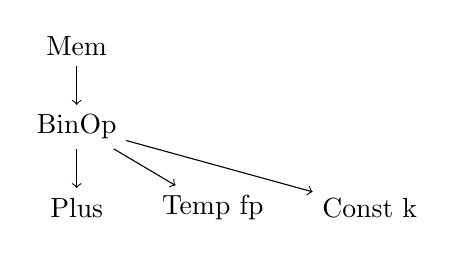
\begin{tikzpicture}
    \node(mem) {Mem};
    \node(binop) [below = 0.5cm of mem]{BinOp};
    \node(plus) [below = 0.5cm of binop] {Plus};
    \node(temp) [right = 0.5cm of plus] {Temp fp};
    \node(const) [right = 0.5cm of temp] {Const k};
    
    \draw [->] (mem) -- node[left, pos=0.2] {} (binop) ;
    \draw [->] (binop) -- node[left, pos=0.2] {} (plus) ;
    \draw [->] (binop) -- node[left, pos=0.2] {} (temp) ;
    \draw [->] (binop) -- node[left, pos=0.2] {} (const) ;
  \end{tikzpicture}

  Use Semant module to provide access of variable, level of function where variable is used to translate module function, and get back a \verb%TrExp%

\begin{verbatim}
TrSimpleVar(TrAccess, TrLevel) -> TrExp
\end{verbatim}

  where:\\
  \verb%TrAccess% contains level of variable declaration\\
  \verb%TrLevel% is the level of variable use

  Turning \verb%FrAccess% (formals and local variables allocated in frame/register) into IR expression:
\begin{verbatim}
FrExp(FrAccess, TrExp) -> TrExp
\end{verbatim}
  where:\\
  \verb%TrExp% is the frame pointer where \verb%FrAccess% lives, calculated via static links (variable may be in different static nesting level); ignored if variable is in register.
  \verb%TrExp% is the generated IR with pointer and offset calculations

  Calculating \verb%TrExp% using static links for SimpleVar:

  \verb%tr_exp = Mem(+(Const% $k_n$, \verb%Mem(+(Const% $k_{n-1}$\verb%, ..%\\
  \verb%  Mem(+(Const% $k_1$, \verb%Temp fp))..)%

  where:\\
  $k_1,..,k_n$ are static link offsets in nested functions\\
  \verb%fp% is the current frame pointer of where the variable is used

  let $l_f$ be the level of function $f$ where variable is used\\
  let $l_g$ be the level of function $g$ where variable is declared\\
  then $l_f - l_g$ static link offsets are followed to calculate variable location where it is originally declared

  \subsection{Large Variable}
  Eg: arrays and records

  Implementation variations:
  \begin{itemize}
  \item pointers: assignment means pointer assignment
  \item content as value: assignment means copying entire value
  \end{itemize}

  \subsection{Structured l-value}
  large values that don't fit in 1 word\\
  data structure may need additional info for size\\
  eg: \verb%Mem% operator needs size parameter:\\
  \verb%TrMem(TrExp, size) -> TrExp%\\
  \verb%Mem(+(Temp fp, Const k), S)%

  \subsection{Subscript/Field Selection}
  Compute offset from  a base to get a component of interest

  \subsection{Array subscript expression}
  \begin{itemize}
  \item l-value for base and smaller subranges
  \item l-value coerced to r-value via \verb%Mem% operator in cases of:\\
    1) pass by value, 2) assignment to another array variable
  \end{itemize}

  \subsection{Language without structured l-value}
  Pointers are passed instead where base address of l-value object is the value stored in a pointer variable $\implies$ an additional \verb%Mem% operator is required to ``deref'' the pointer.

  accessing element of width w at index i of an array with base address stored in variable e:\\
  \verb%Mem(Plus((Mem e), BinOp(Mul, i, Const w)))%

  analogous to \verb%*(*e + i*w))% in C code

  l-value is technically an address without \verb%Mem% operator.

  \subsection{Error detection for out of bounds component access}
  \begin{itemize}
  \item compile time checks desirable
  \item nullptr checks before deref
  \end{itemize}

  \subsection{Convert if else to conditional jump}
  convert \verb%if a then b else c% to conditional jump:
  \begin{itemize}
  \item use of temporary and true/false labels
  \item move instruction to temporary in branches
  \item use of \verb%un_cx(a), un_ex(b), un_ex(c)%
  \item 1 final join label for branches
  \item eg: nested conditionals:\\
    \verb%Seq(cx(s_1,z,f), Seq(z, cx(s_2,t,f)))%
  \end{itemize}

  \subsection{String comparison}
  use of external runtime routine via \verb%Call% node

  \subsection{Long lived objects allocated on the heap}
  \begin{enumerate}
  \item call a runtime function to allocate space and return pointer to a temporary \verb%r%
  \item do a series of \verb%Move%s using returned pointer and offsets to initialize large values
  \item reading the expression is \verb%Temp(r)%
  \end{enumerate}

  \subsection{Calling external runtime function}
  \verb%Call(Name(NameLabel("init_array")),%\\
  \verb%  TrExpList(a, TrExpList(b, null)))%\\
  $\iff$ \verb%init_array(a,b);%

  Possibly wrap in a helper in Frame module:\\
  \verb%Fr::external_call(f: String, args: TrExpList) -> TrExp%

  \subsection{Function call}
  \verb%Call(l: NameLabel, args: [sl, e_1, e_2, ..])%\\
  where:\\
  \verb%l%: label of function to call\\
  \verb%sl%: static link (address of frame of enclosing function)\\
  \verb%e_1, e_2, ...%: other normal arguments

  \subsection{Declarations}
  \verb%trans_dec(..)% also side-effects the frame data structure:
  \begin{itemize}
  \item per variable declaration: additional space will be reserved in current frame
  \item per function declaration: new ``fragment'' of code will be kept for function body
  \item variable initialization / definition:
    \begin{itemize}
    \item translates to an expression, put before the ody of \verb%let% expression
    \item return \verb%TrExp% containing assignment expressions that accomplish initializations of variables
    \end{itemize}
  \item function definition: translation to a segment of assembly language with:
    \begin{itemize}
    \item prologue: setup instructions for function call
    \item body: containing body expression translation
    \item epilogue: teardown instructions for function call
    \end{itemize}
  \end{itemize}

  \subsubsection{prologue}
  \begin{itemize}
  \item pseudo instruction for an assembly language
  \item label definition for function name
  \item instructions to adjust stack pointer in allocating new frame
  \item instructions to save escaping arguments into frame (including staic link)
  \item instructions to move non-escaping arguments into fresh temporary registers
  \item store instructions to save callee-save registers (eg: return address register)
  \end{itemize}

  \subsubsection{Epilogue}
  \begin{itemize}
  \item instruction to move return value to register reserved for the purpose
  \item load instructions to restore callee-save registers
  \item instruction to reset stack pointer (frame deallocation)
  \item return instructions (jump to return address)
  \item announce end of function to assembler
  \end{itemize}

  Many of these info (eg: exact frame size) are unknown until later, so these instructions need to be generated late in the compilation process

  \subsection{Procedure Fragments}
  Using:
  \begin{itemize}
  \item already translated function body expression, and
  \item function definition with a static nesting level
  \end{itemize}
    
  Translate phase should:
  \begin{itemize}
  \item produce a descriptor for function containing necessary information:
    \begin{itemize}
    \item frame descriptor with machine specific info. about local variables and parameters
    \item result returned from a helper function that does restore of registers and moving incoming formal parameters
    \end{itemize}
  \item define an interface within Translate module via a frag datatype (this gets accumlated into a list during translation of procedures)
  \end{itemize}
  
  \vfill\null
  \columnbreak

  \section{Basic Blocks, Traces}
  Goal: transform structure of tree nodes (IR) so that resulting trees are in a canonical form that can be further linearized and reordered without unsoundness

  Strategy:
  \begin{itemize}
  \item pull ESEQs out of list of expressions/statements and lift them to the top of the tree; these get transformed into SEQs; linearize them into sequential instructions
  \item restrict CALLs to occur only under specific types of node: \verb%EXP(..), MOVE(TEMP(t, ..))%
    \item parent of a \verb%SEQ% node can only be a \verb%SEQ% node
  \end{itemize}

  \subsection{Lifting ESEQ out of expressions}
  $\text{ESEQ(s, e)} = e_{\text{original}}$\\
  where by definition of ESEQ, $s$ is executed before $e$

  use equivalence identities for transformations of nodes (TODO)

  use of commutativity simplifies transformations but hard to know if it's applicable to an expression in general

  \subsection{Trace construction}
  Goal: generate a set of traces that cover the entire program\\

  Sample algo:
  \begin{itemize}
  \item grow a trace from a selected basic block: when encountering a cjump/jump (at the end of the block), continue trace by selecting a possible path and adding the selected block to the current trace
  \item delete jump instruction afterwards
  \item trace stops growing when successors to current frontier block are already covered by existing trace(s)
  \end{itemize}

  \subsection{General Procedure}
  \begin{enumerate}
  \item linearize: list of statements (T\_stm) $\rightarrow$ canonical trees (T\_stmList): apply rewrite rules: ESEQs removed, CALLs restricted to be under nodes of certain types
  \item group into basic blocks: canonical trees $\rightarrow$ basic blocks (these now can be reordered arbitrarily)
  \item trace schedule: basic blocks $\rightarrow$ T\_stmList: a set of traces covering entire program
  \end{enumerate}

  \subsection{Rewrite Rules}

  \subsubsection{Reorder}
  \verb%reorder([expr]) -> stm%

  Goal
  \begin{itemize}
  \item pull ESEQs out of given list of expressions
  \item combine statement parts of ESEQs together into 1 sequence and return as statement
  \item rewire nodes with ESEQ child node to point to new expression as child instead
  \end{itemize}

  Delegate to \verb%do_exp(..)%, \verb%do_stm(..)%
      
  \subsubsection{Expr Rewrite}
  \verb%do_exp(expr) -> ESEQ(stm',expr')%

  Goal: pull out statements out of given expression and return ESEQ(s,e) where it is equivalent to original expression

  Recursively call reorder when necessary depending on expression type.

  \subsubsection{Statement Rewrite}
  \verb%do_stm(stm) -> stm%

  Goal: pull out ESEQs out of a statement and reorder to return ordered statement

  Recursively call reorder when necessary to apply rewrite rule on sub-expressions of the statement.

  \subsubsection{Linearize}
  \verb%linearize(stm) -> [stm]%

  Goal
  \begin{itemize}
  \item flatten parts of the tree previously processed by rewrite rules where all SEQ nodes are at the top
  \item return a list of statements where SEQs are eliminated
  \end{itemize}

  Apply \verb%linearize(do_stm(..))% on body of target function to get back linearized statements.

  Pass the resulting list of statements to constructor of basic blocks.

  \subsection{Basic Block Properties}

  Construct basic block(s) from list of linearized statements with the following invariants by adding labels, modifying jumps, starting new blocks as necessary.

  \begin{itemize}
  \item a label is at the start of the block
  \item a cjump/jump is at the end of the block
  \item no other jumps exist in any other part of the block
  \end{itemize}

  \subsection{Trace Schedule}
  
  Goal
  \begin{itemize}
  \item reduce amount of jump overhead by combining basic blocks
  \item placement of false label to fall through for conditional jump
  \end{itemize}

  Strategies
  \begin{itemize}
    \item Reorder blocks so unconditional jumps are followed immediately by destination blocks and these blocks can be added to a same trace, so that jumps can be eliminated later.
    \item Reorder blocks so condition jumps are followed immediately by blocks with false label, invert conditional logic if necessary. This allows better mapping to branching instruction on most hardware where false label jumps can be eliminated later.
  \end{itemize}

  Sample iterative algo.: grow current trace with a work list of basic blocks and looking at uncovered successor blocks of current block.
    
  \vfill\null
  \columnbreak

  \section{Instruction Selection}

  Goal: cover the IR tree with a minimal set of instruction patterns that are non-overlapping, typically using an idealized cost model for selection
  
  \subsection{Sample Tiling Selection Algos}
  \subsubsection{Maximal Munch}
  \begin{itemize}
  \item Greedy, locally optimal
  \item Top down growth of tiles starting from the root
  \item sample strategy: select a tile of the largest size that is feasible and rooted at the current node (looking at node type)
  \item if there exists a tile for every node type of the tree, then algo will not get stuck
  \item process sub-expressions and statements recursively: \verb%munch_exp(..)%, \verb%munch_stm(..)%
  \end{itemize}

  \subsubsection{Dynamic Programming}

  \begin{itemize}
  \item Globally optimum
  \item bottom up traversal and compute minimal accumulated cost at current node: cost of a feasible tile rooted at current node plus subtree costs of its child tiles
  \item 2nd pass to emit instructions based on selected tiles in post order (emit instr for rooted nodes of child tiles, emit instr for the tile rooted at current node)
  \end{itemize}

  \subsection{Register Allocation Pass}
  schedule register allocation pass after instruction selection means instruction selection needs to work without exact registers $\implies$ use an abstraction for instructions without register (Abstract Assembly Language Instructions), which is independent of target machine assembly language.

  \subsection{Abstract Assembly Language Instructions}
\begin{verbatim}
  enum AsInstr {
    Oper(
      asm: string,
      dst: [NameTemp],
      src: [NameTemp],
      jumps: [NameLabel]),
    Label(
      asm: string,
      label: NameLabel),
    Move(
      asm: string,
      dst: [NameTemp],
      src: [NameTemp]),
  }
\end{verbatim}

  \begin{itemize}
    \item \verb%[NameTemp]%: list of registers assigned by register allocator
    \item Oprations that fall through $\implies$ \verb%jump% is empty
    \item \verb%Label%: point in program that \verb%jump%s can go
    \item \verb%asm% instruction does not know about register assignments; use generic enumerations \verb%s<n>, d<n>, j<n>%, eg: \verb% LOAD d0 <- M[s0 + 0]%
    \item \verb%asm% instruction may have registers that are both used for src and dst
    \item After choosing temporaries by instruction selector: \verb% LOAD d0 <- M[s0 + 0]; dst:[t909], src: [t92]%
    \item After register allocation, sample asm:\\
      \verb%LOAD r2 <- M[r12+0]%
  \end{itemize}
    
  Use of \verb%AsInstr% during IR tiling selection phase:
  \begin{itemize}
  \item \verb%munch_exp(..), munch_stm(..)% to emit instructions (accumulate instructions into a sequence)
  \item \verb%munch_exp(..)% returns temporary of the expression result
  \item sample \verb%munch_exp%:
\begin{verbatim}
  fn munch_exp(e) {
    match e {
      MEM(BINOP(PLUS, e1, CONST(i))) => {
        let r: NameTemp = NameTemp::new();
        emit(AsOper(
          asm=format("LOAD d0 <- M[s0 + {}]", i),
          dest=[r],
          src=munch_exp(e1):[],
          jumps=[]));
        return r;
      },
      CONST(i) => {
        let r: NameTemp = NameTemp::new();
        emit(AsOper(
          asm=format("ADD d0 <- r0 + {}", i),
          dest=[r],
          src=[],
          jumps=[]));
        return r;
      },
      ..
    }
  } 
\end{verbatim}
    note special \verb%r0% register for zero value
  \item sample \verb%munch_stm%:
\begin{verbatim}
  fn munch_stm(s) {
    match s {
      MOVE(TEMP(i), e2) => {
        emit(AsMove(
          asm="ADD d0 <- s0 + r0",
          dest=[i],
          src=munch_exp(e2):[]));
      },
      MOVE(MEM(CONST(i)), e2) => {
        emit(AsOper(
          asm=format("STORE M[r0+{}] <- s0",i),
          dest=[],
          src=munch_exp(e2):[],
          jumps=[]));
      },
      ..
    }
  } 
\end{verbatim}
  \end{itemize}
  
  \subsubsection{NameMap utility}
  new() $\rightarrow$ NameMap\\
  query(NameMap, NameTemp) $\rightarrow$ string\\
  update(NameMap, NameTemp, string)\\
  layer(over: NameMap, under: NameMap) $\rightarrow$ NameMap

  Use cases for NameMap:\\
  register allocator: temporary $\rightarrow$ register name\\
  frame module: preallocated register $\rightarrow$ register name\\
  debugging: temporary $\rightarrow$ stringified name

  \subsubsection{Procedure calls}
  \begin{itemize}
  \item
\begin{verbatim}
  EXP(CALL(e, args)) => {
    let r: NameTemp = munch_exp(e);
    let l: [NameTemp] = munch_args(args);
    emit(AsOper(
      asm="CALL s0",
      dest=calldefs, //mutated registers from call
      src=r:l,
      jumps=[]));
  }
\end{verbatim}
    
  \item  Use of utility function \verb%munch_args(..) -> [NameTemp]% to generate code to move all arguments to correct positions in registers and/or memory. Returned temporaries pass in as sources to the instruction (may not be explicitly written in assembly language) in order for liveness analysis to work correctly.
  \item Call may side-effect registers (caller-save, return-address, return-value) $\implies$ list involved registers as destinations in order for later analysis to know they get affected.
  \end{itemize}

  entry point, passing rewritten/reordered statements (of a function body) that are processed by earlier phases:
\begin{verbatim}
  fn codegen(stm_list: [T_stm]) -> [AsInstr] {
    for s in stm_list {
      munch_stm(s);
    }
    INSTR_LIST
  }
  fn emit(instr: AsInstr) -> () { 
    INSTR_LIST = INSTR_LIST ++ (instr: [])
  }
\end{verbatim}  

  \vfill\null
  \columnbreak

  \section{Liveness Analysis}

  \subsection{Definitions}

  $succ[n]=\{x:\text{n has an arrow to x}\}$ (nodes connected by outgoing edges)\\
  $pred[n]=\{x:\text{x has an arrow to n}\}$ (nodes connected by incoming edges)

  assignment to variable/temporary defines that variable:\\
  $def[n]=\{v:\text{node n defines variable v}\}$

  variable on right hand side of assignment uses the variable:\\
  $use[n]=\{v: \text{node n uses variable v}\}$
  
  $def(var)=\{n: \text{node n defines variable var}\}$

  $use(var)=\{n: \text{node n uses variable var}\}$

  liveness: variable is live on an edge if there exists a directed path from the edge to use of that variable that does not go through a def

  live-in ($in[n]$): variable is live on $\geq 1$ in-edge(s) of that node

  live-out ($out[n]$): variable is live on $\geq1$ out-edge(s) of that node

  \subsection{Dataflow Equations for Solving Liveness Range}
  
  $in[n]=use[n] \cup (out[n] \setminus def[n])$\\
  $out[n]=\cup_{s\in succ[n]} in[s]$

  Solve via:
  \begin{itemize}
  \item fixed point iteration, or
  \item per variable search backwards (starting at use and ending on a definition of the variable)
  \end{itemize}
  
  Liveness flows backwards, so perform iteration of dataflow equations in reverse order of control flow graph).

  Merging of nodes to basic blocks $\implies$ allows faster perfomance due to reduced number of graph elements.

  \subsection{Complexity}
  Worst case: outer loop of fixed point iteration $O(N^2)$ due to bounding of in-set/out-set to $N$ elements.\\
  Set operation between nodes: $O(N^2)$. Then overall worst case is $O(N^4)$\\
  Reordering of nodes $\implies$ outer loop usually needs 2-3 iterations.\\
  Live-sets sparse $\implies O(N)$ to $O(N^2)$ in most cases.

  \subsection{Solutions to Dataflow Equations}
  may be approximations:\\
  live variables present in approximation\\
  presence of variable in approximation that may not need to be live

  \subsection{Static vs. Dynamic Liveness}
  Special case algo. can improve liveness analysis in some cases

  Dynamic liveness:\\
  variable $a$ is dynamically live at node $n$ if some execution of the program goes from $n$ to use of $a$ without going through a definition of $a$.

  Static liveness:\\
  variable $a$ is statically live at node $n$ if there exists a path of control flow edge from $n$ to some use of $a$ that does not go through a definition of $a$.

  dynamically live $\implies$ statically live

  In general, optimize using static liveness for approximation

  \subsection{Liveness for Register Allocation}
  overlapping live ranges of temporaries $\implies$ use separate register at that point of execution

  interference graph: expressing non-overlapping live range constraints between pairs of variables using edges

  \subsection{Move Instruction Optimization}
  
  no need to create an interference edge for \verb%t <- s%
  
  however if a later non-\verb%Move% definition of \verb%t% happens, interference still needs to be accounted at that point

  algo:
  \begin{itemize}
  \item definition of \verb%a% at non-move instruction $\implies$: add interference edge between sources and destination (\verb%a%) variables.\\
    interference edges: $\{(s, a)\}, \forall s \in \text{sources}$
  \item definition of \verb%a% at move instruction \verb%a <- c%: if variable \verb%b% is live-out and \verb%b% $\neq$ \verb%c% $\implies$ add interference edge $(a, b)$; eg: \verb%b% will be used later
  \end{itemize}
  
  \subsection{Control Flow Graph Module}
  Construct a control flow graph. Use this later to perform liveness analysis of variables and produce an interference graph.

  Use a module, FlowGraph, to manage nodes:
  \begin{itemize}
  \item node represents instruction/ basic block
  \item instruction \verb%m% can be followed by instruction \verb%n% $\implies$ edge $(m, n)$ exists in graph
  \item internal data of FlowGraph hidden from outside behind an interface
  \item let nodes represent abstract instructions; take in a list of instructions and return flow graph where info of node is abstract assembly instruction
  \item jump fields of instruction used in creating control flow edges
  \item source and destination fields of instructions used to obtain use and def information
  \end{itemize}

  Info associated with each node:\\
  \verb%FlowGraph::def(n) -> {t: temporary t defined at node n}%\\
  \verb%FlowGraph::use(n) -> {t: temporary t used at node n}%\\
  \verb%FlowGraph::isMoveInstruction(n) -> bool%\\
  
  Separate association of node to extra info possible by an external mapping function.  

  \subsection{Liveness Module}
  Takes in a flow graph and produces:
  \begin{itemize}
  \item interference graph
  \item list of node(variable)-pairs representing Move instructions that may be elided in later phases of compilation
  \end{itemize}

  Interference graph node \verb%n%:\\
  \verb%Live::temp(n) = temporary variable represented by node n% ($n \mapsto NameTemp$)

  Maintain data structure for remembering what is live at exit of each flow graph node (live-out)

  Calculation of \verb%live_map% (set of live temporaries at current location) used to construct interference graph:\\
  ($\forall$ flow node $n$)($\forall d \in def[n]$)($\forall i$) add interference $(d, t_i)$\\
  where:\\
  $\{t_1, t_2, ..\} \equiv$ temporaries in \verb%live_map%\\
  $def[n]\equiv$ newly defined temporaries at node $n$

  \subsubsection{Zero Length Live Range}
  Definition may include side effects (eg: write to regsiter, even if variable is not used after)
  
  May interfere with any overlapping live ranges.

  Therefore 0-length live range needs to be taken into account.
  
  
  \vfill\null
  \columnbreak

  \section{Register Allocation}

  Goal: colour nodes of interference graph:
  \begin{itemize}
  \item no 2 adjacent ndoes are coloured the same
  \item minimize number of colours used
  \item a colour corresponds to a specific register
  \end{itemize}

  General phases:\\
  1. define an order of nodes\\
  2. colour nodes in defined order while preserving colour invariant

  \subsection{Common Algorithm}
  Phases: build, simplify, coalesce, freeze, potential spill, select

  \begin{tikzpicture}
    \node(build) {build};
    \node(simplify) [below = 0.5cm of mem]{simplify};
    \node(coalesce) [below = 0.5cm of simplify] {coalesce};
    \node(freeze) [below = 0.5cm of coalesce] {freeze};
    \node(spill) [below = 0.5cm of freeze] {spill};
    \node(select) [below = 0.5cm of spill] {select};
    \node(end) [below = 0.5cm of select] {end};
    
    \draw [->] (build) -- node[left, pos=0.2] {} (simplify) ;
    \draw [->] (simplify) -- node[left, pos=0.2] {} (coalesce) ;
    \draw [->] (coalesce) -- node[left, pos=0.2] {} (freeze) ;
    \draw [->] (freeze) -- node[left, pos=0.2] {} (spill) ;
    \draw [->] (spill) -- node[left, pos=0.2] {} (select) ;
    \draw [->] (select) -- node[left, pos=0.2] {} (end) ;

    \path [line] (coalesce) --++ (1cm,0cm) |- (simplify);
    \path [line] (freeze) --++ (1cm,0cm) |- (simplify);
    \path [line] (spill) --++ (1cm,0cm) |- (simplify);
    \path [line] (select) --++ (2cm,0cm) |- (build);
  \end{tikzpicture}

  \subsubsection{Build}
  Construct interference graph for register resident variables (create edges for temporaries that have overlapping live ranges). Mark node as move / non-move.

  \subsubsection{Simplify}
  Put nodes in some stack order.

  For non-move nodes, if there exists a node from graph that has $<k$ (where $k$ is the number of available registers) degree $\implies$ add it to stack (and remove from graph), otherwise go to potential spill phase.
  
  \subsubsection{Coalesce}
  Tentatively merge nodes (assigned same colour) based on some safe algoithm (eg: Briggs / George), and go to simplify step. Repeat until all nodes remain have $\geq k$ degree or are only move-related nodes.

  Potentially coalesce move-related nodes and thus delete move instructions. If no edge exists between src and dest. of move instruction $\implies$ edges are coalesced when src and dest. nodes merge.

  Coalescing makes nodes with more edges in general, safe strategies used (if original graph is colourable, and if applying safe strategy for coalescing is successful then the result is also colourable).

  Briggs:\\
  Nodes $a$ and $b$ merged has $<k$ neighbours of significant degree ($\geq k$ edges) $\implies$ can be merged

  George:\\
  all neighbours of $a$ either interferes with $b$ or $<k$ degree $\implies$ can be merged

  interleaving of simplify and coalescing phases is effective at removing redundant move instructions while not introducing spills.

  \subsubsection{Freeze}
  At this stage, all nodes are $\geq k$ degree or move-related.
  
  If possible, select move node of low degree and mark it as non-move (give up coalescing), and go to simplify step.

  \subsubsection{Potential Spill}
  If there exists no $<k$ degree node, select a node (eg: of highest degree) to be potentially represented in memory instead of register (edges in graph removed) and push onto the stack, and go to simplify step. Repeat until no spill occurs (remaining nodes have $< k$ degree) and all nodes have been simplified and added to the stack. Optimistic colouring heuristic: select node with high degree to remove, continue process and hope that node will eventually be colourable after more removal.

  \subsubsection{Select}
  Pop all nodes from stack and try assigning colours.\\
  Either assignment is successful, or if not assignable: rebuild the graph by inserting instructions to relocate variable to memory (actual spill occurs), discard coalesces found in this round, and go to build step.

  If all assignments are succesful, then the algorithm ends successfully.

  \subsection{Coalescing of Spilled Nodes}

  \begin{itemize}
  \item spill pairs are ususally never live simultaneously since number of memory locations aren't practically bounded
  \item use liveness information to construct interference graph for spilled nodes
  \item if there is a pair of non-interfering spilled nodes connected by move instruction, then coalesce them
  \item use simplify and select to colour the graph; no spilling occurs here\\
    simplify: picks lowest degree node\\
    select: picks 1st available  colour (no limit on number of colours here due to plentiful memory addresses)
  \item colours correspond to activation record locations of spilled variables
  \item performed before generating spill instructions and interference graph of register-resident temporary (register allocation for remaining nodes) to avoid fetch-store sequences for coalesced moves of spilled nodes.
  \end{itemize}

  
  \subsection{Precoloured Nodes}

  These don't simplify (no freedom of assigning an arbitrary colour) and spill (can't spill to memory since these are specific to register)

  Generated for certain calling conventions where particular temporaries are permanently bound to certain registers (eg: frame pointer, standard argument 1 register)

  Ordinary temporaries may be assigned same colour as precoloured register as long as they don't interfere.
  
  Desirable: Keep live ranges of precoloured nodes short. Use move instructions to assign to fresh temporaries (these can be spilled) before moving it back to precoloured register when needed.\\
  Eg: callee-save registers\\
  May be coalesced and move eliminated back to original if there isn't register pressure.

  \subsection{Optimization}
  \begin{itemize}
  \item variable not live across procedure call $\implies$ allocate to caller-save register to save extra instructions
  \item variable live across procedure call $\implies$ keep in callee-save register
  \item specialized allocation algo. on expression trees is efficient
  \end{itemize}

  \subsection{Kempe Graph Colouring}

  heuristic for phase 1 of graph colouring (defining an order of nodes)
  
  Solve subproblem recursively until base case:
  \begin{itemize}
  \item there are $\leq k$ nodes remaining in graph $\implies$ graph is colourable, or
  \item remove a node with $< k$ degree and push onto stack for later colour assignment
  \end{itemize}
  
  \subsection{Algo}
\begin{verbatim}
fn reg_alloc(){
  liveness_analysis();
  build();
  make_worklists();
  while !all_worklists_empty() {
    if !simplify_worklist.empty() { simplify(); }
    if !move_worklist.empty() { coalesce(); }
    if !freeze_worklist.empty() { freeze(); }
    if !spill_worklist.empty() { select_spill(); }
  }
  assign_colours();
  if !spilled_nodes.empty() {
    rewrite_program(spilled_nodes);
    reg_alloc();
  }
}
\end{verbatim}
  
  \vfill\null
  \columnbreak

  \section{GC}

  goal: minimize number of reachable record that are not live

  \subsection{Mark and Sweep}

  traverse directed graph to mark all reachable nodes

  unmarked nodes at end of sweep are garbage and can be reclaimed (via freelist)

  reset marks of all nodes for next sweep

  use of freed memory to use as stack vs. explicit stack (threading pointers in free nodes)

  sweeping phase: put unmarked records into freelist (can use different freelists for different sized records)

  issues: external vs. internal fragmentation

  \subsection{Reference Counts}

  record contains additional info on the nummber of pointers pointing to the record

  increment number when pointer is stored to somewhere

  decrement when pointer is removed from somewhere

  when number is 0 $\implies$ put record into freelist; recursively decrement internal pointers in record during allocation (removal from freelist) for shother GC pauses

  issues: cycles cannot be reclaimed (count never reaches 0) even if not reachable from program

  incrementing ref counts is costly (due to instructions for putting things into freelists and possibly decrementing previous pointer records)

  may be optimized by aggregating count updates via dataflow analysis

  \subsection{Copying Collection}

  division of space into to-space and from-space

  compacting copying

  easy to allocate

  pointer forwarding: operations to copy a pointer in from-space to to-space correctly

\begin{verbatim}
fn forward(p) {
  if p.is_in_from_space(){
    if p.f1.is_in_to_space(){
      return p.f1
    }
    for i in p.fields() {
      next.field(i) = p.field(i);
    }
    p.f1 = next;
    next = next + sizeof(p);
    return p.f1
  }
  p // already in to-space
}
\end{verbatim}
  
  BFS copying GC (Cheney's algo.):
  \begin{itemize}
  \item scan and next cursors
  \item 1st forwarding of root objects
  \end{itemize}

\begin{verbatim}
scan = next = start_of_to_space
for r in roots {
  r = forward(r);
}
while scan < next {
  record = get_record_at(scan);
  for i of record.fields(){
    scan.field(i) = forward(scan.field(i));
  }
  scan = scan + sizeof(record);
}
\end{verbatim}
  
  start of to-space $\leq$ scan $\leq$ next

  area between scan and next may contain pointers not yet forwarded (still points to from-space)

  issues: locality of reference

  variant of algo: depth first copying

  cost: $O(\text{number of nodes marked})$

  ammortized cost (per word allocated): $\frac{c R}{\frac{H}{2} - R}$


  \subsection{Generational Collection}

  effective when old objects rarely update to point to new objects

  objects promoted to older generation area after surviving a few collections

  collect by: mark and sweep, or copying collection

  in addition of root nodes, we keep a set of objects from older generations (remembered set) that have updated to point to objects in newer generations; these are scanned to update the pointers when objects in newer generations are copy collected to new to-space
  \begin{itemize}
  \item insert extra instructions when updating pointer field: put object into a set of updated objects that gets scanned for pointers back to $G_0$
  \item runtime GC gets this set to run its algo.
  \end{itemize}
  
  from-space $\equiv G_0$ arena hemisphere

  roots $\equiv$ program variables + remembered set

  to-space $\equiv G_0$ arena new hemisphere

  pointers to older generations not changed

  marking algo.: not mark objects in older generations

  copying algo.: copies these verbatim without forwarding

  after several collection of $G_0$, run collection for $G_0$ and $G_1$:
  \begin{itemize}
  \item remembered set for roots contained in $G_1, G_2, ..., G_k$
  \item collect $G_0$ nad $G_1$ together
  \end{itemize}

  \subsection{Incremental Collection}
  
  interleave collection work in order to avoid long interruptions

  types:
  \begin{itemize}
  \item incremental: collector operates only when mutator (program changing graph oof reachable data) requests it
  \item concurrent: collector can operate between any instructions executed by mutator
  \end{itemize}

  classes of records:
  \begin{itemize}
  \item white: objects not yet visited by DFS/BFS
  \item grey: objects that have been marked/copied, but childrens have not been examined
  \item black: objects that have themselves and their children marked
  \end{itemize}

  generalization of mark-and-sweep and cpoying collection algo: tricolour marking algo.

\begin{verbatim}
while let Some(p) = grey_objects() {
  for i in p.fields(){
    if p.field(i).is_white() {
      p.field(i).colour = grey
    }
  }
  p.colour = black
}
\end{verbatim}

  invariants that a mutator respects:
  \begin{itemize}
  \item no black object points to a while object
  \item every grey object is on collector's stack/queue/data structure (grey-set)
  \end{itemize}

  incremental algo variants:
  \begin{itemize}
  \item Dijkstra, Lamport, et. al.
  \item Steele
  \item Boehm, Demers, Shenker
  \item Baker
  \item Appel, Ellis, Li
  \end{itemize}

  general types of implementation:
  \begin{itemize}
  \item write barrier algo: write/store by mutator checked to make sure invariant is maintained
  \item read barrier algo: read/fetch instructions checked for invariant
  \end{itemize}
  these must synchronize with collector:
  \begin{itemize}
  \item using software implementations of barrier: explicit synchronization instructions (may be expensive)
  \item use of virtual memory H/W (sync. implicit in a page fault (mutator faults on a page $\implies$ O/S ensures no other process has access to that page before processing the fault
  \end{itemize}

  \subsubsection{Baker's Algorithm}
  example of an incremental copying collection algo.

  TODO
  
  \subsection{Interface to the Compiler}
  live analysis: derived pointer implicitly keeps its base pointer live so the GC algo. does not get confused by elimination of pointers in live analysis

  use of inline expansion and merge ops from multiple allocations to save instruction related to allocation with GC

  \subsubsection{GC Layout of Objects}
  OO language contains class descriptors (compile time generation) in every object for dynamic lookup $\implies$ no additional per-object cost if these are also used for GC

  Compiler needs to signal to GC collector every pointer containing temporary and local variable (in register or activation record)

  set of live temporaries different at every point in the program $\implies$ more efficient to describe pointer map at points where new GC cycle can begin:
  \begin{itemize}
  \item calls to alloc function
  \item each function call (since they can laso call alloc)
  \end{itemize}
  example impl.: map function return address to live pointer set: for all pointer live immediately after call, map tells their register/frame location

  root finding:
  \begin{itemize}
  \item collector starts at top of the stack and scans downward frame by frame
  \item in each frame, collector marks/forwards (if using copying collection) pointers in that frame (these pointers are obtained from address map to pointer entries)
  \item callee-save registers with special handling:\\
    function must describe which of its callee-save registers contain pointers at call to another function via additional info in pointer map so that the called function knows which callee-saved registers contain pointers
  \end{itemize}
  
  \vfill\null
  \columnbreak

  \section{Extensions with OOP}

  Static methods: find method using ancestor chain.

  Dynamic method: a list of method instances in class descriptor ( from ancestor classes in the case of single inheritence tree).

  Method for field initialization for class objects.

  Method instance lookup for multiple inheritance can use static analysis for packing:
  \begin{itemize}
  \item Compile time hashing of fields/methods to offsets/code addresses.
  \item Graph colouring: add edge between fields that exist in its class and ancestor classes (these are the ones that cannot coexist). A colour corresponds to a slot. May end up with vacant slots due to colouring constraints.
  \end{itemize}

  \subsection{Compaction}
  Pack fields and methods in class object instances; map uncompacted slots to compacted offsets in a separate descriptor which is shared between many class objects.

  Field lookup: in class object instance, fetch descriptor pointer. Fetch field offset from descriptor, perform store/fetch on data at offset wrt. object.
  Further perform static analysis to elide extraneous operations (eg: common expressions).

  \subsection{Class Membership Test}
  Use class descriptor info to compare against class type tags.
  
  Use linked list of base classes.

  \subsection{Type Coercion}
  \begin{itemize}
  \item sub to base class coercion safe at compile time
  \item base to sub class coercion requires runtime type check and exception support
  \item static/runtime casts/tests usually needs language support
  \item conditional test allows compiler to apply type narrowing/coercion and type propagation optimization on relevant code paths
  \end{itemize}

  \subsection{Private Members}
  Type check phase enforces it.

  Implemenation can simply use an indicator information for each member in symbol table. Uses of members require checking the indicator.

  \subsection{Converting dynamic calls to methods to static method calls}
  Less execution pipeline stalls due to runtime indirections.
  
  Determination:
  \begin{itemize}
  \item When method call is always with the same method instance, then replace dynamic call with static call
  \item use subclass info, if no overrides for method call exist then use static call at call site
  \item static dataflow analysis: type propagation from declaration/assignment to call sites may constrain the possible method instances at call sites
  \end{itemize}
  
  \vfill\null
  \columnbreak

  \section{Extensions with FP}

  Flavours of FP:
  \begin{itemize}
  \item impure and higher order (function as argument / return value of function)
  \item strict and pure
  \item non-strict and pure
  \end{itemize}

  Techniques for saving/accessing non-local environment:
  \begin{itemize}
  \item lambda lifting
  \item closure with code pointer and static link\\
    Without nesting of functions: machine code address of function (and representation of function in some variable)\\
    With nesting of functions: machine code pointer and access to non-local variable used by function (such as through static link)
  \end{itemize}

  \subsection{An impl of code pointer and non-local variable access via static link}
  
  Heap allocation for either:
  \begin{itemize}
  \item entire activation record of function
  \item only variables that escape (used by inner functions); let stack frame's variable point to heap allocated escape variable record
  \end{itemize}

  Escape variable record:
  \begin{itemize}
  \item heap allocated record containing local variables that is needed by inner functions
  \item static link to environment (escape variable record) provided by enclosing function
  \end{itemize}
  
  Cleanup / recycle via garbage collector

  Static Link:
  \begin{itemize}
  \item access free/non-local variables (eg: the environment)
  \item passed in as an argument to function
  \item stored in a record on the heap
  \end{itemize}

  Pointer to escape variable record:
  \begin{itemize}
  \item accessible in stack frame
  \item not escape and therefore can be spilled
  \end{itemize}

  When allocating formal parameters and local variables:
  \begin{itemize}
  \item escape variables allocated to a record on heap
  \item calculation of offsets uses escape variables record when walking the static link chain
  \end{itemize}

  \subsection{Pure FP Language}
  
  Immutability of variables allows equational reasoning:
  \begin{itemize}
  \item variable assignment only happens once
  \item side effects disallowed
  \end{itemize}

  COW for producing new values
  
  GC recycles unreachable variables

  Optimizations:
  \begin{itemize}
  \item control flow graph: more complex due to function variables that are not statically defined
  \item equational reasoning (with immutable variables): can replace variable values with constraints once value propagation has been performed
  \item inline expansion
    \begin{itemize}
    \item renaming of parameter/variable to avoid name clases
    \item replacement of formal parameters and their occurences in function body by new and unique variables using let declarations
    \item after inlining, unreferenced functions can be removed entirely
    \end{itemize}
  \item recursive function inlining: split function into 2 parts:
    \begin{itemize}
    \item prelude: callable from outside; calls loop header
    \item loop header: callable from prelude and body of loop header
    \end{itemize}
    inlining applies to the prelude portion at call sites (prelude is expanded)
  \item loop invariant arguments: arguments passed to recursive calls and function are invariant, then apply hoisting transformation:
    \begin{itemize}
    \item remove parameters from function
    \item replace use of these parameters with original values from outer call site
    \end{itemize}
  \item cascading inlining: inlining applied multiple times: function calls within inlined code  may be inlined again
  \item control code size from inlining: heuristic candidates:
    \begin{itemize}
    \item very frequently executed function
    \item small ratio of body instruction to function call instruction
    \item function is only called once
    \end{itemize}
  \item un-nesting let declarations: put declarations in a same scope:    
\begin{verbatim}
let dec1
    dec2 in exp
\end{verbatim}
  \end{itemize}

  \subsubsection{Closure Conversion}
  Eliminate function's access to non-local variables by turning them into explicit formal parameter access. Then, there is no need to query non-local access via static links afterwards.

  Rewrite:

  \verb%f(a1, a2, ..., an) = B% at nesting depth \verb%d%, with:\\
  escaping local variables and formal parameters \verb%x1, ..., xn%\\
  non-escaping variables \verb%y1, ..., yn%

  into:

  \verb%f(a0, a1, ..., an) = let var r = { a0, x1, ..., xn } = B'% where:\\
  \verb%a0% $\equiv$ explicit parameter for static link\\
  \verb%r% $\equiv$ record with escaping variables and enclosing static link; \verb%r% becomes static link argument when calling inner functions (depth of $d+1$)

  use of non-local variable (declared in depth of $<d$) in \verb%B% transformed into some access of offset using record's \verb%a0% in rewritten body \verb%B'%

  \subsubsection{Tail Recursion}
  Function called as the last thing in an enclosing expression and that expression is recursively the tail context up to the body of an outer function $\implies$ function is a tail call

  Optimize: skip returning to current function and jump to outer nested function
  \begin{itemize}
  \item move params into argument registers
  \item restore callee-save registers
  \item pop stack frame of current/caller function
  \item jump to callee
  \end{itemize}

  Static time escape analysis: closure records that do not outlive function that created them can be stack allocated instread of heap

  Heap allocation / GC optimizations (todo: section 13.7)

  \subsection{Lazy Evaluation}

  $\beta$-substitution: \verb%f(x) = B% $\implies$ \verb%f(E) = B[x->E]%

  Equivalent if both programs halt, otherwise use lazy evaluation

  \subsubsection{Call-by-Name Evaluation}
  compute expression only when result is needed
  
  \begin{itemize}
  \item variable is a thunk (function that computes a value on demand):
    eg: \verb%() -> int% instead of \verb%int%
  \item variable creation: create a function value
  \item variable use: function application  
  \end{itemize}
  
  \subsubsection{Call-by-Need Evaluation}
  \begin{itemize}
  \item modification of call-by-name: evaluate a thunk only once
  \item associate thunk with a cache (memo)
  \item on 1st creation: memo slot is empty
  \item on use of thunk: check memo slot first and only call thunk function when slot is empty
  \item example impl: record of thunk function + memo slot
  \end{itemize}

  \subsubsection{Optimization}

  Benefits of lazy language over strict functional and impure language during optimization:\\
  Properties of being side-effect free and preservation of termination of the original program after transformation allows the following to be more easily implemented:
  \begin{itemize}
  \item dead code removal
  \item invariant hoisting: relocate invariant computation out of loops
  \item deforestation: removal of intermediate lists/trees/... from function return values
  \item strictness analysis for optimizing thunk overhead
    \begin{itemize}
    \item goal: determine if it's safe to eval an argument before passing it to a function (eg: even if function never uses the argument and function halts then the argument is deemed not strict)
    \item thunk at places when absolutely necessary
    \item eval. now if it's certain variable need to be computed
    \item definition of strictness:\\
      \verb%f(x)% is strict $\equiv$\\
      $(\forall a) a$ fails to terminate $\implies$ $f(a)$ fails to terminate\\
      
      \verb%f(x1, ..., xn)% is strict wrt. \verb%xi% $\equiv$\\
      $(\forall a) a$ value for $xi$ parameter fails to terminate $\implies$ $f(..., a, ...)$ fails to terminate\\
    \item if \verb%f% is strict wrt. \verb%x%, then x can be evaluated immediately and pass its result to \verb%f% instead of a thunk
    \item approximation of strictness analysis: if strictness is indeterminate, then be conservative and take a sound approach: function argument must be assumed to be non-strict: $(\exists a) a$ fails to terminate $\wedge$ $f(a)$ terminates; use a thunk
    \end{itemize}
  \end{itemize}

  \subsection{Continuation Based I/O}
  \begin{itemize}
  \item special return type for I/O to make it visible to the compiler for reasoning
  \item rid of while and for loops, compound statements, assignment statements from language
  \end{itemize}

  TODO

  \vfill\null
  \columnbreak

  \section{Polymorphic Types}

  Types:
  \begin{itemize}
  \item parametric polymorphism: same algo for all types of argument
  \item overloading / ad hoc polymorphism: different algo depending on type of argument
  \end{itemize}

  \subsection{Parametric Polymorphism}
  
  intermediate representation typed, even for implicit typed language

  ability to run type checker after optimization passes to debug the compiler

  \subsection{Case Study: Explicitly Typed Polymorphic Lang.}

  \subsubsection{parametric type constructor}

\begin{verbatim}
type id tyvars = ty

eg:

type list <e> = { head: e, tail: list <e> }
\end{verbatim}

  where:

  \verb%list% is a type constructor

  \verb%list<T>% is a type

  \verb%T% is a type argument to the type constructor

  \verb%{ ... }% is an initializer

  \subsubsection{function call with instantiation for calling polymorphic function}

\begin{verbatim}
type list< e > = { head: e, tail: list<e> }
function append< e >(a: list<e>, b: list<e>): list<e>
  = ...
\end{verbatim}

  \subsubsection{Polymorphic Type}
  
  idea: replace $\beta$ with $t$ in a type expression

  to avoid name clash when substituting, use $\alpha$-conversion before application

  application: apply a type constructor to type arguments, eg:
  \verb%App(Int, [])% $\iff$ \verb%Int<>%

  arrow type constructor represent function:\\
  $a \rightarrow b \iff$ \verb%App(Arrow, [a, b])%

  \verb%Tyfun%$([\alpha_1, ..., \alpha_n], t) \iff$ type function / constructor\\
  where:\\
  $\alpha_i$'s: bound type variables for \verb%t%\\
  \verb%t%: may use $\alpha_i$'s

  use \verb%App% on \verb%Tyfun(..)% and provided type substitution variables to replace $\alpha_i$'s to get actual type of function

  \verb%Poly(tyvarlist, ty)% may use types in \verb%tyvarlist%

  Poly type with empty type parameters $\iff$  monomorphic

  \subsubsection{Substitution Rules}
  
\begin{align*}
  & subst(Var(\alpha), \{ \beta_1 \rightarrow t_1, .., \beta_k \rightarrow t_k \})\\
  & \ \ \ =
   \begin{cases}
     t_i, & \text{if } \alpha \equiv \beta_i\\
     Var(\alpha), & \text{otherwise}\\
   \end{cases}\\
  & subst(nil, \sigma) = nil\\
  & subst(App(Tyfun([\alpha_1, ..., \alpha_n], t), [u_1, ..., u_n]), \sigma)\\
  & \ \ \ = subst(subst(t, \{\alpha_1 \rightarrow u_1, ..., \alpha_n \rightarrow u_n\}), \sigma)\\
  & subst(App(tycon, [u_1, ..., u_n]), \sigma)\\
  & \ \ \ = App(tycon, [subst(u_1, \sigma), ..., subst(u_n, \sigma)])\\
  & subst(Poly([\alpha_1, ..., \alpha_n], u), \sigma)\\
  & \ \ \ = Poly([\gamma_1, ..., \gamma_n], subst(u^\prime, \sigma))\\
  & \ \ \ \text{where}:\\
  & \ \ \ \gamma_1, ..., \gamma_n \text{ are new variables not occuring in }\sigma \text{ or in } u\\
  & \ \ \ u^\prime = subst(u, \{\alpha_1 \rightarrow Var(\gamma_1), ..., \alpha_n \rightarrow Var(\gamma_n)\})\\
  & \ \ \ \text{can avoid apply subst twice in Poly clauses by}\\
  & \ \ \ \text{composing 2 substitutions}
\end{align*}

  \subsubsection{Structural Equivalence of Types}
  
  freely substitute definitions of types

  eg:

  \verb%type number = int%\\
  \verb%number% $\rightarrow$ \verb%int%

  \verb%type transformer<e> = e% $\rightarrow$ \verb%e%\\
  \verb%transformer% $\rightarrow$ \verb%Tyfun([e], App(Arrow, [Var(e), Var(e)]))%


  \subsubsection{Occurence Equivalence of Types}
  generates new type per occurence of definition, eg: via via pointer comparison

  distinction of declaration of record that might have exact same fields

  \subsubsection{Utility Functions}

  often need to expand \verb%Tyfun% in \verb%App(Tyfun(..), ..)%, substituting actual parameters for formal parameters

  for \verb%App(Unique(Tycon, z), ...)%, don't expand \verb%Tycon% but test the uniqueness mark \verb%z%

  algo 16.5: utility helper functions, unify, to check for quivalence of types

  algo 16.7: translation of different delcarations into internal ocmpiler constructs/types

  algo 16.8 type checking of definitions and expressions by considering different cases

  algo 6.10 Hindley-Milner for an implictly typed language

  \vfill\null
  \columnbreak
  
  \subsubsection{Generalization of a Type}
  
  after translation of definition, free metavariables of a type become bound type parameters of a Poly type wrapping the original type

  also need to consider surrounding context (env. var mapping) which may restrict generalization of free metavariable
  
  \begin{lstlisting}
    // each free metavariable $\alpha_i$
    // also not appearing in surrounding env.:
    // newly allocated typevar $a_i$
    $\sigma_m$ = $\sigma_m$ + {$\alpha_i$ $\rightarrow$ Var($a_i$)}
    ...
    Poly([$a_i$,..], t)
  \end{lstlisting}
  
  \subsubsection{Instantiation of a Polymorphic Variable}

  use of a polymorphic variable

  substitute bound type parameters/variables of Poly with actual metavariables

  \begin{lstlisting}
    $\alpha_i$ $\leftarrow$ new_metavariable
    ...
    subst(t, {$a_1$ $\rightarrow$ Meta($\alpha_1$), .., $a_k$ $\rightarrow$ Meta($\alpha_k$)})
  \end{lstlisting}

  \subsection{Type Equivalence Checking with Unify}
  Robinson's algorithm for unification: finding substitution, S, that simultaneously satisfies all pairs of terms $(u_i, v_i)$ s.t. $(\forall i) u_i S = v_i S$

  \begin{lstlisting}
    Unify($\emptyset$) = I
    Unify({(x,x)} $\cup$ E) = Unify(E)
    //guard for avoiding ciruclar definition
    Unify({(x,t)} $\cup$ E) = {t/x} Unify(E{t/x}) if x $\in$ FV(t)
    Unify({(f($s_1$,..,$s_n$), f($t_1$,..,$t_n$))} $\cup$ E)
      = Unify({($s_1$,$t_1$),..($s_n$,$t_n$)} $\cup$ E)
    otherwise Unify(a,b) = Error
    where:
      {t/s} $\equiv$ substitution where t replaces s
      E{t/s} $\equiv$ apply {t/s} substitution to all items in set E
  \end{lstlisting}

  chaining of substitutions from left to right using the above convention, eg: $uST = vT = uV$ where $v = uS$, $V = ST$

  sample substitution:
  \begin{lstlisting}
    S = {g(z)/x, g(y)/w}
    where:
      g(z)/x is applied to left item in a pair
      g(y)/w is applied to right item in a pair
  \end{lstlisting}
  
  \subsection{Type Inference for Implicitly Typed Languages}

  types omitted except for polymorphic type declarations in record, etc.

  Hindley-Milner type inference algo (algo. 16.10):
  \begin{itemize}
  \item conversion into explicitly typed program
  \item introduce a metavariable for an unknown type: $ty \rightarrow Meta(metavar)$
    \begin{itemize}
    \item used as placeholder for an unknown type that we need to infer
    \item solve for as much metavariables as possible
    \end{itemize}
  \item use unify to derive relationship between meta-variables
  \item remaining undetermined meta type variables can be converted to variables bound by Poly types (polymorphic types)
  \item generalization:
    \begin{itemize}
    \item free type variables allow different instantiations at use sites
    \item type inference at declaration assignment, and not at later variable assignment
    \end{itemize}
  \item explicitly typed representation in intermediate language is popular:
    \begin{itemize}
    \item after type check, transform into functional intermediate form (canonicalization)
    \item perform optimizations on typed IR
    \end{itemize}
  \end{itemize}

  \subsubsection{Applying Unification Algo. on Type Expressions to Infer Types (\cite{cs6110})}

  enumerate all subterms of target expression $e$ as $e_1, .., e_m$

  assign uniue type variable $\alpha_i$ to each $e_i$

  assign unique type variable $\beta_x$ to each variable $x$

  formulate constraints based on different cases of expression:
  \begin{itemize}
  \item $e_i$ is an occurence of a variable $x$ $\implies$ add constraint $\alpha_i=\beta_x$
  \item $e_i$ is an occurence of an application $e_j e_k$ $\implies$ add constraint $\alpha_j=\alpha_k \rightarrow \alpha_i$
  \item $e_i$ is an occurence of an abstraction $\lambda x.e_j$ $\implies$ add constraint $\alpha_i=\beta_x \rightarrow \alpha_j$
  \end{itemize}

  $\implies$ obtain a set of pairs, \{$(\sigma_i, \tau_i)$\}, of type expression constraints for unification

  perform unification on constraints

  resulting substitution applied to target type variable $\alpha_e$

  resulting substitution is the most general unifier of $e$ $\iff$ any other valid substitution can be obtained from further chaining of substitutions on top of the most general unifier

  \subsection{Representation of Polymorphic Variables}

  type/size of variable not known; instantiated differently at use sites, but we must prepare for instruction selection

  possible solutions:
  \begin{itemize}
  \item expansion
  \item boxing/tagging
  \item coercions
  \item type passing
  \end{itemize}
  
  \subsubsection{Expansion of Polymorphic Functions}
  \begin{itemize}
  \item inline expand until everything is monomorphic: substitute actual types at every use site
  \item consider the case of recursion:
    \begin{itemize}
    \item call is the same form as the function $\implies$ use monomorphic function introduced in \verb%let%
    \item recursive call has different actual type parameters (polymorphic recursion):\\
      $\implies$ cause calls to have different types each time at different stages of recursion which cause code bloat\\
      $\implies$ restrict its use via language design
    \end{itemize}
  \end{itemize}

  \subsubsection{Fully Boxed Translation}
  all values are of same size; each describe itself to GC

  \begin{itemize}
  \item use pointer (boxed value) for large data
  \item record contains meta-info (eg: size of item) to GC, and pointer to the record is the boxed value
  \end{itemize}

  alternatively, use bit tagging for small data types (less than 1 word size), to elide cost of fetching and unboxing value as well as boxing value after computation

  \subsubsection{Coercision Based Representation}

  use boxing (known size, use of extra instructions for box/unbox when value is used) only in polymorphic (one representation for multiple different types) variables

  use unboxed representations for values in monomorphic (known explicit types in each instantiation) variables $\implies$
  \begin{itemize}
  \item efficient in monomorphic parts of program
  \item extra cost in polymorphic functions
  \end{itemize}

  conversion from unboxed to boxed values occur at call to a polymorphic function

  wrap and unwrap instructions for different types of values that need boxing (table 16.12 for primitive types)

  recursive wrapping (table 16.13)
  \begin{itemize}
  \item build from bottom up
  \item arguments to a function need to be wrapped
  \item function agumented to take in wrapped values; within it, unwraps arguments and applys unwrapped value to original function
  \item result of the function is wrapped
  \end{itemize}

  for the case of a parameter being a polymorphic type variable (table 16.14): wrapping and unwrapping for different cases of actual vs. formal type:
  
  \begin{center}
    \begin{tabular}{ | p{15mm} | p{10mm} | p{55mm} |}
      \hline
      actual args at callsite & formal params & transformation \\
      \hline
      $y: \bullet$ & $\bullet$ & $y$\\
      $y: \text{int}$ & $\bullet$ & $\text{wrap}_{\text{int}}(y)$\\
      $y: (t_1, t_2)$ & $\bullet$ & $\text{wrap}_{(t_1,t_2)}(y)$\\
      $y: (t_1, t_2)$ & $(t_1, \bullet)$ & $(y.1, \text{wrap}_{t_2}(y.2))$\\
      $f: t_1 \rightarrow t_2$ & $\bullet$ & $\text{wrap}_{t_1 \rightarrow t_2}(f)$\\
      $f: t_1 \rightarrow t_2$ & $\bullet \rightarrow t_2$ & $\text{let fun }f_w(a) = f(\text{unwrap}_{t_1}(a)) \newline \text{ in }f_w \text{ end}$\\
      $f: t_1 \rightarrow t_2$ & $\bullet \rightarrow \bullet$ & $\text{let fun }f_w(a) = \text{wrap}_{t_2}(f(\text{unwrap}_{t_1}(a))) \newline \text{ in }f_w \text{ end}$\\
      \hline 
    \end{tabular}
  \end{center}

  polymorphic function returns result into a monomorphic context $\implies$ result must be unboxed/unwrapped

  if result is fully polymorphic $\implies$ use fully recursive unwrapping/unboxing on the result

  if result itself is (partially) polymorphic $\implies$ additional unwrapping steps must be applied for boxed elements before rebuilding the fully unboxed structure

  performance advantage: depends on that instantiation of polymorphic variables, where extra coercion steps are inserted, does not occur often wrt. ordinary ones

  \subsubsection{Parsing Types as Runtime Arguments}

  idea:
  \begin{itemize}
  \item keep data in natural representation
  \item pass info of actual type of formal parameter
  \item do this at runtime
  \end{itemize}

  pass in type description as additional variable $\implies$ may need closure since it can be a free variable

  runtime cost for constructing description of types

  runtime cost for polymorphic function: treat variables differently depending on type parameter

  descriptors of types can be also used for GC

  enable typecase facility (runtime type checking / matching)
  
  \subsection{Overloading / Ad-hoc Polymorphism}

  map \verb%f% to multiple/different implementations (add to bindings) when processing declarations

  callsites of \verb%f% analyzed with types of actual parameters to determine which binding should be used, eg: select one that is the most specific
  
  \vfill\null
  \columnbreak

  \section{Analysis: Dataflow}

  transformations using dataflow analysis:
  \begin{itemize}
  \item common subexpression elimination: use reaching expression / available expression
  \item constant propagation: use reaching definition
  \item copy propagation
  \item dead code elimination: use liveness
  \item constant folding
  \item register allocation
  \end{itemize}

  note: one optimization may enable cascade of other transforms

  use a general dataflow analyzer and notify analyzer when an optimizer (out of multiple optimizers) changes program

  intra procedural optimization: spans all basic blocks within a function

  use a simplified tree language:
  \begin{itemize}
  \item each Exp has only a sinle MEM or BINOP node
  \item MOVE with MEM node only has TEMP/CONST on rhs and TEMP/CONST under MEM
  \end{itemize}

  quadruple representation: \verb%(a,b,c, op)% $\iff$ \verb%a% $\leftarrow$ \verb%b op c%

  translate trees to quadruples in 1 pass

  intraprocedural optimizations:
  \begin{itemize}

  \item take quadruple from canon. phase
  \item transofrm them into a new set of quadruples
  \item modify quadruples
  \item feed result into instruction selection phase (maybe necessarty to turn them back into nested expression)
  \end{itemize}

  make control flow graph of quadruples: a directed edge from each node (eg: statement) to its successors (nodes that can immediately execute after it)

  various dataflow analysis on CFG of quadruples: reaching definition,  available expression

  \subsection{Reaching Definition}

  forward dataflow problem

  an expression in node s of flow graph, $t \leftarrow$ \verb%x op y%, reaches node n if there is a path from s to n that does not go through any assignment to x or y or \verb%x op y%.

  practically can be implemented via backward search from node n and stop when \verb%x op y% is found

  ambiguous definition of a variable: a statement that not assign value to the variable
  unambiguous definition: a statement that unconditionally modify a temporary: \verb%x% $\leftarrow$ \verb%a op b% or \verb%x%$\leftarrow$ \verb%M[a]%

  assume analysis on only unambiguous definitions

  express reaching definition calculation as the solution of dataflow equations

  label each MOVE statement with a definition-ID

  generation of definition of variable \verb%t% by a statement \verb%s%:
  
  \verb%gen[s]% = \verb%def-ID d: t% $\leftarrow$ \verb%x op y%
  
  any generation of definition for a variable kills all other definitions of that variable

  $kill[n] = \{d: d \text{ is a definition of t that gets killed by statement n}\}$

  \verb%defs(t)% $\equiv$ set of all definitions (def-IDs) of temporary \verb%t%

  sets of definition that reach beginnning/end of each node n:
  \begin{align*}
    in[n] & = \cup_{p \in pred[n]} out[p]\\
    out[n] & = gen[n] \cup (in[n] \setminus kill[n])\\
    gen[s] &= \{d\}\\
    kill[s] &= defs(t) \setminus \{d\}\\
    d: & t \leftarrow \text{b op c}, or\\
    d: & t \leftarrow M[b]
  \end{align*}

  solvable via dixed point iteration:
  \begin{itemize}
  \item initialize \verb%in[n]%, \verb%out[n]% to empty sets for all nodes
  \item iterate until \verb%in[n]%, \verb%out[n]% do not change for all nodes
  \end{itemize}

  use this info for optimizations, eg: constant propagation

  \subsection{Available Expression}

  forward dataflow problem

  expression is available at node n $\iff$ on every path from entry node of the graph to node n, expression is computed $\geq 1$ times(s), and no other definitions of involved variables in the expression exist since the most recent occurence of the expression on that path

  generation at statement \verb%s: t = b op c%\\
  $gen[s] = \{ b\ op\ c \} \setminus kill[s]$\\
  where $kill[s]$ is any expression containing \verb%t%

  store instruction, $M[a] \leftarrow b$, might modify any memory location $\implies$ kills all fetch expression $(\forall x) M[x]$

  in/out set equation for node n via dixed point iteration:
  \begin{align*}
    in[n] &= \cap_{p \in pred[n]} out[p]\\
    out[n] &= gen[n] \cup (in[n] \setminus kill[n])
  \end{align*}

  initialization:
  \begin{itemize}
  \item in set of start node empty
  \item all other sets to full (set of all expressions)
  \end{itemize}

  \subsection{Liveness Analysis Expressed in Terms of Gen and Kill Sets}
  \begin{align*}
    in[n] &= gen[n] \cup (out[n] \setminus kill[n])\\
    out[n] &= \cup_{s \in succ[n]} in[s]
  \end{align*}

  backward flow problem

  any use of variable ($.. \leftarrow var$) generates liveness

  any definition ($var \leftarrow ..$) kills liveness

  ordering of nodes matters in computation efficiency in the fixed point approach (eg: quasi-sorted worklist reduces number of iterations)

  use-def chains: \verb% use% $\mapsto$ \verb%{definition that reaches use}%
  \begin{itemize}
  \item for each use of variable x, keep a list of definitions of x reaching the use $\implies$ allow efficient optimization algo. implementation that uses results of dataflow anlysis
  \item generalization is SSA form
  \end{itemize}

  def-use chains: \verb% definition% $\mapsto$ \verb%{possible use of definition}%
  \begin{itemize}
  \item another way to represent results of liveness anlysis
  \item for each definition, keep a list of all possible uses of that definition
  \end{itemize}

  worklist algo:
  \begin{itemize}
  \item detect change in a node during solving $\implies$ neighbours of that affected node are put into the worklist for future processing
  \item select an item from worklist using some priority (eg: ordering) and repeat processing until worklist is empty
  \end{itemize}

  incremental dataflow analysis:
  \begin{itemize}
  \item cascading effects
  \item cycles of dataflow analysis and optimiaztion passes $\implies$ may need many cycles
  \item use bookkeeping of info. so a change allows efficient updates to livesness info.
  \end{itemize}

  \subsection{Alias Analysis}
  possibly use type info to annotate memory accesses (creation/address of a variable is taken) by creating an alias class for each of the following:
  \begin{itemize}
  \item every frame lcoation created
  \item every record field of every record type
  \item every array type
  \end{itemize}

  analyze it during semantic analysis phase; later phaes lose this info about types

  heuristic:

  \verb%MEM_i[x], MEM_j[y]%, where $i,j$ are types (alias classes) of MEM nodes
  
  $i=j \implies MEM_i[x]$ may alias $MEM_j[y]$

  pointer/reference can point o different alias classes depnding on conditional context
  
  associate MEM node with a set of alias classes

  merging of control flow branches $\implies$ require merging of alias class sets from the branches

  use of \verb%(t,d,k)% tuple to encode set of alias class of all instances of kth field of a record at location \verb%d%, assignment to variable \verb%t%

  flow analysis equations:
  \begin{align*}
    in[n] &= \cup_{p \in pred[n]} out[p]\\
    out[n] &= trans_n(in[n])
  \end{align*}
  where:
  
  $in[s_0] = A_0$, $s_0 \equiv$ start node

  transfer function(in set of alias classes) $\mapsto$ out set of alias classes

  $(\exists d,k) (p,d,k) \in in[s] \wedge (q,d,k) \in in[s] \implies$ p may alias q at statement s

  using may alias relation: treat  each alias class as a variable in dataflow analysis

  eg:

  statement: $M[a] \leftarrow b$
  
  $gen[s]: \{\}$

  $kill[s]: \{M[x] : \text{a may alias x at s}\}$

  alias analysis in pure functional language:
  \begin{itemize}
  \item alias analysis not needed since there exists only 1 definition per variable
  \item pointers cannot mutate data
  \item immutable variable $\implies$ cannot be killed
  \item easier to optimize: constant propagation and loop invariant detection easy to see
  \item easier to debug 
  \end{itemize}
  
  \vfill\null
  \columnbreak

  \section{Analysis: Loops}

  reducible flow graph: any cycle of nodes has an unique header node; efficient to analyze

  loop S:
  \begin{itemize}
  \item 1 header node, h
  \item all nodes in S $\rightarrow$ h
  \item h $\rightarrow$ all nodes in S
  \item all edges into S from external nodes go through h
  \end{itemize}

  finding loops in graph: use dominators:
  \begin{itemize}
  \item $D[n] = \{ n \} \cup (\cap_{p \in pred[n]} D[p])$
  \item equation solvable by fixed point iteration
  \item initialize $(\forall n \neq S_0) D[n] = \{x: x \in S\}$
  \end{itemize}

  a dominates b $\iff$ all paths from start node $s_0$ to b go through a

  $dom(x) \equiv \{y: y\text{ dominates x}\}$

  a idom b $\iff$ $(\forall x)$ x dominates b $\implies$ x dominates a

  $(\forall x \neq S_0) (\exists i) i = idom(x) \iff$\\
  $i \neq x \wedge \text{ i dominates x } \wedge \neg (\text{i dominates all other dominators of x})$

  idom is unique for every node except the start node (empty in that case)
  
  existence of an edge from node n to node h such that h dominates n $\implies$ there is a subgraph that is a loop

  a node can be header of  $\geq 1$ natural loop(s)

  a region $\equiv \{ x: \text{h dominates x}\}$ where one header node dominates all nodes in the region
  
  natural loop: a region where there are edge(s) that all nodes can transit through back to the header node

  property of natural loop: 2 natural loops are either disjoint or nested
  
  proper nested loop:
  \begin{itemize}
  \item loops A, B
  \item a is header of A
  \item b is header of B
  \item $a \neq b$
  \item $b \in A \implies$ B is a proper subset of A and B is a nested loop in A
  \end{itemize}
  
  loop nest tree:
  \begin{itemize}
  \item tree of loop headers (merge if necessary) such that $h_1$ is above $h_2$ if $h_2$ is in loop of $h_1$
  \item leaves of the tree are innermost loops
  \item nodes not in any loop put in a pseudo loop, corresponding to the entire procedure body, sitting at the root of the loop nest
  \end{itemize}

  loop preheader:
  \begin{itemize}
  \item insert new node before loop header as a location for other optimizations (such as hoisting variables out of loop)
  \item all edges from nodes outside loop redirected to the new node
  \item add edge from new node to loop header node
  \item unique predecessor node of the header node
  \end{itemize}

  loop postbody: 1 unique node that connect to header node via back edge

  loop invariant computations:
  \begin{itemize}
  \item constant value wrt. loop iteration $\implies$ hoist computation outside of the loop
  \item definition, d: $\leftarrow$ $a_1$ op $a_2$, is loop invariant in loop L if:
    \begin{itemize}
    \item $(\forall i) a_i$ is a constant, or
    \item $a_i$'s definitions that reach d are outside of the loop, or
    \item only 1 definition of $a_i$ reaches d and the definition is loop-invariant
    \end{itemize}
  \item can use iterative algo. to find  loop invariant definitions satisfying the above conditions
  \end{itemize}

  hoisting (after determining a definition is loop-invariant): transforms with valid result when hoisting an assignment, d: t $\leftarrow$ a op b, in a loop to the end of a preheader:
  \begin{itemize}
  \item d dominates all loop exits where t is live-out, and
  \item only 1 definition of t in the loop exists, and
  \item t is not live-out of the loop preheader (t is not live-in into the loop)
  \end{itemize}

  may need to transform while loop to a do while loop to satisfy constraint 1: hoist 1st iteration out and add guard to it; reorder conditional jump in the loop to the end exit node

  induction variable analysis in loops:
  \begin{itemize}
  \item triplet of (ind var, offset, stride/step size):\\ $(i, a, b) \equiv a + ib$, where a and b are loop-invariant
  \item basic linear induction variable $\iff$ induction variable changes by same amount every iteration
  \item derived induction variable: uses basic induction variable via affine expression and can be expressed by triplet
  \item detection of basic induction variable i: definitions of i in loop are only of the form $i\leftarrow i+c$ or $i\leftarrow i-c$ where $c$ is loop-invariant
  \end{itemize}
  
  useless variable elimination: dead at all exits from loop and only use is in a definition of itself $\implies$ all definitions of this variable can be removed

  rewriting comparisons (for almost useless variable)
  \begin{itemize}
  \item replace expression in comparison using coordinated induction variable and loop invariant expression $\implies$ makes almost useless variable useless
  \item some constraints: integer divisibility, sign is known
  \end{itemize}

  array bound check:
  \begin{itemize}
  \item remove bound checks that can be proved redundant in a safe language
  \item for the case of subscript expression with induction variable $\implies$ may be intractable to analyze
  \item conditions for eliminating bounds checking (todo)
  \end{itemize}

  loop unrolling: copy loop body, reduce number of loop iterations by some factor

  strength reduction

  \section{Data Dependence in Loops}
  types of dependence:
  \begin{itemize}
  \item $\delta^f$: flow dependence (write $\rightarrow$ read on same variable)
  \item $\delta^a$: anti-dependence (read $\rightarrow$ write on same variable)
  \item $\delta^o$: output dependence (write $\rightarrow$ write on same variable)
  \item $\delta^i$: input dependence (read $\rightarrow$ read on same variable); usually not marked as dependence
  \end{itemize}

  normalized iteration index:
  \begin{itemize}
  \item consecutive index of iteration differ by 1 and lexicographically increasing
  \item starting index at 0
  \end{itemize}

  semi-normalized iteration index:
  \begin{itemize}
  \item partial index at 0; others start at an offset
  \end{itemize}

  dependence vector when there exists dependence from iteration $i_{src}$ to iteration $i_{dest}$:
  
  $\delta_d^*$ where $d = i_{dest} - i_{src}$
  
  eg: $d=(0, 1, -2)$

  dependence direction from dependence vector; useful when dependence distance can vary but maintain same direction:
  \begin{itemize}
  \item $\delta_d^* \rightarrow \delta_<^*$ where $d>0$
  \item $\delta_0^* \rightarrow \delta_=^*$
  \item $\delta_d^* \rightarrow \delta_>^*$ where $d<0$
  \end{itemize}

  eg, for multiple indices: $d=(0, 1, -2) \rightarrow (=, <, >)$

  other conventions include $sign(d)$, $(+,0,-) \equiv (<,=,>)$

  \subsection{Control Dependence}
  
  Y is control dependent on X\\
  $\iff$ X is in the dominance frontier of Y in the reverse cfg\\
  $\iff$ X is in the post-dominance frontier of Y
  
  \subsection{Parallel Loops}

  use of access control constructs to respect presence of data dependence

  different parallel loops with different semantics exist
  
  \subsubsection{Forall Loop}

  Equivalent to a sequence of array assignments.
  
  For all statements, rhs expression of assignment is computed first for all values of the index variable before any writes are made.

  Any data access conflicts between iterations of the loop resolved using lexically earliest access.

  Note: lexical ordering defines rhs of assignment precedes lhs.

  Then:
  \begin{itemize}
  \item within a single statement, there does not exist any flow dependence
  \item usual case is anti-dependence
  \end{itemize}
  
  \subsubsection{Dopar Loop}
  All iterations of the loop starts with a copy of original values of variables before the loop started. Then:
  \begin{itemize}
  \item no flow dependence can exist in between different iterations of the loop, since no new updated values are accessible across iterations
  \item data access conflict (between writes) $\implies$ undefined behaviour (programming error)
  \item no dependence relation exist $\implies$ reduces to doall loop
  \item loop independent dependence relations still holds as in sequential code
  \item typically anti-dependence relation may exist across iterations
  \end{itemize}
  
  \subsubsection{Dosingle Loop}
  Single assignment to the same variable/memory allowed. Then:
  \begin{itemize}
  \item no output dependence relation can exist
  \item no anti-dependence relation can exist
  \item only flow dependence relation can exist
  \end{itemize}

  \subsection{Nested Loops}

  data access conflict carried by outermost loop with a non-zero data access conflict distance, so look at that outermost loop that carries the conflict

  \begin{itemize}
  \item data access conflict carried by sequential for loop resolved when: dependence distance for the loop is positive (using normalized iteration vectors); dependence does not go backwards wrt. iteration space ordering
  \item data access carried by dopar loop resolved when: anti-dependence relation exists between def and use; $>1$ definition to a same variable/memory is undefined behaviour
  \item data access conflict carried by dosingle loop resolved when: flow dependence exists between def and use; $>1$ def to same variable/memory is an error
  \item data cess conflict carried by forall loop resolved when: execution of list of statements are performed in lexical order
  \end{itemize}

  special cases of reduction operations that are commutative can ignore dependence relations and may be reordered in any way
  
  \subsection{program dependence graph}

  composed of data dependence graph and control dependence graphs

  a node for each statement

  used to prevent reordering using data and control precedence constraints

  \section{Scalar Analysis with Factored Use-Def Chains}

  insertion of control flow merge points using $\phi$-node (counts as an assignment)

  subsequent use of any variable has only one link in its use-def chain (either the original def statement or the inserted $\phi$-node)

  insertion of merge points computable using join sets

  equivalent computation using dominance frontier
  
  \vfill\null
  \columnbreak

  \section{Alternative Form of IR: SSA}

  improvement to def-use chain

  1 type of intermediate representation where:
  \begin{itemize}
  \item each variable has 1 definition in program text (1 static site of definition, as opposed to dynamic single assignment in pure functional program)
  \item may be in a loop executed many times
  \end{itemize}

  $x$ dominates $y$ $\iff$ node $x$ exists on every path from entry node to $y$

  $x$ strictly dominates $y$ $\iff$ $x$ dominates $y$ $\wedge$ $x \neq y$
  
  advantages:
  \begin{itemize}
  \item simpler dataflow analysis
  \item simpler optimization algorithms
  \item size of SSA form is linear wrt. size of original program
  \item useful to dominator structure of CFG $\implies$ simpler algos such as interference graph construction
  \item eliminate unnecessary relationship for unrelated uses of same variable since they become different variables in SSA form
  \item dominance property of SSA form:\\
    either:
    \begin{itemize}
    \item x is the argument of $\phi$-function in block n $\implies$ definition of x dominates ith predecessor of n but not n
    \item x is used in non-$\phi$- statement in block n $\implies$ definition of x dominates n (definition dominates uses)
    \end{itemize}
  \end{itemize}

  \subsection{Construction of SSA Form}

  \begin{itemize}
  \item add $\phi$-function for variables
  \item renames all definitions and uses of variable with enumeration
  \end{itemize}

  \subsubsection{Inserting $\phi$-functions using Path Convergence}
  
  criteria for insertion:
  \begin{itemize}
  \item path-convergence criterion
    \begin{itemize}
    \item there is a block x with a definition of variable $a$
    \item there is a block $y \neq x$ with a definition of $a$
    \item $P_{xz}$ path exists from x to z
    \item $P_{yz}$ path exists from y to z
    \item $P_{xz}$ and $P_{yz}$ do not have any node in common other than z
    \item node z may appear at max once in either $P_{xz}$ or $P_{yz}$
    \end{itemize}
  \item $\phi$-function counts as a definition of $a$
  \item consider start node to contain definition of all variables (formals, uninitialized ones)
  \item solve by iteration: while criterion is not satisfied and $z$ does not contain a $\phi$-function for $a$: insert $a \leftarrow \phi(a, ..., a)$ at node $z$
  \end{itemize}

  \subsubsection{Efficient Insertion of $\phi$-Function Using Dominator Tree of CFG}

  \begin{align*}
    DominanceFrontier(x) & \equiv \{y: (\exists z \in Pred(y)) x\ dominates\ z\\
                         & \wedge \neg (x\ strictly\ dominates\ y)\}
  \end{align*}
  eg: a border between dominated and undominated nodes wrt. x

  dominance frontier criterion:
  
  node x contains a definition for some variable y $\implies$ all nodes in the dominance frontier of x need $\phi$-function for y

  \subsubsection{Computing Dominance Frontier Using Dominator Tree}

  dominator tree definition:

  a tree where there exists an edge ($x \mapsto y$) $\iff x \text{ is the immediate dominator of } y$\\
  idom(y) = x $\iff$ y$\in$(idom$^{-1}$(x))

immediate dominator of x (eg: closest node that strictly dominates $x$):
\begin{align*}
  y = idom(x) & \iff y \text{ strictly dominates } x\\
              & \wedge (\forall z) z \text{ dominates } x \implies z \text{ dominates } y\\
  idom^{-1}(x) & = \{y: x=idom(y) \text{ holds}\}
\end{align*}

note:

$(\forall x \neq \text{ entry node})\ idom(x) \text{ exists and is unique}$

$idom^{-1}(x)$ are children of node x in the dominator tree

dominator set:

$dom(x)=\{y: y \text{ dominates } x\}$

recursive definition:
$dom(x) = \{x\} \cup (\cap_{p \in pred(x)} dom(p))$
  
$dom^{-1}(x) = \{y: x \text{ dominates } y\}$

$sdom(x) = dom(x) - \{x\}$

$x=idom(y) \iff$ x strictly dominates y $\wedge$ $((\forall z)$ z strictly dominates y $\implies$ z dominates x)

dominance frontier:
\begin{align*}
  DF(x) &= DF_{local}(x) \cup (\cup_{c \in idom^{-1}(x)} DF_{up}(c))\\
  DF_{local}(x) &= \{y: y \in Succ(x) \wedge idom(y) \neq x\}\\
  DF_{up}(x) &= \{y: y \in DF(x)\\
        & \wedge \neg(idom(x)\ strictly\ dominates\ y) \}\\
  &\text{reduces to:}\\
  DF(x) &= \{y: y \in Succ(x) \wedge idom(y) \neq x\}\\
        &\cup (\cup_{c \in idom^{-1}(x)}\\
        &\{y: y \in DF(c) \wedge (y=x \vee \neg(x \text{ dominates } y)\})
\end{align*}
note:\\
$(y=x \vee \neg(x \text{ dominates } y))\\ \iff \neg (idom(c) = sdom(y)),\ x=idom(c)$

  \begin{algorithm}[H]
    \SetKwInOut{Input}{Input}
    \SetKwInOut{Output}{Output}
    \Input{x (input node)}
    \Output{DF of x}
    $S \leftarrow \{\}$\\
    //$DF_{local}$\\
    $S \leftarrow S \cup \{ y: y \in Succ(x) \wedge idom(y) \neq x\}$

    //use dom. tree\\
    \For{$c$ $\in$ $idom^{-1}(x)$}{
      //$DF_{up}$\\
      $DF(c) \leftarrow computeDF(c)$\\
      $S \leftarrow S \cup \{w: w \in DF(c)$\\
      \Indp $\wedge (w=x \vee \neg (x\ dominates\ w))\}$\\
      \Indm $DF(x) \leftarrow DF(X) \cup S$\\
    }
    $DF(x)$\\
    \caption{Computing Dominance Frontier\label{Algo_dominance_frontier}}
  \end{algorithm}

  \subsubsection{Post Dominator}

  assume there is an unique exit node that all nodes can reach, then:

  $y$ is control dependent on $x$

  $\iff$ $x \in$ post dominance frontier of $y$

  $\iff$ $y$ post post dominates some successor of $x$ and does not post dominate some other successor of $x$

  $\iff$ $x\in$ dominance frontier of $y$ wrt. reverse CFG
  
  $\iff$ $y$ dominates some predecessor of $x$ and not dominate some other predecessor of $x$ wrt. reverse CFG
  
  \subsubsection{Add $\phi$-functions \cite{appelbook}}

  \begin{algorithm}[H]
    \SetKwInOut{Input}{Input}
    \SetKwInOut{Output}{Output}
    \Input{nodes (input nodes)}
    \Output{nodes with $\phi-functions$ added}
    defsites :: $\{var\ $a$, w ::\{Node\}\} \leftarrow \{\}$\\
    \For{$n \in$ nodes}{
      //$A_{orig}[n] \equiv set\ of\ vars\ defined\ in\ node\ n$\\
      \For{$var\ a \in A_{orig}(n)$}{
        $defsites[a] \leftarrow defsites[a] \cup \{n\}$\\
      }
    }
    \For{($a$, w) $\in$ defsites}{
      \For{node $y \in$ DF(w.take())}{
        //$A_{\phi}[y] \equiv \{z: z\ has\ \phi(..)\ at\ node\ y\}$\\
        \If{$a\notin A_{\phi}[y]$}{
          $A_{\phi}[y] \leftarrow A_{\phi}[y] \cup \{ a \}$\\
          //note: phi function counts as a definition
          insert $a \leftarrow \phi(a, ...)\text{ at top of node y}$\\
          \If{$a \notin A_{orig}[y]$}{
            $w \leftarrow w \cup \{ y \}$\\
          }
        }
      }
    }
    \caption{Add $\phi$ Functions\label{Algo_add_phi_functions}}
  \end{algorithm}  

  \vfill\null
  \columnbreak
    
  \subsubsection{Renaming Variables \cite{appelbook}}
\begin{verbatim}
fn rename_for_var(n: node/basic_block, a: variable):
  for each statement S in n:
    for each use of var x in S and S is not a phi-function:
      i = stack[x].top
      change x to x_i in S
    for each definition of var a in S:
      count[a]++
      i = count[a]
      stack[a].push(i)
      change a to a_i for the definition in S
  for each successor y of n:
    let j be index where n is jth predecessor of y
    i = stack[a].top
    change a to a_i in jth operand of phi-function
  for each child x of n in dominator tree:
    rename_for_var(x, a)
  for each definition of variable a in original S:
    stack[a].pop()

for each variable a:
  count[a] = 0
  stack[a] = [0]
  rename_for_var(entry_node, a)
\end{verbatim}

  \vfill\null
  \columnbreak
  
  \subsubsection{$\phi$-placement \cite{wolfebook}}
  alternative $\phi$-placement algo\\
  \begin{algorithm}[H]
    \SetKwInOut{Input}{Input}
    \SetKwInOut{Output}{Output}
    \Input{$v$: variable, DF: dominance frontier, Defs: definitions}
    \Output{nodes with $\phi$-functions added for var $v$}
    work\_list :: [Node]\\
    work\_list \leftarrow [\ ]\\
    //a set of nodes that are definition/assignment for a given variable\\
    Defs :: Variable \rightarrow \{Node\}\\
    //map of dominance frontier for a given node\\
    DF :: Node \rightarrow \{Node\}\\
    //tracks if Node has already been added to worklist for current var v\\
    in\_work :: Node \rightarrow Bool\\
    in\_work \leftarrow \o\\
    //tracks phi term insertion at Node for current variable v\\
    added :: Node \rightarrow Bool\\
    added \leftarrow \o\\
    \For{$x :: Node \in$ Defs(v)}{
      in\_work(x) \leftarrow true\\
      work\_list \leftarrow work\_list \cup \{x\}\\
    }
    \While{x :: Node \leftarrow work\_list.take()}{
      \For{$w :: Node \in$ DF(x)}{
        \If{$\neg added(w)$}{
          add $\phi$-term \text{ for v at w}\\
          added(w) \leftarrow true\\
          \If{$\neg in\_work(w)$}{
            //\phi\text{ counts as a definition}\\
            work\_list \leftarrow work\_list \cup \{w\}\\
            in\_work(x) \leftarrow true\\
          }
        }
      }
    }
    \caption{$\phi$ placement\label{Algo_phi_placement}}
  \end{algorithm}

  invoke on every variable:

  \begin{lstlisting}
    // compute dominance_frontier..
    // obtain defs..
    for v in variables:
      phi_placement(v, dominance_frontier, defs)
  \end{lstlisting}

  \vfill\null
  \columnbreak
    
  \subsubsection{FUD chaining/linking algo \cite{wolfebook}}
  Factored Use Def chaining\\
  \begin{algorithm}[H]
    \SetKwInOut{Input}{Input}
    \SetKwInOut{Output}{Output}
    \Input{node $x$}
    \Output{chain, $\phi$-chain}
    chain :: \text{reference of a variable being used} \rightarrow \text{def of var}\\
    $\phi$-chain :: $\phi$-term reference \rightarrow index to predecessor \rightarrow \text{reaching def}\\
    currdef :: variable \rightarrow \text{current definition of variable}\\
    //mapping to a set of nodes that the input node immediately dominates\\
    dom\_child :: node \rightarrow \text{dominator children of given node}\\
    //saving old reaching definition when a new definition is encountered\\
    savechain :: reference of a def/$\phi$-term \rightarrow \text{reaching def}\\
    succ :: node \rightarrow \text{successor node of the cfg}\\
    \For{use/def/$\phi$-term R \in x}{
      m \leftarrow \text{variable referenced at }R\\
      \If{R\text{ is a use}}{
        //linking\\
        chain(R) \leftarrow currdef(m)\\
      }
      \ElseIf{R\text{ is a def }/ $\phi$-term}{
        //cache current reaching definition\\
        savechain(R) \leftarrow currdef(m)\\
        //new definition\\
        currdef(m) \leftarrow R\\
      }
    }
    //linking at $\phi$-terms\\
    \For{y \in succ(x)}{
      idx \leftarrow which\_pred(x \rightarrow y)\\
      \For{$\phi$-term R \in y}{
        m \leftarrow \text{variable referenced at R}\\
        $\phi$-chain(R)[idx] \leftarrow currdef(m)\\
      }
    }
    \For{y \in dom\_child(x)}{
      //depth-first recursion\\
      fud\_chain(y)\\
    }
    //restore previously cached reaching definitions\\
    \For{(use/def/$\phi$-term R \in x).rev()}{
      \If{R\text{ is a def }/ $\phi$-term}{
        m \leftarrow \text{variable referenced at }R\\
        currdef(m) \leftarrow savechain(R)\\
      }
    }
    \caption{$fud\_chain$\label{Algo_fud_chaining}}
  \end{algorithm}

  invoke on entry:
  \begin{lstlisting}
    // perform phi placement algo..

    fud_chain(entry_node)
  \end{lstlisting}
  
  \vfill\null
  \columnbreak

  \subsubsection{Finding All Reaching Definitions\cite{wolfebook}}
  \begin{algorithm}[H]
    \SetKwInOut{Input}{Input}
    \SetKwInOut{Output}{Output}
    \Input{d: defintion/$\phi$-term, u: reference/use of a variable}
    \Output{defs}
    defs :: reference/use of a variable \rightarrow \{\text{definition of that variable}\}\\
    //tracks visited definition for current use u\\
    marked :: definition \rightarrow reference\\
    \If{marked(d) = u}{
      return\\
    }
    marked(d) \leftarrow u\\
    \If{$\text{d is a definition for u}$}{
      $defs(u) \leftarrow defs(u) \cup \{d\}$\\
    }
    \If{$\text{d is a }\phi$-term}{
      \For{$idx \in [0..chain(d).len())$}{
        $find\_reaching\_defs(\phi$-chain$(d)[idx], u)$\\
      }
    }
    \ElseIf{\text{d is a killing definition}}{
      return\\
    }
    \Else{
      //follow def-def link\\
      $find\_reaching\_defs(chain(d), u)$\\
    }
    \caption{$find\_reaching\_defs$\label{Algo_find_reaching_defs}}
  \end{algorithm}

  invoke on target use u:
  \begin{lstlisting}
    defs(u) = None
    find_reaching_defs(chain(u), u)
  \end{lstlisting}
    
  \subsubsection{Computing Dominator Tree}

  creating a spanning tree with dfs and enumerate nodes ($dfnum(n)$) on first visit: $dfnum(a) \leq dfnum(b) \implies$ a is an ancestor of b

  there exists an edge connecting node a to node b where $dfnum(a) > dfnum(b)$ $\implies$ node a is branched off from some node that is an ancestor of b

  $d=idom(n) \implies dfnum(d) < dfnum(n)$

  $dfnum(x) <= dfnum(n) \wedge x \notin Dom(n) \implies$ there exists a path that branches off above x and rejoins below x and at or above n

  s is the semidominator of n $\iff$ s is the highest possible ancestor of n and there is a path that departs from the tree at s and rejoins the tree at node n

  Semidominator theorem
  \begin{align*}
  &let\ d \equiv dfnum\\
  &semidom(n) = \argmin_{x \in X}\ d(x)\\
  &s.t.:\\
  &X = \bigcup \begin{cases}
    d(v) < d(n) &: \{v\}//proper\ ancestor\\
    d(v) > d(n) &: \{ semidom(u):\\
                        &\ \ \ (\forall u)\ d(u) \leq d(v) \}
  \end{cases}
  \end{align*}

  Calculate dominator from semidominator

  Let s be the semidominator of n. There exists a path that bypasses s by departing from spanning tree at a node above s and rejoins spanning tree at a node between s and n $\implies$ s does not dominate n

  Let y be the node between s and n with smallest number semidomiator and semidom(y) is a proper ancestor of s $\implies$ idom(y) immediately dominates n

  Dominator Theorem

  let ys be nodes on the spanning tree path below semidom(n) and above or including n
  
  let y be the node in ys with smallest numbered semidominator, $y=\argmin_{x \in ys} dfnum(semidom(x))$

  \begin{align*}
    idom(n) = \begin{cases}
      semidom(n) &, semidom(y) = semidom(n)\\
      idom(y) &, semidom(y) \neq semidom(n)\\
    \end{cases}
  \end{align*}
  
  \subsubsection{Lengauer-Tarjan Algorithm}

  algo. for computing idoms using semidominators

\begin{verbatim}
//helper functions

// create spanning tree and enumerate dfnum
fn dfs_dfnum(p, n) {
  if dfnum[n].is_some(){
    return
  }
  dfnum[n] = Some(N);
  order[N] = n;
  parent[n] = p
  N += 1
  for w in n.successors() {
    dfs_dfnum(n, w);
  }
}
// add edge to spanning forest (p->n)
fn link(p, n){
  ancestor[n] = p
  best[n] = n
}
fn ancestor_with_lowest_semi(v){
  a = ancestor[v];
  if ancestor[a].is_some() {
    b = ancestor_with_lowest_semi(a);
    ancestor[v] = ancestor[a]; //path compression
    // best[v]:= best node in skipped over path btw.
    // ancestor[v] (non-inclusive) and v (inclusive)
    if dfnum[semi[b]] < dfnum[semi[best[v]]] {
      best[v] = b;
    }
  }
  best[v]
}
\end{verbatim}
  
\begin{verbatim}
N = 0;
dfnum = nodes.iter().map(|_| None);
root = 0;
dfs_num(-1, root);

let bucket = nodes.iter().map(|_| {});
let semi = nodes.iter().map(|_| None);
let ancestor = nodes.iter().map(|_| None);
let idom = nodes.iter().map(|_| None);
let samedom = nodes.iter().map(|_| None);

for i in [1..N).rev() { //skip root
  let n = order[i];
  let p = parent[n];
  //calc. semidom of n using semidominator theorem
  let s_prime = n.predecessors().map(|v|{
    if dfnum[v] <= dfnum[n] { v }
    }else{ semi[ancestor_with_lowest_semi(v)] }})
    .min_by(|a,b| dfnum[a] < dfnum[b]);
  let s = p.min(s_prime);

  semi[n] = s; //s is semidominator of n with lowest dfnum

  //To defer calc. of n's dominator until
  //path from s to n has been linked in forest.
  //These are candidate nodes that can be idom of n
  //maps s -> {n: s maybe the idom of n}
  bucket[s] = bucket[s].union({n});

  link(p, n);

  //calculate idom of v,
  //where p may be the idom of v
  for v in bucket[p] {
    //path p to v linked in to spanning forest by now
    y = ancestor_with_lowest_semi(v);
    if semi[y] == semi[v] {
      //use Dominator Theorem's 1st clause to calc. idom[v]
      idom[v] = semi[v]; //semi[v]==p
    }else{
      samedom[v] = y; //defer until idom(y) is calculated
    }
  }
  bucket[p].clear();
}

//deferred calculation using Dominator Theorem's 2nd clause
for i in [1..N) {
  let n = order[i];
  if samedom[n].is_some(){
    idom[n] = idom[samedom[n]]
  }
}
\end{verbatim}
 
  \subsection{Algos using SSA}

  data structures:

  statements:\\
  containing block\\
  previous statement in block\\
  next statement in block\\
  variables defined\\
  variabled used\\
  statement type: assignment, $\phi$-function, fetch, store, branch

  variable:\\
  definition site\\
  list of use sites

  block:\\
  list of statements\\
  ordered list of predecessors\\
  successors

  \subsubsection{Dead Code Elimination}
  
  list of uses of a variable is empty $\implies$ variable is not live at site of definition\\
  SSA $\implies$ definition dominates every use\\
  when definition has no side effect $\implies$ delete defining statement, remove use site for all used variables in the statement, add these variables to the worklist if their list of uses is empty

\begin{verbatim}
w = {x: x is a variable in SSA}
while let v = w.take() {
  if !v.use_sites.empty() {
    continue;
  }
  let S = v.definition_statement
  if !S.has_no_side_effects(){
    continue;
  }
  for x in S.used_vars() {
    x.remove_use_site(S);
    if x.use_sites.empty() {
      W.add(x);
    }
  }
  program.remove(S);
}
\end{verbatim}

  \subsubsection{Constant Propagation}

\begin{verbatim}
w = {x: x is a statement in SSA}
while let S = w.take() {
  let if (v = phi(c,..,c)) = S where c.is_constant() {
    S.replace_with((v = c));
  }
  let if (v = c) = S where c.is_constant() {
    for each statement T where v in T.used_vars() {
      T.var(v).replace_with(c);
      w.add(T);
    }
    program.remove(S);
  }
}
\end{verbatim}

  \subsubsection{Copy Propagation}

\begin{verbatim}
for each statement S {
  match S {
    (x = y) | (x = phi(y)) => {
      program.remove(S);
      for i in x.use_sites() {
        i.replace_with(y);
      }
    }
    _ => {}
  }
}
\end{verbatim}

  \subsubsection{Constant Folding}

\begin{verbatim}
for each statement S {
  match S {
    (x = a op b) where
      a.is_constant() && b.is_constant()
    => {
      let c = x.eval_compile_time();
      S.replace_with(c);
    }
    _ => {}
  }
}
\end{verbatim}
  
  \subsubsection{Constant Conditions}

\begin{verbatim}
fn const_cond(L: block) {
  for let (if cond(a, b) goto L1 else L2) in L
    where a.is_constant() && b.is_constant() {
    let c = cond(a, b);
    let L_removed = if c { L2 } else { L1 };
    S.remove(L_removed);
    for phi_func in L {
      if let pred = phi_func.predecessor_removed() {
        phi_func.remove_argument(pred.position);
      }
    }
  }
}
\end{verbatim}

  \subsubsection{Unreachable Code}

\begin{verbatim}
fn try_remove_block(L: block) {
  if !L.predecessors.empty() {
     return
  }
  //block is unreachable
  for S in L.statements() {
    for x in S.vars() {
      x.remove_use_site(S);
    }
  }
  L.statements().clear();
  for succ in L.successors() {
    let l = succ.predecessors().len();
    succ.predecessors().remove(L);
    let l_after = succ.predecessors().len();
    if l > l_after && l_after == 0 {
      try_remove_block(succ);
    }
  }
}
\end{verbatim}

  \subsubsection{Conditional Constant Propagation}

  goal: extend simple constant propagation to propagate through conditional branches

  impl: use iterative algo. that removes unreachable branches and processes potential constant expressions in a worklist

  block not assumed to be executed unless there is evidence that it can do so

  variable assumed to be constant unless there is evidence that it can be non-constant

  track tuntime value of variable through a few states, $V[var]=$
  \begin{itemize}
  \item $\bot$: not exeutable (default)
  \item $\langle val \rangle$: assigned with 1 value of val
  \item $\top$: $\geq 2$ different values assigned
  \end{itemize}
  variables without definition (I/O, formal parameters, uninitialized var): $V[var]=\top$

  $\mathcal{E}[block]=$
  \begin{itemize}
  \item false: no evidence block can be ever executed (default)
  \item true: there is evidence that block can be executed
  \end{itemize}

  block B with 1 successor block C: $\mathcal{E}[C]=$ true

  run the algo. with the following observations:

  \begin{itemize}
    \item for any executable assignment $v \leftarrow x\ op\ y$ where $V[x] = c1$ and $V[y] = c2$, set $V[v] \leftarrow c1\ op\ c2$
    \item for any executable assignment $v \leftarrow x\ op\ y$ where $V[x] = \top$ or $V[y] = \top$, set $V[v] \leftarrow \top$
    \item for any executable assignment $v \leftarrow \phi(x_1 , ..., x_n )$, where $V[x_i] = c1$, $V[x_j] = c2$ , $c1 \neq c2$, the ith predecessor is executable, and the jth predecessor is executable, set $V[v] \leftarrow \top$
    \item for any executable assignment $v \leftarrow MEM()$ or $v \leftarrow CALL()$, set $V[v] \leftarrow \top$
    \item for any executable assignment $v \leftarrow \phi(x _ , ..., x_n)$ where $V[x_i] = \top$ and the ith predecessor is executable, set $V[v] \leftarrow \top$
    \item for any assignment $v \leftarrow \phi(x_1, ..., x_n)$ whose ith predecessor is executable and $V[x_i] = c1$; and for every j either the jth predecessor is not executable, or $V[x_j] = \bot$, or $V[x_j] = c1$, set $V[v] \leftarrow c1$
    \item for any executable branch if $x < y$ goto $L_1$ else $L_2$, where $V[x] = \top$ or $V[y] = \top$, set $E[L_1] \leftarrow true$ and $E[L_2] \leftarrow true$
    \item for any executable branch if $x < y$ goto $L_1$ else $L_2$, where $V[x] = c1$ and $V[y] = c2$, set $E[L_1] \leftarrow true$ or $E[L_2] ← true$ depending on $c1 < c2$
  \end{itemize}

  \subsection{Control Dependence Graph}
  
  $x \in DF(y)$ in the reverse CFG\\
  $\iff$ $(\exists z) x$ branches to $z$ and $y$ post-dominates $z$\\
  $\iff$ y is control dependent on x\\
  $\iff$ CDG has an edge $x \rightarrow y$

  
  Using SSA graph and CDG to answer if A executes before B:

  there exists a path $A \rightarrow B$ composed of SSA use-def edges and CDG edges $\implies$ A performed before B
  
  Dead Code elimination:

  assume statement is dead unless ther eis evidence that it contributes to result of the program

  solve by iteration:
  \begin{itemize}
  \item mark live any statement that ferforms I/O, memory stores, side-effects
  \item mark live any definition of variable that is used by any live statement (reverse flow problem)
  \item mark live conditional statement where there exists another live statement that is control dependent on the conditional branch
  \end{itemize}

  finally delete all unmarked statements

  \subsection{Converting back from SSA form}

  remove $\phi$-function and turn back into executable program

  insert move $y \leftarrow x_i$ at the end of ith predecessor of the block containing $\phi$-function $y \leftarrow \phi(x_1, x_2,...,x_n)$

  use edge split SSA form (unique successor and predecessor property) $\implies$ prevent redendant moves from being inserted


  \subsection{Register Allocation after SSA Transforms}

  live range of enumerated variables from SSA may interfere

  use coalescing (copy propagation) in register allocation to eliminate move instructions

  \subsubsection{Live Range Analysis Using SSA}

  construct interference graph of SSA program prior to converting $\phi$-functions to move instructions:
  \begin{itemize}
  \item walk backward from use of variable to definition of variable
  \item dominance property of SSA $\implies$ algo. always in region dominated by definition of variable
  \item live range calc. in SSA: use of live-in and live-out of blocks and statements for mutually recursive algo. to build interference graph for each original variable while walking backwards (algo 19.17)
  \end{itemize}

  \subsection{Functional Intermediate Form}
  expressions broken down into oprimitive ones with order of eval specified

  every intermediate result is an explicitly named temporary

  every argument of operator/function is an atom (variable/constant)

  every variable has single assignment (binding) only

  every use of variable is in the scope of the assignment/binding $\implies$ not require calc. of dominators

  relation to SSA form:
  \begin{itemize}
  \item translate from SSA form:\\
    control flow node with $>1$ predecessor becomes a function (arguments are variables corresponding to $\phi$-function at the node)
  \item node f dominates node g $\implies$ function for g nested inside body of function for f
  \item control flow edge into $\phi$ containing node is represented by a function call
  \end{itemize}
  
  \vfill\null
  \columnbreak

  \section{Pipelining}

  single program instruction level parallelism (ILP)

  check to ensure data dependent instructions do not exist in adjacent for enabling issuing $\geq2$ instructions in parallel

  techniques:

  \begin{itemize}
  \item dynamic scheduling machine
  \item superscalar machine
  \item pipleined machine
  \item VLIW
  \end{itemize}

  optimize for instruction level parallelism with presence of constraints on instruction execution:
  \begin{itemize}
  \item data dependence
  \item functional unit resources
  \item instruciton issue unit
  \item register resources
  \end{itemize}

  partial instruction execution parallelism

  paseudo-constraints (may be elided by renaming variables): write after write, write after read

  loop scheduling without resource bounds

  trace scheduling
  parallel branch execution and conditional move afterward
  \begin{itemize}
  \item optimal for branches of same exeuction cycles
  \item not valid for branch with side effects
  \end{itemize}

  static vs. dynamic H/W supported scheduling

  branch preduction
  \begin{itemize}
  \item schedule long-latency, predictable operations
  \item low latency, short instruction programs: branch prediction is harder and instruction fetch speed is an issue
  \item superscalar machine:
    \begin{itemize}
    \item can fetch multiple instr. after branch:\\
      branch not taken: fetched instr. used immediately\\
      o/w: instr. stall
    \item can assume branch will be taken and fetch instr. at target:\\
      branch not taken: stall\\
      o/w: fetch instr. used
    \item mix of both instr. fetch from both branches
    \end{itemize}
  \item static (compiler predicted) vs. dynamic (H/W suiupport for recent frequently executed branch):
    \begin{itemize}
    \item encode preduction via extra bitfield to the H/W
    \item can use various heuristics in frequent branching pattern
    \end{itemize}
  \end{itemize}
    
  \vfill\null
  \columnbreak

  \section{FP: Lambda Calculus \cite{peyton1987}}

  \subsection{Denotional Semantics}
  
  evaluation of an expression (syntactic object according to rules of language) to a mathematical object: \verb|eval[[expr]] = value|

  context dependent variable (use of environment):
\begin{lstlisting}
  eval[[x]] p $\equiv$ (p x)
  where:
    p is an environment
    p :: variable name -> variable value

  eval[[$\lambda$x.E]] p a
    $\equiv$ eval[[E]] p[x=a]
    $\equiv$ (p[x=a] E)
    where:
    variable x is bound to value a in p
    p[x=a] x = a
    p[x=a] y = p y, x != y
\end{lstlisting}
  
\subsection{Strictness}

$f$ is strict $\iff f \bot = \bot$, where $\bot$ does not halt

$f$ is strict wrt. 2nd parameter $\iff (\forall\ a, b) f\ a\ \bot\ b = \bot$

lazy $f$ as an implemenation of a non-strict $f$

\subsection{Convertibility and Extensional Equality}

$E_1$ and $E_2$ convertible via lambda calculus\\
$\implies$ \verb|eval[[E1]] = eval[[E2]]|

$F_1$ and $F_2$ extensionally equal\\
$\iff$ \verb|eval[[F1]] = eval[[F2]]| for all possible arguments

  \subsection{Enriched Lambda Calculus}
  enriched lambda calculus with additional constructs: $\vrectangle$, pattern matching lambda abstraction, case expression
  
  fatbar operator:
  \begin{align*}
    \vrectangle\ a\ b = \begin{cases}
      b&,\ a = Fail\\
      a&,\ otherwise (a=\bot \vee a=Not\ Fail)
    \end{cases}
  \end{align*}
  equivalently:
\begin{align*}
  \bot\ &\vrectangle\ b = \bot\\
  Fail\ &\vrectangle\ b = b\\
  a\ &\vrectangle\ b = a,\ a \neq \bot \wedge a \neq \text{Fail}
\end{align*}

  let expression semantics:
  
  \verb|let v = B in E|\\
  $\equiv$ \verb|((\v.E) B)|
  
  multiple definitions $\iff$ nested let expressions

  using Y (fixed-point) combinator to make definition non-recursive:
  
  \verb|letrec v = B in E|\\
  $\equiv$ \verb|let v = Y (\v.B) in E|

  if there are multiple definitions, use pattern matching to pack definitions into a product type variable before applying Y

  \verb|Y = \h.((\f.(h(f f))) (\f.(h(f f))))|
  
  properties:
\begin{verbatim}
  X = H X
  Y H = X
  Y H = H X = H(H(..(X)..) = H(H(..(Y H)..)
\end{verbatim}
  
  TE: translation scheme for expression,
\begin{verbatim}
TE[[ expr ]] = ..
\end{verbatim}
  where $TE[[..]]$ is a syntactic object and RHS is also syntactic

  eg:
\begin{verbatim}
TE[[ k ]] = k, k is a constant
TE[[ E_1 E_2 ]] = TE[[E_1]] TE[E_2]]
TE[[ func ]] = Func, where Func is a built-in function
\end{verbatim}

  TD: translation scheme for definition,

  \verb|TD[[ v = E ]]| $\equiv$ \verb|v = TE[[ E ]]|
  
  \verb|TD[[ f v1 .. vn = E ]]| $\equiv$ f = $\lambda v_1$ .. $\lambda v_n$ . \verb|TE[[ E ]]|

  (lambda abstraction is generated around a body of definition)

  recursively apply TE and TD schemes until no more conversions can occur

  A program consists of a set of definitions and a top level expression to be evaluated, eg:
\begin{verbatim}
  defs:
  f a b = a + b
  g x = x * x
  ---
  f a (3+5)
\end{verbatim}
  translates to:
\begin{verbatim}
  letrec
    TD[[ f a b = a + b ]]
    TD[[ g x = x * x ]]
  in
    TE[[ f 2 (3+5) ]]
\end{verbatim}
  apply TE and TD schemes (recursively):
\begin{verbatim}
  f a b = \a.\b.(+ a b)
  g x = \x.(* x x)
  in
    f 2 (+ 3 5)
\end{verbatim}
  translate via TD scheme:
\begin{verbatim}
(\f.(f 2 (+ 3 5))) (\a.\b.(+ a b))
\end{verbatim}

  \vfill\null
  \columnbreak
  
  \section{FP: Structured Types}
  
  general structured type:
  \begin{align*}
    T :=\ & \ \ C_1\ T_{1,1}\ ..\ T_{1, r_1}\\
          & |\ ..\\
          & |\ C_n\ T_{n,1}\ ..\ T_{n, r_n}
  \end{align*}
  sum of products ($T_{i,1}$ .. $T_{i,r_i}$)

  $n=1 \implies$ type is a product type (1 constructor)
  
  $n>1 \implies$ type is a sum type (more than 1 constructor)
  
  Eg:
  
  \verb#tree * := Leaf * | Branch (tree *) (tree *)#

  type forming operator / type constructor: \verb|tree|\\
  constructor functions: \verb|Leaf, Branch|

  sample syntactic shortcuts for value expressions:

  \verb|TE[[ [] ]] = Nil|\\
  \verb|TE[[ : ]] = Cons|\\
  \verb|TE[[ (E1, E2) ]] = Pair TE[[E1]] TE[[E2]]|\\
  \verb|TE[[ [E1, .., En] ]]| $\equiv$ \verb|Cons TE[[E1]] TE[[ [E2, .., En] ]]|

  where:

  \verb#list * := Nil | Cons * (list *)#

  example type expression: \verb|list *|
  
  \section{FP: Pattern Matching}

  pattern matching abstraction properties:
  \begin{itemize}
  \item overlapping pattern $\implies$ order of pattern eval matters
  \item nested pattern
  \item non-exhaustive equations in patterns
  \item guards on RHS of conditional equations; can be combined with use of pattern maching on LHS of equations
  \item use of repeated variable sin pattern matches $\iff$ variables are equal on LHS of equation
  \end{itemize}

  types of patterns:
  \begin{itemize}
  \item simple variable: v
  \item constant: k
  \item sum constructor: $(s\ p_1\ ..\ p_n)$\\
    where:\\
    $s\equiv$ a sum constructor\\
    $p_i\equiv$ patterns
  \item product constructor: $(t\ p_1\ ..\ p_n)$\\
    where:\\
    $t\equiv$ a product constructor\\
    $p_i\equiv$ patterns
  \end{itemize}

  refutable patterns: sum constructor pattern, constant pattern
  
  irrefutable patterns: simple variable pattern, product constructor pattern
  
  \subsection{Lambda Abstraction Pattern Matching}

  binding names present in LHS pattern of definitions are available to components destructured on RHS

\begin{lstlisting}
TD[[ p = R ]] $\equiv$ TE[[ p ]] = TR[[ R ]]
\end{lstlisting}
where $p$ is a pattern

Eg:
\begin{verbatim}
f w = x+ y
      where
      (x, y) = w
\end{verbatim}

translates to:

\begin{verbatim}
f = \w.( letrec (Pair x y) = w
         in (+ x y)
       )
\end{verbatim}

pattern matching with multiple arguments for function:
  \begin{align*}
    f\ p_1\ ...\ p_m = E
  \end{align*}
  where $p_i$s are patterns and $f$ is a function

  This translates to lambda abstraction:
  \begin{align*}
    f = \lambda v_1\ ..\ \lambda v_m . (&(((\lambda TE[[p_1]]\ ..\ \lambda TE[[p_m]]). TE[[E]])\ v_1\ ..\ v_m)\\
                                        & \vrectangle\ Error)
  \end{align*}
  where $v_i$s are new unique variables that do not occur in $E$

  TR: translation scheme for right hand side of a definition, eg:

\begin{lstlisting}
TR[[= $A_1, G_1$
    = ..
    = $A_n, G_n$
where
    $D_1$
    ..
    $D_m$]]
$\equiv$
letrec TD[[$D_1$]]
       ..
       TD[[$D_m$]]
in (IF TE[[$G_1$]] TE[[$A_1$]]
    (IF TE[[$G_2$]] TE[[$A_2$]]
      ..
        (IF TE[[$G_n$]] TE[[$A_n$]] Fail)..))
\end{lstlisting}
     
  where $A_i$ is an epxression, $G_i$ is a boolean expression, $D_i$ is a definition

  note visiblity of $where$ clause is extended over alternatives and guards

  eg:

\begin{lstlisting}
f (x:xs) = x, x < 0
  (x:[]) = x
  (x:xs) = f xs

f = \v.(((\(Cons x xs). IF (< x 0) x Fail) v)
       $\vrectangle$((\(Cons x Nul). x) v)
       $\vrectangle$((\(Cons x xs). f xs) v)
       $\vrectangle$Error)
\end{lstlisting}

\vfill\null
\columnbreak

\section{FP: Semantics of Pattern Matching Lambda Abstraction}

\verb|(\p.E)| where $p$ is: variable / constant / sum constructor / product constructor

\subsection{Simple Variable Pattern}
where $p=v$ is a simple variable

then no-op:

$(\lambda p.E) \Rightarrow (\lambda v.E)$

\subsection{Constant Pattern Lambda Abstraction}
where $k$ is a constant
\begin{lstlisting}
Eval[[$\lambda$k.E]] $\bot$ = $\bot$
Eval[[$\lambda$k.E]] a = Eval[[E]], if Eval[[k]] = a
Eval[[$\lambda$k.E]] a = Fail, if Eval[[k]] $\neq$ a $\wedge$ a $\neq$ $\bot$
\end{lstlisting}

Possible implementation, with a new lambda abstraction $\lambda$x
\begin{lstlisting}
$\lambda$k.E $\equiv$ $\lambda$x. IF (= x k) E Fail
\end{lstlisting}
where $x$ does not occur free in $E$

Example of definition using constant pattern matches:
\begin{lstlisting}
f 0 = 1
f 1 = 0

f = \x.(((\0.1) x)
       $\vrectangle$((\1.0) x)
       $\vrectangle$Error)

f = \x.(((\y. IF (= y 0) 1 Fail) x)
       $\vrectangle$((\y. IF (= y 1) 0 Fail) x)
       $\vrectangle$Error)
\end{lstlisting}

    
\subsection{Sum Constructor Pattern}

$s$ is a sum constructor of arity $r$

\begin{lstlisting}
Eval[[ $\lambda$(s $p_1$ $..$ $p_r$).E ]] (s $a_1$ $..$ $a_r$)
  = Eval[[ $\lambda p_1$ $..$ $\lambda p_r$.E ]] $a_1$ $..$ $a_r$
Eval[[ $\lambda$(s $p_1$ $..$ $p_r$).E ]] (s' $a_1$ $..$ $a_r$)
  = Fail, s $\neq$ s'
Eval[[ $\lambda$(s $p_1$ $..$ $p_r$).E ]] $\bot$ = $\bot$
\end{lstlisting}

let

\begin{lstlisting}
UnpackSum$_s$ f (s a$_1$ .. a$_r$) = f a$_1$ .. a$_r$
UnpackSum$_s$ f (s' a$_1$ .. a$_r$) = Fail, if s $\neq$ s'
UnpackSum$_s$ f $\bot$ = $\bot$
\end{lstlisting}

then

\begin{lstlisting}
$\lambda$(s $p_1$ $..$ $p_r$).E = UnpackSum$_s$ ($\lambda$p$_1$ .. $\lambda$p$_r$.E)
\end{lstlisting}

eval constructor form but not its components to remain lazy

if constructor pattern matches, then apply arguments and bind names to components of structure with $\beta$-reduction rule

naturally handles nested patterns

\vfill\null
\columnbreak

\subsection{Product Pattern Lambda Abstraction}

$\pi$ is a product constructor of arity $n$

\begin{lstlisting}
Eval[[$\lambda$($\pi$ $p_1$ .. $p_n$).E]] a
  = Eval[[$\lambda p_1$ .. $\lambda p_n$.E]] (Sel$_{\pi,1}$a) .. (Sel$_{\pi,n}$ a)
\end{lstlisting}

where $(Sel_{t,i}\ a)$ lazily projects a component:

\begin{lstlisting}
Sel$_{t,i}$(t $a_1$ .. $a_r$) = $a_i$
Sel$_{t,i}$ $\bot$ = $\bot$
\end{lstlisting}

if no component is used, then the structure is not evaluated:

\begin{lstlisting}
Eval[[ \(Pair x y).0 ]] $\bot$
= Eval[[ \x.\y.0 ]] (Sel$_{Pair,1}$ $\bot$) (Sel$_{Pair,2}$ $\bot$)
= Eval[[ \y.0 ]] (Sel$_{Pair,2}$ $\bot$)
= 0 
\end{lstlisting}
where by construction: Sel$_{Pair,i}$ $\bot$ = $\bot$

if struct analysis determines an argument is needed, then use strict product matching instead (eval argument at time of function application)

  Possible Implementation:
\begin{lstlisting}
$\lambda$(t p$_1$ .. p$_n$).E = UnpackProduct$_t$ ($\lambda$ p$_1$ .. p$_n$).E

where

UnpackProduct$_t$ f x = f (Sel$_{t,1}$ x) .. (Sel$_{t,n}$ x)
\end{lstlisting}

\begin{lstlisting}
Eval[[$\lambda$(t p$_1$ .. p$_n$).E]] a
  = UnpackProduct$_t$ (($\lambda$ p$_1$ .. p$_n$).Eval[[E]]) a
\end{lstlisting}

  \subsection{Reducing number of Built-in Functions}
  use of an id/tag to discriminate objects built from different constructors:

  (tag, component fields) to represent a structured object

  results in a more homogeneous system for functions

  loses type info afterwards, therefore apply this after type checking in a type checked language

  runtime type checking not possible after these transformations

  modify utility functions:

  \begin{lstlisting}
    UnpackSum$_{d, r_s}$
    PackSum$_{d, r_s}$: sum constructor
  \end{lstlisting}
  where d is the structure tag/id of sum type, r$_s$ is arity of the sum structure

  \begin{lstlisting}
    UnpackProduct$_{r_t}$
    PackProduct$_{r_t}$: product constructor
    Sel$_{r_t, i}$: projection of ith component
  \end{lstlisting}

  where r$_t$ is arity of product type (no need to have a structure tag)
  
  \vfill\null
  \columnbreak

  \section{FP: Enriched Lambda Calc. to Ordinary Lambda Calc.}

  goal: transform enriched lambda calculus into ordinary lambda calculus by getting rid of pattern matching abstractions
  
  \begin{itemize}
  \item irrefutable let $\Rightarrow$ simple let
  \item simple let $\Rightarrow$ ordinary lambda calculus
  \item irrefutable letrec $\Rightarrow$ simple letrec
  \item irrefutable letrec $\Rightarrow$ irrefutable let
  \item general let(rec) $\Rightarrow$ irrefutable let(rec)
  \end{itemize}

  refutable to irrefutable pattern: use conformality check to ensure pattern match succeeds before continuing
  \begin{itemize}
  \item strict: check when let(rec) expression begin
  \item lazy: check on 1st use of any components of pattern
  \end{itemize}
  
  \subsection{Irrefutable Let to Simple Let}
  
  introduce new variable, use component projection Sel$_{t,i}$:

\begin{lstlisting}
let (t p$_1$ .. p$_n$) = B in E

$\Downarrow$

let v = B
in let p$_1$ = Sel$_{t,1}$ v
   ..
   let p$_n$ = Sel$_{t,n}$ v
   in E
\end{lstlisting}
  
  \subsection{Simple Let to Ordinary Lambda Calculus}
\begin{lstlisting}
let v = B in E

$\Downarrow$

($\lambda$v.E) B
\end{lstlisting}
  
  \subsection{Irrefutable Letrec to Simple Letrec}
  introduce new variable, use component projection:

\begin{lstlisting}
letrec (t p$_1$ .. p$_n$) = B
       ..  (possibly other definitions)
in E

$\Downarrow$

letrec v = B
       p$_1$ = Sel$_{t,1}$ v
       ..
       p$_n$ = Sel$_{t,n}$ v
       ..
in E
\end{lstlisting}

  \subsection{Irrefutable Letrec to Irrefutable Let}

  pack definitions into a product type(irrefutable), apply Y combinator to make it non-recursive:

\begin{lstlisting}
letrec p$_1$ = B$_1$
       ..   
       p$_n$ = B$_n$
in E

$\Downarrow$

letrec (t p$_1$ .. p$_n$) = (t B$_1$ .. B$_n$) in E
p' $\equiv$ (t p$_1$ .. p$_n$)
B' $\equiv$ (t B$_1$ .. B$_n$)
letrec p' = B' in E
let p'' = Y ($\lambda$p'.B') in E

\end{lstlisting}
  
  \subsection{General Let(rec) to Irrefutable Let(rec)}

  apply pattern matching lambda abstractions to match on specified pattern, add Error clause if no match occurs

  \begin{lstlisting}
p = B

$\Downarrow$

let v = B
in
(t v$_1$ .. v$_n$) = (($\lambda$p.(t v$_1$ .. v$_n$)) v) $\vrectangle$ Error

where:

v is a new variable

v$_i$s are any variables that appear in pattern p

t is a product constructor of arity n

v$_i$ $\in$ Var(p)

Var(p) = {v}, p is a variable
       = {}, p is a constant
       = $\bigcup_{i=1}^n$ Var(p$_i$), p is a structured pattern (c p$_1$ .. p$_n$)
  \end{lstlisting}

  note recursive definition if p is a constructor pattern

  \subsection{Other}

  $\vrectangle$ (fatbar) syntactic sugar: replace it with a prefix built-in function with same semantics as $\vrectangle$
  
  \vfill\null
  \columnbreak
  
  \section{FP: Efficient Compilation of Pattern Matching}
  
  compiling function with pattern matching on RHS into efficient case expression:
  
  lambda abstraction $\rightarrow$ match expression $\rightarrow$ case expression

  rearrange using variable/constructor/empty/mixture rule before compiling into the final case expression:
  \begin{itemize}
  \item variable rule
  \item constructor rule
  \item empty rule
  \item mixture rule
  \end{itemize}

  \subsection{Preliminary}
  
  function definition represented with lambda abstraction:

\begin{lstlisting}
(($\lambda$p$_{1,1}$ $..$ $\lambda$p$_{1,n}$.E$_{1}$) u$_{1}$ $..$ u$_{n}$)
 $\vrectangle$ $..$
 $\vrectangle$ (($\lambda$p$_{m,1}$ $..$ $\lambda$p$_{m,n}$.E$_{m}$) u$_{1}$ $..$ u$_{n}$)
 $\vrectangle$ Error
\end{lstlisting}

equivalent to match expression as shorthand:

\begin{lstlisting}
match [u$_{1}$ $..$ u$_{n}$]
      [c$_1$,
       ..
       c$_m$]
      E$_{\text{default}}$ 
where:
c$_i$ is a pattern matching clause ([p$_{i,1}$, $..$, p$_{i,n}$], E$_i$)

=

match [u$_{1}$ $..$ u$_{n}$]
  [([p$_{1,1}$, $..$, p$_{1,n}$], E$_1$),
   ..
   ([p$_{m,1}$, $..$, p$_{m,n}$], E$_m$)]
   E$_{\text{default}}$
\end{lstlisting}

\subsection{Empty Rule}
\begin{lstlisting}
match [] [([], E$_1$),
          ..
          ([], E$_m$)]
         E$_\text{default}$

$\Downarrow$
         
E$_1$ $\vrectangle$ .. $\vrectangle$ E${_m}$ $\vrectangle$ E$_{\text{default}}$
\end{lstlisting}
  
\subsection{Variable Rule}
all equations have list of patterns that begins with variable

\begin{lstlisting}
let (u:us) = [u$_1$ .. u$_n$]
  
match (u:us) [((v$_1$:ps$_1$), E$_1$),
              ..
              ((v$_m$:ps$_m$), E$_m$)]
             E$_{\text{default}}$

$\Downarrow$ Apply $\beta$-reduction(sub $u$ at occurence of v$_i$ in E$_i$)

match us [((ps$_1$, E$_1$[u/v$_1$]),
           ..
           (ps$_m$, E$_m$[u/v$_m$])]
         E$_{\text{default}}$
\end{lstlisting}

\subsection{Constructor Rule}

all equations begin with same constructor

group them if necessary: equation exchangeable iff relative order of equations with same constructor remains the same

case expression is generated for each group associated with a same type of pattern

missing constructors $\implies$ insert error clause into case expression using empty rule: \verb|match [] [] Error|

\begin{lstlisting}
match (u:us) (qs$_1$ ++ .. ++ qs$_k$) E$_{\text{default}}$
  
where:

qs$_i$ (grouping of same constructor) $\equiv$
  [(((c$_i$ ps$_{i,1}^{\prime}$):ps$_{i,1}$), E$_{i1}$),
   ..
   (((c$_i$ ps$_{i,m_i}^{\prime}$):ps$_{i,m_i}$), E$_{im_i}$)]

p$^{\prime}_{s_i,j}$ is a constructor pattern $p_a\ p_b\ ..\ p_r$ for constructor c$_i$

$\Downarrow$ transform to case expression

case u of
c$_1$ us$_1^{\prime}$ $\Rightarrow$ //group 1
  match (us$_1^{\prime}$ ++ us)
        [((ps$^{\prime}_{1,1}$ ++ ps$_{1,1}$), E$_{1,1}$),
         ..
         ((ps$^{\prime}_{1,m_1}$ ++ ps$_{1,m_1}$), E$_{1,m_1}$)]
        E$_{\text{default}}$
..
c$_k$ us$_k^{\prime}$ $\Rightarrow$ //group k
  match (us$_k^{\prime}$ ++ us)
        [((ps$^{\prime}_{k,1}$ ++ ps$_{k,1}$), E$_{k,1}$),
         ..
         ((ps$^{\prime}_{k,m_k}$ ++ ps$_{k,m_k}$), E$_{k,m_k}$)]
         E$_{\text{default}}$

where:
         
us$^{\prime}_i$ is a list of unique variables destructured from
  constructor c$_i$
qs$_i$ corresponds to grouping of clauses with same
  constructor at head of list  
ps$_{i,j}$ is the remaining patterns of a clause
\end{lstlisting}

example:

\begin{lstlisting}
g f [] ys = []
g f (x:xs) [] = []
g f (x:xs) (y:ys) = (f x y):(g f xs ys)

$\Downarrow$ transforms to

g = $\lambda u_1.\lambda u_2. \lambda u_3$.
      case $u_2$ of
        Nil $\Rightarrow$ Nil
        Cons $u_4$ $u_5$ $\Rightarrow$
          case $u_3$ of
            Nil $\Rightarrow$ Nil
            Cons $u_6$ $u_7$ $\Rightarrow$ ($u_1$ $u_4$ $u_6$):(g $u_1$ $u_5$ $u_7$)
\end{lstlisting}

\vfill\null
\columnbreak

\subsection{Mixture Rule}

equation with constructor and variable at head of pattern matching list

use a cascade of matches where each section only has equations beginning with the same kind of pattern type (either variable or constructor)

\begin{lstlisting}
match us qs E$_{\text{default}}$

$\Downarrow$

//partition pattern clauses into groups
let (qs$_1$ ++ .. ++ qs$_k$) = qs

where:

qs$_i$ is a list containing only equations that begins
  with variable or constructor but not both:

qs$_i$ = [([p$_{1,1}$, $..$, p$_{1,n}$], E$_1$),
       ..
       ([p$_{m,1}$, $..$, p$_{m,n}$], E$_m$)]
$(\exists t \in \{\text{Var}, \text{Constructor}\})(\forall i)\ $p$_{i,1}$ is a pattern of type $t$

$\Downarrow$

match us
      qs$_1$
      (match us
             qs$_2$
             ..
                      (match us
                             qs$_k$
                             E$_{\text{default}}$ ..))
\end{lstlisting}

apply rules to transform match to case expression for each section:

\begin{lstlisting}
us is empty $\Rightarrow$ apply empty rule
      o/w   $\Rightarrow$ all equations begin with:
                variable $\Rightarrow$ apply variablwe rule
                constructor $\Rightarrow$ apply constructor rule
                mixture $\Rightarrow$ apply mixture rule
\end{lstlisting}

\subsection{Optimization with Multiway Jump / Case Expressions}

constant time eval of constructor type to select a clause

\begin{lstlisting}
case t of
  c$_1$ v$_{1,1}$ .. v$_{1,r_1}$ $\Rightarrow$ E$_i$
  ..
  c$_n$ v$_{n,1}$ .. v$_{n,r_n}$ $\Rightarrow$ E$_n$
\end{lstlisting}
where:
  \begin{itemize}
  \item patterns are exhaustive and not nested
  \item $v_{i,j}$ is a variable
  \item $c_i$s are constructors that cover the structured type
  \end{itemize}
  
  this is logically equivalent to the sequence:
  \begin{align*}
    (&(\lambda(c_1\ v_{1,1}\ ..\ v_{1,r_1}). E_1)\ v)\\
     & \vrectangle\ ... \\
     & \vrectangle\ (\lambda(c_n\ v_{n,1}\ ..\ v_{n,r_n}).E_n)\ v)
  \end{align*}

  eval during pattern matching possible if argument is determined to be strict

possible implementations:
\begin{itemize}
\item using ordinary lambda calculus:\\
  use UnpackProduct$_t$ / UnpackSum$_{s_i}$
\item avoid lambda abstraction:\\
  use Sel$_{t, i}$ instead of UnpackProduct\\
  use SelSum$_{s_i, r_i}$ instead of UnpackSum
\end{itemize}

\subsubsection{Example impl. of case expression with product type using Sel$_{t,i}$}

\begin{lstlisting}
case v of
  t v$_1$ .. v$_r$ $\Rightarrow$ E

$\Downarrow$

let v$_1$ = Sel$_1$ v
    ..
    v$_r$ = Sel$_r$ v
in E
\end{lstlisting}

\subsubsection{Example impl. of case expression with sum type using tagged enumeration}

\begin{lstlisting}
case v of
  s$_1$ v$_{1,1}$ .. v$_{1, r_1}$ $\Rightarrow$ E$_1$
  ..
  s$_n$ v$_{n,1}$ .. v$_{n, r_n}$ $\Rightarrow$ E$_n$

$\Downarrow$

//use enumeration of v to select one of the arguments
case$_T$ v 
  (let v$_{1,1}$ = Sel$_{r_1,1}$ v
       ..
       v$_{1,r_1}r$ = Sel$_{r_1,r_1}$ v
   in E$_1$)
  ..
  (let v$_{n,1}$ = Sel$_{r_n,1}$ v
       ..
       v$_{n,r_n}r$ = Sel$_{r_n,r_n}$ v
   in E$_n$)

where:

T is a sum type

case$_T$ (s$_i$ a$_1$ .. a$_{r_i}$) b$_1$ .. b$_i$ .. b$_n$ = b$_i$
case$_T$ $\bot$ b$_1$ .. b$_n$ = $\bot$

SelSum$_{n,i}$ where n is arity of target constructor

\end{lstlisting}

case$_T$ selects 1 of the arguments using constructor of 1st arugment instead of applying 1 of its arguments to components of 1st argument; avoids lambda abstractions in favour of let expressions when transforming to ordinary lambda calculus

\vfill\null
\columnbreak

\section{FP: Dependency analysis of definitions}

SSC + dependeing sort $\Rightarrow$ regroup into let and letrec groups

  \begin{itemize}
  \item replace letrec with let whenever possible for: efficient impl, easier typechecking
  \item separate into groups of mutually recursive definitions (SSC in graph)
  \item coaslesce SSC into single node
  \item singleton node corresponds to non-recursive definition
  \item perform dependecy anlaysis (topo. sort) on resulting acyclic graph and output ordering
  \item nodes with $>1$ variables: use letrec, otherwise use let
  \item nesting of scopes implies dependency of definitions
  \item nodes are nested according to dependency analysis (group A(a1, a2) is in a nested scope of B(b) if definitions of A uses B):\\
\begin{verbatim}
let b = ..
in ..
   let a1 = ..
       a2 = ..
   in ..
\end{verbatim}
  \end{itemize}

\vfill\null
\columnbreak

\section{FP: List Comprehension}
\begin{lstlisting}
[ expr | qualifier$_1$; ..; qualifier$_n$ ]
\end{lstlisting}
where qualitfier can be of one of the following types:
\begin{itemize}
\item p $\leftarrow$ generator where p is a refutable pattern
\item boolean predicate
\item empty
\end{itemize}

shorthand: $x, y \leftarrow z \iff x \leftarrow z; y \leftarrow z$

\subsection{reduction rules assuming generator qualifier pattern is a variable}
\begin{lstlisting}
//generator qualifier
[ E | v $\leftarrow$ []; QS ] $\Rightarrow$ [] //early termination

[ E | v $\leftarrow$ H:TS; QS ] $\Rightarrow$
  [ E | QS ][H/v] ++ [ E | v $\leftarrow$ TS; QS ]

//boolean qualifier
[ E | False; QS ] $\Rightarrow$ [] //early termination

[ E | True; QS ] $\Rightarrow$ [ E | QS ]

//empty qualifier
[ E | ] $\Rightarrow$ [ E ]

where:

: $\equiv$ Cons

QS is a list of qualifiers

[ E | QS ][H/v] processes current selected element
  from current generator qualifier by substituting
  H for v in [ E | QS ]

[ E | v $\leftarrow$ TS; QS ] selects another element from
  current generator qualifier to process
\end{lstlisting}

example with lazy evaluator implementation:

\begin{lstlisting}
[ square x | x $\leftarrow$ [1 2 3]; odd x ]
$\rightarrow$ [ square x | odd x ][1/x]
  ++ [ square x | x $\leftarrow$ [2 3]; odd x ]
$\rightarrow$ [ square 1 | odd 1 ]
  ++ [ square x | x $\leftarrow$ [2 3]; odd x ]
$\rightarrow$ [ square 1 | True ]
  ++ [ square x | x $\leftarrow$ [2 3]; odd x ]
$\rightarrow$ [ square 1 | ] ++ [ square x | x $\leftarrow$ [2 3]; odd x ]
$\rightarrow$ [ square 1 ] ++ [ square x | x $\leftarrow$ [2 3]; odd x ]
$\rightarrow$ [ 1 ] ++ [ square x | x $\leftarrow$ [2 3]; odd x ]
..
$\rightarrow$ [ 1 ] ++ [ 2 ] ++ [ square x | x $\leftarrow$ [3]; odd x ]
$\rightarrow$ [ 1 2 ] ++ [ square x | x $\leftarrow$ [3]; odd x ]
..
$\rightarrow$ [ 1 2 3 ]
\end{lstlisting}

\vfill\null
\columnbreak

\subsection{Translation to Lambda Calculus}
\begin{lstlisting}
TE[[ [ E | v $\leftarrow$ L; QS ] ]] =
  flatmap ($\lambda$v.TE[[ [ E | QS ] ]]) TE[[ L ]]

TE[[ [ E | B; QS ] ]] =
  IF TE[[ B ]] TE[[ [ E | QS ] ]] Nil

TE[[ [ E | ] ]] = Cons TE[[ E ]] Nil

where:

flatmap f [] = []
flatmap f x:xs = (f x) ++ (flatmap f xs)

E: expression
B: boolean expression
L: list valued expression
Q: sequence of qualifiers
v: a variable
\end{lstlisting}

\subsection{Efficiency Improvements with Inplace Expansion}
replace with enriched lambda calculus:

\begin{lstlisting}
flatmap ($\lambda$v.E) L

$\Downarrow$
  
letrec h = $\lambda$us.case us of
  Nil $\Rightarrow$ Nil
  Cons v us' $\Rightarrow$ Append E (h us')
in (h L)
\end{lstlisting}

then,

\begin{lstlisting}
TE[[ [ E | v $\leftarrow$ L; Q ] ]] =
  flatmap ($\lambda$.TE[[ [ E | Q ] ]]) TE[[ L ]]

$\Downarrow$

TE[[ [ E | v $\leftarrow$ L; Q ] ]] =
  letrec h = $\lambda$us.case us of
    Nil $\Rightarrow$ Nil
    Cons v us' $\Rightarrow$ Append TE[[ [ E | Q ] ]] (h us')
  in (h TE[[ L ]])
\end{lstlisting}

\subsection{Efficiency Improvements by Reducing Number of Cons operations}

let

\begin{lstlisting}
TQ[[ [ E | v $\leftarrow$ L$_1$; QS ] ++ L$_2$ ]] $\equiv$
  letrec h = $\lambda$us.case us of
    Nil $\Rightarrow$ TE[[ L$_2$ ]]
    Cons v us' $\Rightarrow$ TQ[[ [ E | QS ] ++ (h us') ]]
  in (h TE[[ L$_1$ ]])

TQ[[ [ E | B; QS ]] ++ L ]] $\equiv$
  IF TE[[ B ]] TQ[[ [ E | QS ]] ++ L ]] TE[[ L ]]

TQ[[ [ E | ]] ++ L ]] $\equiv$ Cons TE[[ E ]] TE[[ L ]]
\end{lstlisting}

\vfill\null
\columnbreak

\subsection{Pattern Matching in List Comprehension}

apply pattern matching lambda abstraction

if the pattern does not match in generator qualifier, then skip the element

reduction rules:

\begin{lstlisting}
[ E | p $\leftarrow$ []; QS ] $\rightarrow$ []
[ E | p $\leftarrow$ H:T; QS ] $\rightarrow$
  ((($\lambda$p.[ E | QS ]) H) $\vrectangle$ []) ++ [ E | p $\leftarrow$ T; QS ]
\end{lstlisting}

in the case of pattern being a simple variable then it will be irrefutable and lambda pattern matching abstraction can be simplified:

\begin{lstlisting}
((($\lambda$v.[ E | QS ]) H) $\vrectangle$ [])
$\Rightarrow$ (([ E | QS ][H/v]) $\vrectangle$ []) //$\beta$-reduction
$\Rightarrow$ ([ E | QS ][H/v])
\end{lstlisting}

\subsection{Modifications to Translation Scheme}

\begin{lstlisting}
TE[[ [ E | p $\leftarrow$ L; QS ] ]] =
  flatmap
  ($\lambda$u.((($\lambda$TE[[ p ]].TE[[ [ E | QS ] ]]) u) $\vrectangle$ Nil))
  TE[[ L ]]

TE[[ [ E | v $\leftarrow$ L; QS ] ]] =
  flatmap ($\lambda$v.TE[[ [ E | QS ] ]]) TE[[ L ]]

TE[[ [ E | B; QS ] ]] =
  IF TE[[ B ]] TE[[ [ E | QS ] ]] Nil

TE[[ [ E | ] ]] = Cons TE[[ E ]] Nil

where v is a simple variable

note u is a new unique variable introduced
\end{lstlisting}

\subsection{Modifications of TQ scheme}

\begin{lstlisting}
TQ[[ [ E | q $\leftarrow$ L$_1$; QS ] ++ L$_2$ ]] $\equiv$
  letrec h = $\lambda$us.case us of
    Nil $\Rightarrow$ TE[[ L$_2$ ]]
    Cons v us' $\Rightarrow$
      (($\lambda$TE[[ q ]].TQ[[ [ E | QS ] ++ (h us') ]]) u)
      $\vrectangle$ (h us')
  in (h TE[[ L$_1$ ]])

TQ[[ [ E | B; QS ]] ++ L ]] $\equiv$
  IF TE[[ B ]] TQ[[ [ E | QS ]] ++ L ]] TE[[ L ]]

TQ[[ [ E | ]] ++ L ]] $\equiv$ Cons TE[[ E ]] TE[[ L ]]

note h, u, us, us' are new unique variables
\end{lstlisting}

\vfill\null
\columnbreak

\section{FP: Type Checking}

goals of type inference:
\begin{itemize}
\item check if program is well typed
\item determine type of any expression in the program
\end{itemize}

kinds of polymorphism:
\begin{itemize}
\item ad-hoc: impl. conditioned on input types
\item parametric, eg: \verb|forall types a, [a] -> num|
\end{itemize}

object kinds wrt. expressions with schematic (generic) type variables:
\begin{itemize}
\item polymorphic: may take on different types at different occurences
\item monomorphic: no schematic/generic type variables
\end{itemize}

intermediate language for constructing a type checker: lambda calculus; do this before transform to supercombinator program or lambda lifting; do dependency analysis before this
\begin{itemize}
\item variables
\item lambda abstractions
\item applications
\item simultaneous definitions / let-expressions
\item mutual recursion / letrec-expressions
\end{itemize}

note: pattern matching function definitions replaced by case functions with type-forming operations; alternative impl: typchecking can still be done when pattern matches are present

% \subsection{dealing with infinite types}
% if \verb|T1 = .. T1 ..| occurs, then system of equation cannot be solved and expression is ill-typed $\implies$ fixed-point Y is ill-typed; avoid these

deduction of form of types that an expression can take via 2 routes:
\begin{itemize}
\item type required by the surrounding context (deduction from outside)
\item type object can take (deduction from inside)
\end{itemize}
two type expressions from the above deductions must match for the expression to be well typed

\vfill\null
\columnbreak

\subsection{Finding Types}

analyze type structure of an expression:
\begin{itemize}
\item variables and constants at the top
\item internal nodes: constructors applied to form expressions
\item each node corresponds to a subexpression and has a type
\end{itemize}

eg:
\begin{lstlisting}
\x\y\z.x z (y z)

$\Updownarrow$

x::T0 z::T1   y::T2 z::T3
-----------@  -----------@
    T4            T5
    ---------------@
           T6
           -- \x.\y.\z.
           T7

T0 = T1 -> T4
T2 = T3 -> T5
T4 = T5 -> T6
T7 = T0 -> T2 -> T1 -> T6
T1 = T3
---
T0 = T1 -> T5 -> T6
T2 = T1 -> T5
T4 = T5 -> T6
T7 = (T1 -> T5 -> T6) -> (T1 -> T5) -> T1 -> T6
\end{lstlisting}
         
rules:
\begin{itemize}
\item all occurences of a $\lambda$-bound variable have the same type
\item 2 compound types are equivalent $\implies$ their constituent parts are equivalent and formed wtih same construction:
\begin{lstlisting}
T1 -> T2 = T1' -> T2' $\implies$ T1 = T1' and T2 = T2'
\end{lstlisting}
\item \verb|(f a) :: V where a::A, f::A -> V|
\item in order for expression to be well typed, it has to work in any surrounding context
\end{itemize}

occurences of defined names in expression body are instances of the type of the corresponding RHS of the defined names. Eg, instantiate variables in types of those RHS with new distinct variables during inference.

an approach for letrec (mutually recursive expressions):
\begin{itemize}
\item during definitions of defined variables, all occurences of defined variables must share same type of RHS of their definitions
\item after definitions (during use), each occurence of defined variables are polymorphic and can be instantiated differently to fit constraints of local contexts
\end{itemize}

\vfill\null
\columnbreak

\section{FP: Type Checker Construction}

\subsection{Definitions}

\begin{verbatim}
subst := tvname -> type_exp

scomp :: subst -> subst -> subst
scomp sub2 sub1 = \tvn -> sub_type sub2 (sub1 tvn)
scomp sub2 sub1 tvn = sub_type sub2 (sub1 tvn)

type_exp := TVAR tvname | TCONS [char] [type_exp]

sub_type :: subst -> type_exp -> type_exp
sub_type phi (TVAR tvn) = phi tvn
sub_type phi (TCONS tcn ts) =
  TCONS tcn (map (sub_type phi) ts)

property:

sub_type (scomp phi psi) =
  (sub_type phi) . (sub_type psi)

id_subst :: subst
id_subst tvn = TVAR tvn

property:

sub_type id_subst t = t
\end{verbatim}

\subsubsection{Delta Substitution}
delta substitution: a substitution that affects only one variable:

\begin{verbatim}
delta :: tvname -> type_exp -> subst
delta tvn t = \tvn' -> t, if tvn = tvn'
                       TVAR tvn', otherwise

delta tvn t tvn' = t, if tvn = tvn'
                 = TVAR tvn', otherwise
\end{verbatim}

\subsubsection{Fixed Point}

a type expression t is a fixed point of a substitution phi if:
\begin{verbatim}
sub_type phi t = t
\end{verbatim}

\verb|t := (TVAR x)| is a fixed point of substitution phi $\implies$\\
x is unmoved by phi

\subsubsection{Idempotent Substitution}
a substitution, phi, is idempotent if:
\verb|scomp phi phi = phi| or 
\verb|(sub_type phi) . (sub_type phi) = sub_type phi|

fully worked out / resolved substitution is idempotent (unless there is circularity which is an error)

phi is idempotent and phi moves tvn $\implies$\\
\verb|sub_type phi (VAR tvn)| is a fixed point of phi and cannot contain tvn

\vfill\null
\columnbreak

\subsection{Unification}

\subsubsection{general recursive algo. for unifying 2 items}
perform deref (follow pointer chain until it finds a non-variable or variable with nullptr) on both items to discriminate if it's a bound variable or not:
\begin{itemize}
\item variable after deref $\implies$ it's unbound: unbound variable is bound to other item (possible other item is also a variable); perform degeneracy check for both variables being the same variable
\item o/w $\implies$ bound variable: 2 items under test are of different type then unification fails, otherwise select  comparison based on type:
  \begin{itemize}
    \item 2 constants $\implies$ equality comparison of their values
    \item 2 structures $\implies$ check structure id/name and arity; recursive call to unify each pair of components
  \end{itemize}
\end{itemize}

see \cite{grune2012} pg.688

given an equation, \verb|t1 = t2|, solve the equation by finding a subsitution phi such that \verb|sub_type phi t1 = sub_type phi t2|, then phi is a unifier of t1 and t2; extend this to a set of equations

idea: find a maximally general solution substitution phi, then find \verb|psi = rho scomp phi| where psi is an extension of phi (phi is no less general than psi)

\vfill\null
\columnbreak

\subsection{Robinson's Unification Algo.}
given a substitution, phi, that already solves a set of equations, $t_1=t_1^{\prime}, .., t_n=t_n^{\prime}$, extend the system to add one additional equation $t_{n+1}=t_{n+1}^{\prime}$. Extend idempotent substitution phi by phi' where phi' is an idempotent unifier of $t_{n+1}=t_{n+1}^{\prime}$ by returning (Ok phi'). If there is no extension of phi which unifies $t_{n+1}=t_{n+1}^{\prime}$, return Failure.

\begin{verbatim}
unify :: subst -> (type_expr, type_exp)
  -> Reply subst
unify phi ((TVAR tvn),t)
  // unbound variable case
  = extend phi tvn phit, if phitvn = TVAR tvn
  // bound variable case
  = unify phi (phitvn,phit) //guaranteed tvn cannot
                            //occur in phitvn or phit
  where
    phitvn = phi tvn
    phit = sub_type phi t

unify phi ((TCONS tcn ts),(TVAR tvn))
  = unify phi ((TVAR tvn),(TCNS tcn ts))

unify phi ((TCONS tcn ts),(TCONS tcn' ts'))
  // recursive case
  = unifyl phi (ts $zip ts'), if tcn = tcn'
  = Failure

Reply a = Ok a | Failure

unifyl :: subst -> [(type_exp, type_exp)]
  -> Reply subst
unifyl phi eqns = foldr unify' (Ok phi) eqns
  where
    unify' eqn (Ok phi) = unify phi eqn
    unify' eqn Failure = Failure

type_exp := TVAR tvname | TCONS [char] [type_exp]

extend :: subst -> tvname -> type_expr -> Reply subst
extend phi tvn t = Ok phi, if t = TVAR tvn
                 = Failure, if tvn in tvars_in t
                 = Ok ((delta tvn t) scomp phi)

subst := tvname -> type_exp

delta :: tvname -> type_exp -> subst
delta tvn t tvn' = t, if tvn = tvn'
                 = TVAR tvn'

scomp :: subst -> subst -> subst
scomp sub2 sub1 tvn = sub_type sub2 (sub1 tvn)

sub_type :: subst -> type_exp -> type_exp
sub_type phi (TVAR tvn) = phi tvn
sub_type phi (TCONS tcn ts) =
  TCONS tcn (map (sub_type phi) ts)

// collect type variables
tvars_in ::type_exp -> [tvname]
tvars_in t = tvars_in' t []
  where
    tvars_in' (TVAR x) l = x:l
    tvars_in' (TCONS y ts) l =
      foldr tvars_in' l ts
\end{verbatim}

\vfill\null
\columnbreak

\subsection{Tracking Types During Type Checking}

when type checking free variables in expressions; alternatives:

\subsubsection{Occurences}
look at occurences of free variables in the expression to find out their constraints

free variables are either builtin functions or functions associated with the type definitions

types deduced for each occurence of free variables can be instances of types supplied a priori for that variable

see if types associated with various occurence of the same free variable can be unified to a same type expression

\subsubsection{Variables}
type check definition variables, then check body expression

at each occurence of a defined variable, construct an instance of its associated type (using a type scheme / template) and substitute newly (uniquely) generated type variables for schematic type variables while copying non-schematic type variables

schematic type variables of the type scheme of a variable are those that are freely instantiated in order to satisfy the type constraint of the variable in its surrounding context at each occurence of variable

non-schematic type variables are constrained and not newly instantiated, thus only copied

possible representation of type scheme in a type checker:
\begin{verbatim}
type_scheme ::= Scheme [tvname] type_exp

// type variable for a type scheme is unknown if
// it does not occur in type parameter list, [tvname], of Scheme
unknowns_scheme :: type_scheme -> [tvname]
unknowns_scheme (Scheme scvs t) = tvars_in t bar scvs

bar :: [*] -> [+] -> [+]
bar xs ys = [ x <- xs | !(x in ys) ]
in :: * -> [*] -> bool
in x’ [] = False
in x’ (x:xs) = True, x=x’
             = x’ in xs, otherwise
\end{verbatim}

during type checking, substitution occurs on type scheme to further constrain its unknown type variables when more info. is gathered

\begin{verbatim}
sub_scheme :: subst -> type_scheme -> type_scheme
sub_scheme phi (Scheme scvs t)
  = Scheme scvs (sub_type (exclude phi scvs) t)

where

exclude phi scvs tvn = TVAR tvn, tvn in scvs
                     = phi tvn, otherwise
\end{verbatim}

associate a type scheme with each free variable in an expression

use of a suitable container to:
\begin{itemize}
\item map free variables of expression to type schemes
\item determine range of mapping
\end{itemize}

build a solution (a substitution phi) for type equations that are implied by an expression, eg for let expression:
\begin{lstlisting}
(let x = E in E')

with type environment:
x$_1$ :: ts$_1$
..
x$_n$ :: ts$_n$

find phi such that:
E :: t
x$_1$ :: ts$_1^{\prime}$
..
x$_n$ :: ts$_n^{\prime}$

where ts$_i^{\prime}$ is the image ts$_i$ under substitution phi
\end{lstlisting}

then, in the extended environment, form the type scheme ts associated with x when type checking E':
\begin{lstlisting}
x$_1$::ts$_1^{\prime}$, .., x$_n$::ts$_n^{\prime}$, x::ts
\end{lstlisting}

use of an association list as a container for storing types of free variables in an expression

passing info. to type checker via \verb|type_env| object

\begin{verbatim}
type_env == assoc_list vname type_scheme

assoc_list a b == [(a,b)]

unknowns_te :: type_env -> [tvname]
unknowns_te gamma = appendlist
  (map unknowns_scheme (range gamma))
appendlist :: [ [a] ] -> [a]
appendlist lls = foldr (++) [] lls
sub_te :: subst -> type_env -> type_env
sub_te phi gamma
  = [ (x,sub_scheme phi st) | (x,st) <- gamma ]
range :: [(k, v)] -> [v]
\end{verbatim}

\vfill\null
% \columnbreak
\pagebreak

\subsection{An Impl of Type Checker}

consider representation of the program using these structured types derivable from constructs in concrete syntax:
\begin{verbatim}
vname = [char]
vexp := Var vname
        | Lambda vname vexp
        | Ap vexp vexp
        | Let [vname] [vexp] vexp
        | Letrec [vname] [vexp] vexp
\end{verbatim}

\begin{verbatim}
tc :: type_env -> name_supply -> vexp
  -> reply(subst, type_exp)
tc gamma ns (Var x) = tcvar gamma ns x
tc gamma ns (Ap e1 e2) = tcap gamma ns e1 e2
tc gamma ns (Lambda x e) = tclambda gamma ns x e
tc gamma ns (Let xs es e) = tclet gamma ns xs es e
tc gamma ns (Letrec xs es e) = tcletrec gamma ns xs es e
\end{verbatim}

\subsubsection{helpers}
\begin{verbatim}
reply a := Ok a | Failure

tcl :: type_env -> name_supply -> [vexp]
  -> reply (subst, [type_exp])
// subst contains constraints to derive types in
//   type env. simultaneously
tcl gamma ns [] = Ok (id_subst,[])
tcl gamma ns (e:es)
  = tcl1 gamma nsO es (tc gamma ns1 e) // recursion
    where (ns0,ns1) = split ns
tcl1 :: type_env -> name_suply -> [vexp]
  -> reply(subst, type_exp) -> reply(subst, [type_exp])
tcl1 gamma ns es Failure = Failure
tcl1 gamma ns es (Ok (phi,t))
  = tcl2 phi t (tcl gamma' ns es)
    where gamma' = sub_te phi gamma
tcl2 :: subst -> type_exp -> reply(subst, [type_exp])
  -> reply(subst, [type_exp])
tcl2 phi t Failure = Failure
tcl2 phi t (Ok (psi,ts))
  = Ok (psi scomp phi, (sub_type psi t) : ts)

sub_te :: subst -> type_env -> type_env
sub_te phi gamma =
  [(x, sub_scheme phi st) | (x,st) <- gamma]

subst :: tvname -> type_exp

sub_scheme :: subst -> type_scheme -> type_scheme
sub_scheme phi (Scheme scvs t) =
  Scheme scvs (sub_type (exclude phi scvs) t)
  where: exclude phi scvs tvn = Tvar tvn, tvn $in scvs
                              = phi tvn, o/w

sub_type :: subst -> type_exp -> type_exp
sub_type phi (Tvar tvn) = phi tvn
sub_type phi (Tcon tcn ts)
  = Tcons tcn (map (sub_type phi) ts)

id_subst :: subst
id_subst tvn = Tvar tvn

scomp :: subst -> subst -> subst
scomp sub2 sub1 tvn = sub_type sub2 (sub1 tnv)

// associating free variables with type schemes
type_env := [(vname, type_scheme)]
\end{verbatim} 

representation of type expressions internally by the compiler:
\begin{verbatim}
tvname = [char]
type_exp := Tvar tvname
            | Tcons [char] [type_exp]
type_scheme := Scheme [tvname] type_exp
\end{verbatim}

\subsubsection{type checking variables}
a type variable is one of:
\begin{itemize}
\item a schematic type variable occuring in the type parameter list of the type scheme $\implies$ substitute it with a new/fresh instantiation of a type variable
\item an unknown $\implies$ leave as is
\end{itemize}

\begin{verbatim}
tcvar :: type_env -> name_supply -> vname
  -> reply (subst,type_exp)
tcvar gamma ns x
  = Ok (id_subst, newinstance ns scheme)
    where scheme = val gamma x

newinstance :: name_supply -> type_scheme -> type_exp
newinstance ns (Scheme scvs t)
  = sub_type phi t
  where al = scvs $zip (name_sequence ns)
        phi = al_to_subst al

// al is an association list between schematic variable and
// unique/fresh name
al_to_subst :: [(tvname,tvname)] -> subst
al_to_subst al =
  \tvname ->
    Tvar (val al tvname), if tvname $in (dom al) //in type params
    Tvar tvname, o/w //unknown, leave as
\end{verbatim}

\subsubsection{type checking lambda abstraction}

\verb|(Lambda x e)|

where \verb|x| is unknown

\verb|x| given type scheme \verb|(Scheme [] (Tvar tvn))| where \verb|tvn| is a new type variable; all occurences of bound variable have same type

\begin{verbatim}
tclambda :: type_env -> name_supply -> vname
  -> vexp -> reply (subst, type_exp)
tclambda gamma ns x e
  = tclambda1 tvn (tc gamma' ns' e)
    where ns' = deplete ns
          gamma' = new_bvar (x, tvn) : gamma
          tvn = nextname ns
tclambda1 tvn Failure = Failure
tclambda1 tvn (Ok (phi, t)
  = Ok (phi, (phi tvn) $arrow t)
new_bvar (x, tvn) = (x, Scheme [] (TVAR tvn))
\end{verbatim}

\vfill\null
\columnbreak

\subsubsection{type checking application}

\verb|(Ap e1 e2)|

try construct a substitution \verb|phi| that solves type constraints on \verb|e1| and \verb|e2| simultaneously

\verb|e1 :: t1, e2 :: t2| derived types $\implies$ construct extension of \verb|phi| that satisfies also additional constraint: \verb|t1 = t2 -> t'| where \verb|t'| is a new type variable

unify \verb|t1| with \verb|t2 -> t'| in order to get this extension

\begin{verbatim}
tcap :: type_env -> name_supply -> vexp -> vexp
  -> reply (subst, type_exp)
tcap gamma ns e1 e2
  = tcap1 tvn (tcl gamma ns’ [e1, e2])
    where tvn = nextname ns
          ns' = deplete ns
tcap1 tvn Failure = Failure
tcap1 tvn (Ok (phi, [t1, t2]))
  = tcap2 tvn (unify phi (t1, t2 $arrow (TVAR tvn)))
tcap2 tvn Failure = Failure
tcap2 tvn (Ok phi) = Ok (phi, phi tvn)
\end{verbatim}

\vfill\null
\columnbreak

\subsubsection{type checking let-expressions}

\verb|(Let xs es e)|

instantiate fresh/new type schemes for variables in definition variable list \verb|xs| where type schemes have empty schemetic variables list $\iff$ design s.t. all occurences of defined names in RHS of recursive definition should have same types

type check RHS \verb|es| yielding substitution and list of types that can be derived for RHS if type env. is constrained by the substituion

unify RHS derived types with their corresponding variables' types in context of that substitution $\iff$ design s.t. RHS of recursive definitions receive some types as occurences of corresponding variables; unification succeeds $\implies$ constraint can be met

type check the body \verb|e| after updating type env. with schematic types

\begin{verbatim}
tclet :: type_env -> name_supply
  -> [vname] -> [vexp] -> vexp
  -> reply (subst, type_exp)
tclet gamma ns xs es e
  = tclet1 gamma nsO xs e (tcl gamma ns1 es)
    where (nsO,ns1) = split ns
tclet1 gamma ns xs e Failure = Failure
tclet1 gamma ns xs e (Ok (phi,ts))
  = tclet2 phi (tc gamma’ ns1 e)
    where gamma'' = add_decls gamma’ ns0 xs ts
          gamma' = sub_te phi gamma
          (nsO,ns1) = split ns
tclet2 phi Failure = Failure
tclet2 phi (Ok (phi',t))
  = Ok (phi' scomp phi, t)

add_decls :: type_env -> name_supply
  -> [vname] -> [type_exp] -> type_env
add_decls gamma ns xs ts
  = (xs zip schemes) ++ gamma
     where schemes = map (genbar unknowns ns) ts
           unknowns = unknowns_te gamma
genbar unknowns ns t = Scheme (map snd al) t'
  where al = scvs $zip (name_sequence ns)
        scvs = (nodups (tvars_in t)) $bar unknowns
        t' = subtype (alto_subst al) t

nodups :: [a] -> [a]
nodups xs = f [] xs
            where
            f acc [] = acc
            f acc (x:xs) = f acc xs, x in acc
                         = f (x:acc) xs
\end{verbatim}

\vfill\null
\columnbreak

\subsubsection{type checking letrec-expressions}

\verb|(Letrec xs es e)|

Associate new type schemes with the variables xs. These schemeswill
have no schematic variables, in accordance with our decision to insist
that all occurrences of a defined name in the right-hand sides of a
recursive definition should have the sametype.

Type-check the right-hand sides. If successful, this will yield a
substitution and a list of types which may be derived for the right-hand
sides if the type environmentis constrained by the substitution.

Unify the types derived for the right-handsides with the types associated
with the correspondingvariables, in the context of that substitution. This
is in accordance with our decision that the right-hand sides of recursive
definitions must receive the same types as occurrences of the corres-
ponding variables. Should the unification succeed, that constraint can be
met.

We are now in muchthe samesituation as we were in with expressions of
LET form, when the definitions had been processed, and it remained to
type-check the body e, after updating the type environment with
appropriate schematic types.

\begin{verbatim}
tcletrec :: type_eny -> name_supply
  -> [vname] -> [vexp] -> vexp
  -> teply (subst, type_exp)
tcletrec gamma ns xs es e
  = tcletrec1 gamma nsO nbvs e
      (tcl (nbvs ++ gamma) ns1 es)
    where (ns0,ns') = split ns
          (ns1,ns2) = split ns'
          nbvs = new_bvars xs ns2

new_bvars xs ns 
  = map new_bvar (xs zip (name_sequence ns))

tcletrec1 gamma ns nbvs e Failure = Failure
tcletrec1 gamma ns nbvs e (Ok (phi, ts))
  = tcletrec2 gamma' ns nbvs' e
      (unifyl phi (ts zip ts'))
  where ts’ = map old_bvar nbvs'
        nbvs’ = sub_te phi nbvs
        gamma’ = sub_te phi gamma

old_bvar (x,Scheme [] t) = t

tcletrec2 gamma ns nbvs e Failure = Failure
tcletrec2 gamma ns nbvs e (Ok phi)
  = tclet2 phi (tc gamma’’ ns1 e)
    where ts = map old_bvar nbvs’
          nbvs' = sub_te phi nbvs
          gamma' = sub_te phi gamma
          gamma'' = add_decls
                      gamma’
                      nsO
                      (map fst nbvs)
                      ts
          (nsO,ns1) = split ns

unifyl :: subst -> [(type_exp,type_exp)] -> reply subst
unifyl phi eqns = foldr unify’ (Ok phi) eqns
where
  unify’ eqn (Ok phi) = unify phi eqn
  unify’ eqn Failure = Failure
\end{verbatim}

\vfill\null
\columnbreak

\section{FP: Program representation}

give a representation of lambda expression in memory

graph reduction: transforms syntax tree (expression to be evaluated) to a graph (possibly cyclic)

data structure for discriminating different types via tag fields:
\begin{itemize}
\item structure tags for data objects
\item system tags for system objects (application, lambda abstraction ,builtin ops, ..
\end{itemize}

boxed vs. unboxed representation: possibly implmented using pointer bit in field to discriminate these

tag bits in field to support runtime type info

\vfill\null
\columnbreak

\section{FP: Selecting Next Redex to be Reduced}

an evaluator performs reduction on the graph representation of the program to reduce the graph to a normal form

reduction needs to select which redex to be reduced

call by value (eager/strict) vs. call by need (lazy)

call by need:
\begin{itemize}
\item arguments to function evaluated only if value is needed, not at time of function application
\item any evaluation performed only once maximum and used afterwards
\item implementable via normal order reduction (order: leftmost outermost redex first), eg: select function application to reduce first before reducing arguments to the application
\end{itemize}

strict sementics uses applicative order reduction: reducing argument to lambda expression before reducing application of lambda expression to the argument

\subsection{Weak Head Normal Form}

sufficient to eval all top level variables (via normal order reductions) such that there is no more top level redexes; inner nested components of data structures may have redexes remaining

a lambda expression is in WHNF $\iff$
\begin{lstlisting}
F E$_1$ .. E$_n$, $n\geq 0$ and
( F is a variable / data object, or
  F is a lambda abstraction / builtin function and
    $(\forall m \leq n$)(F E$_1$ .. E$_m$) is not a redex)
\end{lstlisting}

property of WHNF: expression has no top level redex

normal form: inner redexes also need to be reduced; implies WHNF

apply normal order reduction to top level redexes to get WHNF

continue apply normal order reduction of inner redexes to get normal form

by construction, top level reduction can bever involve free variables:
\begin{itemize}
\item arguments of redex have no free variables
\item name capture problem can never arise
\end{itemize}

\subsection{Find Next Redex at Top Level}
builtin function or lambda abstraction with too few arguments or no argument $\implies$ in WHNF

data object $\implies$ in WHNF

builtin function with enough arguments $\implies$ $(f\ E_1\ ..\ E_n)$ selected as outermost redex

lambda abstraction with $\geq 1$ arguments available $\implies$ $(f\ E_1)$ is next redex

\subsection{Normal Order Reduction Using Tree}
unwinding the spine (traverse leftmost branch downward)

vertebrae: node (eg: application node)

rib: argument

get arguments during the process of unwinding, eg: explicit stack or pointer reversing impl.

spine stack: save pointers to vertebrae; number of arguments = depth of stack

rewinding the spine

\vfill\null
\columnbreak

\section{FP: Reducing a Redex}

as a local transformation of the graph representing the expression to be reduced

assuming the redex is selected for reduction, then a lambda abstraction or builtin function is located at the tip of the spine

\subsection{Reduction of Application with Lambda Abstraction}

lambda abstraction applied to an argument

use $\beta$-reduction rule

create an instance of lambda abstraction's body

substitute argument for free occurences of the target formal parameter in the body of the lambda abstraction


\begin{tblr}[]{}
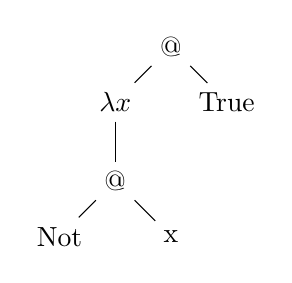
\begin{tikzpicture}
  \node(app) {@};
  \node(lambdax) [below left of=app]{$\lambda x$};
  \node(arg) [below right of=app]{True};
  \node(app2) [below of=lambdax] {@};
  \node(f) [below left of=app2] {Not};
  \node(x) [below right of=app2] {x};
  \draw (app) -- (lambdax);
  \draw (app) -- (arg);
  \draw (lambdax) -- (app2);
  \draw (app2) -- (f);
  \draw (app2) -- (x);
\end{tikzpicture} & 

$\rightarrow_{\text{xform}}$ &

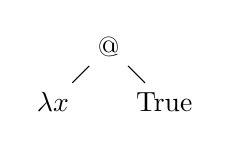
\begin{tikzpicture}
  \node(app) {@};
  \node(f) [below left of=app]{$\lambda x$};
  \node(arg) [below right of=app]{True};
  \draw (app) -- (f);
  \draw (app) -- (arg);
\end{tikzpicture}
\end{tblr}

$\iff$

($\lambda$x.Not x) True $\rightarrow$ (Not True)

sharing of redex and lambda abstraction: create new instances and do modification on those

large arguments: use pointers instead when doing substitution to formal parameters

rewrite root of redex with result ensures expressions shared are reduced only once

subcomponents of redex may be detatched afterward from the graph for garbage collection

reduction step reduces expression to a simpler one:
\begin{itemize}
\item but number of nodes in graph may not decrease due to nodes representing body of a function are introduced when applying a function
\item substitution of a subgraph referred by a function name with its definition
\end{itemize}

graph reducer code gen:
for each function in program
\begin{itemize}
  \item generate:
    \begin{itemize}
    \item function descriptor
    \item instructions, that will create the graph in memory corresponding to RHS definition of the function, when run
    \end{itemize}
  \item translate each core construct into a function call (instructions)
    \begin{itemize}
      \item identifiers: use its name,; no-op
      \item numbers and data: alloc on heap with contructor function
      \item function application: construct graph with application nodes and pointers to argument expressions
  \end{itemize}
\end{itemize}
  

\subsection{Preserving Original Lambda Abstraction for Reuse by Other Parts of the Program}
create a new instance of its body when the abstraction is used

detatch the template lambda abstraction from local graph after instantiation

eg, use a helper utility:
\begin{lstlisting}
instantiate(Body, Var, Value) $\equiv$ Body[Value/Var]
\end{lstlisting}

recursive function: apply case analysis for how to apply substitution to lambda abstraction

\subsection{Lazy Graph Reduction}
eval by need: use normal order evaluation to get WHNF $\implies$ arguments to function eval'd only if they are needed

eval same expression only once:
\begin{itemize}
\item substitute pointers instead of raw arguments to formal parameters $\implies$ deduplicate unevaluated arugment
\item update redex root with result $\implies$ evaluated redex cached for future uses to deduplicate works of re-evaluating
\end{itemize}

\subsection{Reduction of Application with Builtin Function}
\begin{enumerate}
\item recursively eval arguments by evaluator and reset root of redex to current redex under consideration
\item eval function
\item replace root of redex with result
\end{enumerate}

\subsection{Indirection Nodes}

\begin{itemize}
\item unboxed objects update
\item update where body of lambda abstraction is a single variable
\end{itemize}

a solution to indirection such that no sharing is lost: eval result to WHNF before updating root of redex

using indirection node to result vs. copying root of result of root of redex in the case of the root of result is not constructed during reduction
\begin{itemize}
\item needed if result if unboxed object
\item no issue if root of result is bigger than root of redex
\item but need additional tests for indirectionality and deref as they are encountered leading to slowness
\end{itemize}

\subsection{Impl. of Y Combinator}
by definition:

\begin{lstlisting}
  T f $\rightarrow_{\text{reduces to}}$ f ( Y f)
\end{lstlisting}

possible approaches:

\begin{tblr}{ccc}
\begin{tikzpicture}
  \node(app) {@};
  \node(f) [below left of=app]{Y};
  \node(arg) [below right of=app]{f};
  \draw (app) -- (f);
  \draw (app) --  (arg);
\end{tikzpicture} &
$\rightarrow$ &
\begin{tikzpicture}
  \node(app) {@};
  \node(f) [below left of=app]{f};
  \node(app2) [below right of=app]{@};
  \node(f2) [below left of=app2]{Y};
  \node(arg) [below right of=app2]{f};
  \draw (app) -- (f);
  \draw (app) -- (app2);
  \draw (app2) -- (f2);
  \draw (app2) -- (arg);  
\end{tikzpicture}
\end{tblr}

or

\begin{tblr}{ccc}
\begin{tikzpicture}
  \node(app) {@};
  \node(f) [below left of=app]{Y};
  \node(arg) [below right of=app]{f};
  \draw (app) -- (f);
  \draw (app) --  (arg);
\end{tikzpicture} &
$\rightarrow$ &
\begin{tikzpicture}
  \node(app) {@};
  \node(f) [below left of=app]{f};
  \draw (app) -- (f);
  \draw[->] (app) to [out=315, in=45, looseness=5] (app);
\end{tikzpicture}
\end{tblr}

2nd approach wuth cyclic graph:
\begin{itemize}
\item con: cycle is an potential issue for GC with ref counting
\item pro: use finite representation in storage to represent infinite object (recursive function, infinite data structure)
\end{itemize}

\vfill\null
\columnbreak

\section{FP: Supercombinator}

goal: transform lambda expression into a form such that lambda abstractions are easier to instantiate

a possible approach via lambda lifting where lambda abstractions are transformed into supercombinators

\subsection{Combinator}
definition: a lambda expression which contains no occurences of free variable (eg: a pure function)

supercombinators(further restrictions on top of being combinators) $\in$ combinators $\in$ lambda expressions

previously, instantiation done through recursive tree walk over over the lambda body

alternative: compilation to a fixed sequence of instructions to construct instance of lambda body $\implies$ instantiation of lambda body becomes following instruction sequence associated with it

dealing with free variables in lambda body:
\begin{itemize}
\item access values of free variables via environment by code sequence associated with the lambda abstraction
\item alternative: transform program where lambda abstractions can be easily compiled $\implies$ does not require additional environment
\end{itemize}

modified $\beta$-reduction by perform serveral $\beta$-reductions at once:
\begin{itemize}
\item less intermediate structure generated
\item following algo. of performing normal order reduction until WHNF is reached $\implies$ no work can be done on inner lambda abstraction until it is given another argument
\end{itemize}

\subsection{Supercombinator}

lambda expression of the form:
\begin{lstlisting}
$\lambda$x$_1$. .. $\lambda$x$_n$.E
\end{lstlisting}
where
\begin{itemize}
\item n $\geq$ 0
\item E is not a lambda abstrction
\item no free variables exist
\item any lambda abstraction in E is a supercombinator
\end{itemize}

amenable for multi-argument reduction

\subsection{Supercombinator of Arity $n>0$}
unit of compilation

no free variables $\implies$ can compile a fixed code sequence

any lambda abstraction in body have no free variables $\implies$ no copying when instantiating supercombinator body

\subsection{Supercombinator of Arity 0 / Constant Applicative Form}

known as CAF

can still be a function

no free variables and no $\lambda$s at front $\implies$
\begin{itemize}
\item never instantiated
\item  no code need to be compiled
\item 1 instance of its graph can be shared
\end{itemize}

\subsection{Supercombinator Creation}

represent a program with:
\begin{itemize}
\item a set of supercombinator definitions
\item an expression to be evaluated
\end{itemize}

supercombinator reduction takes place when all required arguments are present

implementation aspects:
\begin{itemize}
\item algo. to translate all lambda abstractions into supercombinators, eg: lambda lifting
\item an implemenation of supercombinator reduction
\end{itemize}

\subsection{Lambda Lifting}

make each free variable into an extra parameter (abstracting free variable) $\iff$ $\beta$-abstraction (inverse of $\beta$-reduction)

eg:

\begin{lstlisting}
($\lambda$y. + y x) $\Rightarrow$ ($\lambda$w.$\lambda$y. + y w) x
\end{lstlisting}

supercombinator notation:
\begin{lstlisting}
$\textdollar$F = $\lambda$W.$\lambda$Y. + Y W
$\Leftrightarrow$ $\textdollar$F W Y = + Y W (shorthand form)
\end{lstlisting}
where \verb|$F| is an arbitrary unique name given to a supercombinator

select a lambda abstraction, where there is no inner lambda abstractions in its body, to transform to supercombinator

apply this algo. until there is no more lambda abstractions

in the final form of the transformed program, the expression has no free variables since it is a top level expression $\implies$ make it a CAF (0-parameter supercombinator)

eg:

\begin{lstlisting}
original program:
($\lambda$x.$\lambda$y. - y x) 3 4

supercombinator definitions:
$\textdollar$XY x y = - y x
..
$\textdollar$Prog = $\textdollar$XY 3 4
---
top level expression:
$\textdollar$Prog
\end{lstlisting}

$\eta$-reduction of supercombinator difinitions may eliminate redundant definitions and this leads to smaller supercombinator definition set in replacements in expression

order parameters such that parameters corresponding to deeper nested lambda abstraction are put towards the back of parameter list $\implies$ makes $\eta$-reduction possible
\begin{itemize}
\item compute level number of lambda abstraction using textual nesting level: current level is number of surrounding lambda abstractions plus one
\item top level constants including supercombinators are defined to have a level of 0
\end{itemize}

impl. of compiling supercombinator body can use techniques from previous sections with graphs; jno free variables $\implies$ never need to be copied; substitution with multiple variables at once

alternatively represent body of supercombinator with a sequence of code only (no environment necessary) $\implies$ instantiation of supercombinator body corresponds to running the code sequence

\vfill\null
\columnbreak

\section{FP: Recursive Supercombinators}

extend body of supercombinator to have general graph

\begin{itemize}
\item \verb|letrec| expressions for representing cyclic body and infinite data structures
\item \verb|let| expression for acyclic body
\end{itemize}

\subsection{Transforming recursive program into supercombinator with graphical bodies}

assign lexical level numbers to variables bound in \verb|letrec|
\begin{itemize}
\item variable instantiated when immediate textually enclosing lambda abstraction is applied to an argument (when we construct instance of letrec, substituting for all free variables)\\
  $\implies$ variable bound in a letrec given lexical level number of immediately enclosing lambda abstraction

\item if no enclosing lambda abstraction, assign level number of 0
\item no free variables $\implies$ use lambda lifting to remove inner lambdas and transform into supercombinator
\end{itemize}

\vfill\null
\columnbreak

\section{FP: Fully Lazy Lambda Lifting}

\begin{itemize}
\item share dynamically created constant epressions
\item each expression evaluated at most once after variables in it have been bound
\end{itemize}

\subsection{Maximal Free Expressions}

\subsection{Formal Definition}
maximal free expression of a lmabda abstraction L $\equiv$
\begin{itemize}
\item all variables in expression are free
\item the expression is not a proper subexpression of another free expression of L
\end{itemize}

issue: laziness lost if too much of body of lambda abstraction is instantiated

determine what parts should not be instantiated: parts of the body that contain no free occurences of formal parameter $\implies$ that subexpression is invariant accross all instantiations, therefore can use 1 instance and share it

duing $\beta$-reduction, do not instantiate maximal free expressions of lambda abstractions; point to a single shared instance in the body of lambda abstraction

\subsection{Fully Lazy Lambda Lifting}

modify lambda lifting algo. such that impl. of the resulting supercombinator program is automatically fully lazy: abstract maximal free expressions when doing lambda lifting of a lambda abstraction instead of abstracting only free variables of lambda abstraction as extra parameters

when maximal free expression has no free variables in it (CAF) $\implies$ give it a name and make it into a supercombinaor instead of abstracting it as an extra parameter; given name used instead of the expression

2 phases:
\begin{itemize}
\item float \verb|letrec| and \verb|let| definitions out as far as possible
\item perform fully lazy lambda lifting
\end{itemize}

use a variable's set of free variables that the variable depends on\\
$\implies$ float the variable outwards until the next enclosing lambda abstraction binds 1 of the variables in the variable's free variable set\\
$\implies$ if no free variables at all, then variable/definition floated out to top level and turned into supercombinator

\subsection{Implementing Fully Lazy Lambda Lifting}

use lexical level number of expressions in addition to that of variables

lexical level of expression $\equiv max_i(\text{lexical level of } i), \forall i \in \text{free variables in expression}$ 

when lambda lifting a lambda abstraction at level n, all expressions within the body, that have levels less than n, are taken out as extra parameters

level number of any constant = 0 by definition

level number of a variable is the textual nesting depth of lambda which binds it

level number of an application \verb|(f x)| is the maximum of the level numbers of f and x

expression's native lambda abstraction $\equiv$ the 1st lambda abstraction which binds any variable in the expression; the enclosing lambda abstraction of the expression where level number is the same as that of the expression

implementation in a single tree walk over the expression:
\begin{enumerate}
\item traverse down the tree, record the level number of each lambda abstraction
\item on the way back up of the traversal, compute the level number of each expression by using the environment and level number of the expression's subexpressions
  \begin{itemize}
  \item in application of expression, if the level numbers are the same then two expressions are merged, if not they are given new unique names (they will be maximal free expressions of distinct lambda abstractions)
  \item merging mechanism $\implies$ forming maximal free expressions
  \end{itemize}
\item on way back up the traversal, from smaller free expressions encountered, lambda is transformed into supercombinator; lambda abstraction is replaced by supercombinator applied to maximal free expressions (subexpressions with level number less than that of the lambda abstraction after merging)
\end{enumerate}

lifting CAFs alternative:
\begin{itemize}
\item define a new supercombinator of 0 arguments
\item use the defined supercombinator in place of the oringal expression
\item constant expression with a single constant $\implies$ leave it since there is no additional benefit of liting it
\end{itemize}

reordering parameters of supercombinator in increasing level number
\begin{itemize}
\item maximize $\eta$-reduction opportunities
\item useful for maximal free expression parameters as well (take out smaller number of larger free expressions)
\end{itemize}

\subsection{float definitions given in let and letrec outward}

in order to have full laziness

assumes that dependency analysis of let(recs) have already been performed earlier, or else some definitions may not be floated out as outward as possible

impl. may possibly combined this phase with dependency analysis step

an algo:
\begin{itemize}
\item immediately enclosing lambda abstraction has the same level number as that of the variables bound in let(rec)
\item let(rec) is not present in function portion of an applicatoni
\item let(rec) floated out as little as possible subject to above constraints $\implies$ enable optimization of unreachable code
\end{itemize}

more concrete algo:
\begin{enumerate}
\item compute level numbers of each definition body $\implies$ needed for computing level number of variables that are bound to it
\item for letrec, assume level number of variables defined in letrec is 0 (level \# of recursive definition depends only in its free variables and not on level \# of recursive definition)
\item for letrec, compute maximum of level numbers of definitions' bodies $\implies$ this is the level \# for variables bound in letrec\\
  for let, level \# is computed in previous step (level \# of definition body)\\
  $\implies$ use this computed \# for variables bound in let(rec)
\item float out definitions up until the next enclosing lambda abstraction has the same level \# as that of variables defined in let(rec) computed in previous step
\item let(rec) appears in function position of an application $\implies$ continue to float it to next outer level
\end{enumerate}

note: letrec rebinds a variable already in scope $\implies$ cannot be floated outward unless renaming of variables is done (to avoid capturing occurences of outer variables)

situations where fully lazy lambda lifting does not gain improvements: selectively apply ordinary lambda lifting instead of fully lazy version
\begin{itemize}
\item builtin operator or supercombinator applied with too few arguments $\implies$ no eval takes place anyways so extra work to abstract out expressions is not worth it
\item arguments of function may be considered for abstraction
\item constant expressions (candidates for new supercombinator definition) do not gain much from abstracting them out since they are irreducible anyways
\end{itemize}

\subsection{general rules}
lambda abstraction \verb|\x.E| in a context that cannot be shared\\
$\implies$ do not abstract free expressions from E because they will not be shared\\
$\implies$ only abstract free variables

justifications:\\
free expressions in E are not shared outside of E by definition\\
free expressions in E are not shared inside E since they are abstracted from a single place in E

in the above way, lambda lifting algo. becomes context dependent

figuring out if a lambda abstraction may be shared is difficult in general, but we may give up at any time and assume partial applicatoin may be shared

\vfill\null
\columnbreak

\section{FP: SK Combinators}

\begin{lstlisting}
S f g x = f x g(x)
K x y = x
I x = x
\end{lstlisting}

extensional equality

compile-time transformations with S, K, I:
I-transformation:
\begin{lstlisting}
$\lambda$x.x $\implies$ I
\end{lstlisting}

K-transformation
\begin{lstlisting}
$\lambda$x.c $\implies$ K c
\end{lstlisting}

S-transformation:
\begin{lstlisting}
$\lambda$x.e$_1$ e$_2$ $\implies$ S ($\lambda$x.e$_1$)($\lambda$x.e$_2$)
\end{lstlisting}

use of S, K, I to compile any lambda abstraction to expression with S, K, I terms and constants; other variables disappear

basic algo.:
\begin{lstlisting}
while expr. contains a lambda abstraction, then:
  choose an innermost lambda abstraction in expr.
  body of the lambda abstraction is:
    application $\Rightarrow$ apply S-transformation
    variable/constant $\Rightarrow$ apply K or I transformation
\end{lstlisting}

recursion $\implies$ use Y-combinator; Y is treated as a builtin function by the combinator compilation algorithm

\subsection{SK Compilation Algo.}
\begin{lstlisting}
C[[ e$_1$ e$_2$ ]] = C[[ e$_1$ ]] C[[ e$_2$ ]]
C[[ $\lambda$x.e ]] = A x [[ C[[ e ]] ]]
C[[ cv ]] = cv
A x [[ x ]] = I
A x [[ cv ]] = K cv
A x [[ f$_1$ f$_2$ ]] = S (A x [[ f$_1$ ]]) (A x [[ f$_2$ ]])

where:

cv $\equiv$ a constant / builtin function
x $\equiv$ a variable
f$_i$ $\equiv$ expr. without any inner $\lambda$s
e$_i$ $\equiv$ expression
\end{lstlisting}

note: C applied to body of lambda before applying A $\implies$ all inner lambdas are dealt with; A only has to deal with atoms and applications

\subsection{K Optimization}

fewer reductions, enable more laziness

\begin{lstlisting}
S (K p) (K q) $\Rightarrow$ K (p q)
\end{lstlisting}

when body of lambda abstraction does not use parameter of lambda:
\begin{lstlisting}
A x [[ e ]] = K e $\iff$ x not used in e
\end{lstlisting}

\subsection{B Combinator}

\begin{lstlisting}
S (K p) q $Rightarrow$ B p q $\equiv$ $\lambda$x.p (q x)

where:

B f g x = f (g x) //runtime reduction
\end{lstlisting}

useful when lambda abstraction only uses parameter in the right branch

\subsection{C Combinator}
\begin{lstlisting}
S p (K q) $\Rightarrow$ C p q $\equiv$ $\lambda$x.(p x) q

where:

C f g x = f x g
\end{lstlisting}

useful when lambda abstraction only uses parameter in the left branch

special case for \verb|S (K p) I| $\Rightarrow$ \verb|p|

\subsection{modification to SK compilation algo. using the above}

\begin{lstlisting}
A x [[ f ]] $\equiv$ abstracts x from f
---
A x [[ x ]] = I
A x [[ cv ]] = K cv
A x [[ f$_1$ f$_2$ ]] = S (A x [[ f$_1$ ]]) (A x [[ f$_2$ ]])
  $\Rightarrow$ Opt[[ S (A x [[ f$_1$ ]]) (A x [[ f$_2$ ]])

where:

Opt[[ S (K p) (K q) ]] = K (p q)
Opt[[ S (K p) I ]] = p
Opt[[ S (K p) q ]] = B p q
Opt[[ S p (K q) ]] = C p q
Opt[[ S p q ]] = S p q
\end{lstlisting}

\subsection{S' Combinator Optimization}
for compiling
\begin{lstlisting}
$\lambda$x$_n$ .. $\lambda$x$_1$.p q where p and q both use x$_n$ .. x$_1$
\end{lstlisting}

let:
\begin{lstlisting}
S' c f g x = S (B c f) g x
  $\rightarrow$ (B c f) x (g x)
  $\rightarrow$ B c f x (g x)
  $\rightarrow$ c (f x) (g x)
\end{lstlisting}

then:

\verb|S' c f g x = c (f x) (g x)|

$\implies$

\begin{lstlisting}
p q
= S $^1$p $^1$q
= S' S $^2$p $^2$q
= S' (S' S) $^3$p $^3$q
...
= S' (S' (..(S' S)..) ) $^n$p $^n$q //n-1 times of S'

where:

$^1$p = A x$_1$ [[ p ]]
$^2$p = A x$_2$ [[ $^1$p ]]
...
\end{lstlisting}

\verb|O(n)| expansion complexity

analogous B' and C' combinators for abstracting many variables used only in p or q but not both

\begin{lstlisting}
B' c f g x $\rightarrow$ c f (g x)
C' c f g x $\rightarrow$ c (f x) g

compilation rules:

B (c f) g $\Rightarrow$ B' c f g
C (B c f) g $\Rightarrow$ C' c f g
\end{lstlisting}

eg:

\begin{lstlisting}
C (B c f) g x = (B c f x) g
              = c (f x) g  
\end{lstlisting}

further optimization for B':

\begin{lstlisting}
B c (B f g) $\Rightarrow$ B$^*$ c f g

where:

B$^*$ c f g x $\rightarrow$ c(f(g x))
\end{lstlisting}

\subsection{Final SK Compilation Algo.}
\begin{lstlisting}
Opt[[ e ]] optimizes e
---
Opt[[ S (K p) (K q) ]] = K (p q)
Opt[[ S (K p) I ]] = p
Opt[[ S (K p) (B q r) ]] = B$^*$ p q r = $\lambda$x.p(q(r x))
Opt[[ S (K p) q ]] = B p q
Opt[[S (B p q) (K r) ]] = C' p q r = $\lambda$x.p (q x) r
Opt[[ S p (K q) ]] = C p q
Opt[[ S (B p q) r ]] = S' p q r = $\lambda$x.p (q x) (r x)

where:

I x $\rightarrow$ x
K c x $\rightarrow$ c
S f g x $\rightarrow$ f x (g x)
B f g x $\rightarrow$ f (g x)
C f g x $\rightarrow$ (f x) g = f x g
S' c f g x $\rightarrow$ c (f x) (g x)
B$^*$ c f g x $\rightarrow$ c(f(g x))
C' c f g x $\rightarrow$ c(f x) g
\end{lstlisting}

\vfill\null
\columnbreak

\section{FP: G Machine}

compiling supercombinators to G-code

compilation scheme F:

\begin{lstlisting}
F[[ $\textdollar$G x$_1$ .. x$_n$ = E ]] = G-code for $\textdollar$G
\end{lstlisting}

use of graph and stack for evaluation

auxilliary R compilation scheme to compile body, E, of supercombinator:
\begin{lstlisting}
R[[ E ]] p d

where:

p: maps identifier to offset of the argument from
   the base of the current context
d: depth of current context - 1
R: create instance of body of supercombinator using
     parameters on the stack
   update root of redex with copy of root of result
   remove parameters from the stack
   initiate next reduction
\end{lstlisting}

C compilation scheme:

constructs code/instructions for generating an instance of a target expression

args: expression for compilation; p and d: where arguments of supercombinator are found on the stack

result:
\begin{itemize}
\item code sequence that can construct instance of the expression
\item substitution of found parameters with supercombinator arguments that are referenced
\item a pointer to the instance on top of the stack
\end{itemize}

define \verb|C[[ E ]] p d| for each case of expression E

\begin{lstlisting}
C[[ i ]] p d = PushInt i
C[[ f ]] p d = PushBlobal f
C[[ x ]] p d = Push (d - p x) //copy to top of stack
C[[ E$_1$ E$_2$ ]] p d =
  C[[ E$_2$ ]] p d;
  C[[ E$_1$ ]] p (d+1);
  MakeAp
C[[ let x = E$_x$ in E$_b$ ]] p d =
  C[[ E$_x$]] p d;//create Ex instance on top of stack
  C[[ E$_b$]] p[x=d+1] (d+1);//create Eb on stack using
    instantiated pointer to Ex already on stack
  Slide 1;//discard associated item with Ex on stack
C[[ letrec D = E$_b$ ]] p d =
  CLetrec[[ D ]] p' d';
  C[[ E$_b$ ]] p' d';
  Slide (d'-d);//discard item associated with D on stack
    since it is referenced by Eb, while keeping item
    associated with Eb instance on top of stack

where:

i is a constant value or pointer to the value
f is a function
x is a variable; value is in the stack at offset
  (d - p x) from the top
MakeAp is an application cell that takes and pops
  2 items on stack and forms application node in
  the heap, puts a pointer to the node on top of
  the stack
p[x=y] a = y,   x = a
         = p a, x $\neq$ a
(p', d') = Xr[[ D ]] p d
CLetrec[[ x$_1$ = E$_1$
          ..
          x$_n$ = E$_n$ ]] p d =
  Alloc n;//create n holes in heap and pushes n
    pointers onto stack
  C[[ E$_1$ ]] p d; Update n;//construction of
    definition body instance; updates associated hole
    in heap with root of created instance of
    definition body
  ..
  C[[ E$_n$ ]] p d; Update 1
Xr[[ x$_1$ = E$_1$
     ..
     x$_n$ = E$_n$]] p d =
  (p[x$_1$ = d + 1
     ..
     x$_n$ = d + n], d + n) // augmentation of p and d
\end{lstlisting}

note: if definition body is a single varialb ename fou din the same letrec:
\begin{lstlisting}
letrec x = y
       ..
       y = Cons 1 y
\end{lstlisting}
then update will perform update 1 hole with another; avoid this by removing definition of x and replaceing with y at an earlier stage of compiler (elimination of  redundant lets where rhs of let is a single variable by replacing occurences of lhs variable with rhs variable in body of let)

\subsection{GC of CAFSs}
compiled version of code:
\begin{itemize}
\item need explicit list of references of directly/indirectly used CAFs since it is not apparent in compiled instructions
\item use of expicit list of CAFs (info given to GC implementation) that each supercombinator uses for marking (signal object is reachable from a root and cannot be eligeable for garbage collection) in GC sweeps
\end{itemize}

supercombinator with $\geq$ 1 argument(2) can't grow in size $\implies$ no need for GC

unreduced CAF marking $\implies$ mark its associated list of CAFs

reduced CAF marking $\implies$ like any other heap data structure for marking

supercombinator with $\geq$ 1 argument(s) marking $\implies$ mark all CAFs in its associated list

\subsection{Options for Compiling CAFs}
not compile:
\begin{itemize}
\item leave in graph form
\item never copied
\item shared
\item program may be a mixture of compiled code and graph
\end{itemize}

compile:
\begin{itemize}
\item supercombinator with 0 arguments
\item compile to G-code: code that will instantiate their graph when executed
\item instantiation will need to overwrite some code for sharing so that further use will not require repeated copied of it; possible impl:
  \begin{itemize}
  \item code alloc. a graph node representing a function (a pointer to compiled code)
  \item execution of compiled code updates the graph node (1 per supercombinator; not in read only memory since it needs to be updated when code is executed) associated with it with the result; the result is sharable with other users through the shared graph node
  \end{itemize}
\end{itemize}

\subsection{Builtin Function}

translation to G-code sequence:
\begin{itemize}
\item eval to WHNF whenever possible to eliminate duplicate work
\item UNWIND vs. RETURN instruction
\item PUSH
\item EVAL
\item UPDATE
\item POP
\item SELSUM$_{r,i}$
\item SELPRODUCT$_{r,i}$
\item JUMP
\item JFALSE
\item CASEJUMP$_{StructTag, n}$
\end{itemize}

\vfill\null
\columnbreak

\section{FP: Abstract Machine Model Describing G-Code}

machine state: \verb|<S,G,C,D>|\\
S: stack\\
G: graph\\
C: code sequence (G-code)\\
D: dump / stack of \verb|(stack, code sequence)|

operation of G-machine $\iff$ state transition, eg:

\begin{lstlisting}
<S, G, PushInt i: C, D $\Rightarrow$
  <n:S, G[n=Int i], C, D>

<n: S, G[n = Ap n$_1$ n$_2$], Eval: C, D> $\Rightarrow$
  <n:[], G[n = Ap n$_1$ n$_2$], Unwind:[], (S,C): D>

// will eventually update the CAF function node with
//   result of reduction
<n: S, G[n = Fun 0 C'], Eval: C, D> $\Rightarrow$
  <n:[], G[n = Fun 0 C'], C':[], (S,c): D>

<n: S, G[n = Int i], Eval: C, D> $\Rightarrow$
  <n: S, G[n = Int i], C, D>

where:

n: a unique new name
\end{lstlisting}

non-existent transition $\implies$ runtime error

cases for transition of Unwind:

item on top of stack:
\begin{itemize}
\item Cons or Int node $\implies$ WHNF; only item in current stack; restore saved stack and code from dump; put result on top of the restored stack
\item pointer to application node $\implies$ push head of application on stack; repeat Unwind instruction
\item a function with enough arguments on stack $\implies$ rearrange stack; execute code for the function
\item a function without enough arguments $\implies$ expression under eval is in WHNF; restore saved stack and code from dump; put result of eval on top of restored stack
\end{itemize}

\subsection{Printing Mechanism}

need an evaluator invocation mechanism that reduce expressions to WHNF and also print them

add an additional compone tin G-machine state, O

add a Print instruction: print element on top of the stack

eg:

\begin{lstlisting}
<O, n:S, G[n = Int i], Print:C, D> $\Rightarrow$
  <O:i, S, G[n = Int i], C, D>

<O, n:S, G[n = Cons n$_1$ n$_2$], Print:C, D> $\Rightarrow$
  <O, n$_1$:n$_2$  :S, G, Eval:Print:Eval:Print:C, D>

<O, n:S, G[expr], i:C, D> where i $\neq$ Print $\Rightarrow$
  O is unchanged
\end{lstlisting}

\verb|Begin| instruction initializes the G-machine:

\begin{lstlisting}
<O, S, G, Begin:C, D> $\Rightarrow$ <O, [], [], C, []>
// note: empty stack, graph, dump
// and runs rest of the code C
\end{lstlisting}

\subsection{Impl. of G-code}
compute memory space required by each supercombinator and insert instructions to check for sufficient memory (heap) at beginning of function (do at compile with a simulated model of stack)

simulated stack expected to be empty at the end of the execution of a supercombinator

eval may cause arbitrary amount of computation to occur

issue: possible GC interruption disturb simulated stack and heap

possible solution for when flow of control can be broken
\begin{itemize}
\item segments of code between Evals has its own code to check for heap exhaustion $\implies$ simulated stack and heap pointers/offsets calculated relative to EP(stack pointer) and HP(heap pointer) at beginning of each code segment (not necessarily start of each supercombinator)
\item before Eval is called, simulated stack is flushed oto the real stack
\item also apply this separate code segment technique to code with JUmp instructions:
  \begin{itemize}
  \item different routes due to different branches may have different amounts of heap allocated and simulated stacks are different
  \item simulated stack flushed to real stack before Jump
  \end{itemize}
\end{itemize}

dealing with graphs via an interface to be used from G-code execution mechanism; types of graph operation:
\begin{itemize}
\item node specific operation, when node being evaluated is known to be of that type
\item generic operation: eval on unknown node; usually need case analysis on node type $\implies$ more expensive
\end{itemize}

tag case analysis:
\begin{itemize}
\item tag in a cell points to a table of code entry points (one entry point per generic operation)
\item different node type associates with different entry table
\item possible use of cell/boxed values to achieve a unifrom case analysis for different typed nodes
\item use of indireciton node instead of copying root of result of reduction into root of the redex
\item Unwind G-code instruction:
  \begin{itemize}
  \item WHNF: return to caller
  \item function with enough args: rearrange stack to prep for actual invocation of function's code
  \end{itemize}
\item Unwind on application call: push head of cell on stack and Unwind again
\item Eval code:
  \begin{itemize}
  \item code generated for Eval G-code instr., then
  \item call eval code in an entry of an entry table associte with the node tpye via a subroutine jump instr.
  \item cell type:
    \begin{itemize}
    \item WHNF (eg: primitive/function cell/ Cons cell): return from subroutine
    \item App cell/node: push current stack on dump (system stack) and call Unwind on application
    \end{itemize}
  \end{itemize}
\end{itemize}

per supercombinator:
\begin{itemize}
\item Globstart: Unwind code, GC code, entry table, function node via instr. to alloc. it at start of function code, overflow checking code preceding target code for function body
\item target functinon code
\end{itemize}

Begin: initialize stack and heap for entire system and other system specific tasks

End: terminate execution of whole program

\vfill\null
\columnbreak

\section{FP: Optimizations to G Machine}

avoid heap allocation / avoid huilding graphs

try use cheaper stack to cut allocation

laziness preservation for R compilation scheme (code generation for: applying a supercombinator to its arguments)

case analysis for each kind of expression for R compilation scheme:
\begin{lstlisting}
R[[ i ]] p d =
  PushInt i;
  Update (d+1);
  Pop d;
  Return //not Unwind since Int can't be applied

R[[ f ]] p d =
  PushGlobal f;
  Eval; //needed for the case of reduction of CAF
  Update (d+1);
  Pop d;
  Unwind

//for the case of body being a single variable
//  load value onto stack; eval it;
//  update result of reduction into root of redex
R[[ x ]] p d =
  Push (d - p x);
  Eval;
  Update (d+1);
  Pop d;
  Unwind

R[[ E$_1$ E$_2$ ]] p d =
  C[[ E$_1$ E$_2$ ]] p d;
  Update (d+1);
  Pop d;
  Unwind

R[[ let x = E$_x$ in E ]] p d =
  C[[ E$_x$ ]] p d;
  R[[ E ]] p[x = d+1] (d+1)

R[[ letrec D in E ]] p d =
  CLetrec[[ D ]] p' d';
  R[[ E ]] p' d'
  where (p'd') = Xr[[ D ]] p d
\end{lstlisting}

direction execution of builtin functions instead of building a graph and immediately unwinding it

optimize code for special cases for \verb|C[[ E ]] p d; Eval| sequence:

\verb|E[[ E ]] p d| generate G-code which eval.(equivalent C-eval sequence) E to WHNF and leave result on top of the stack (replace occurences of C-eval sequence in R scheme with E compilation scheme)

RS sceheme, ES scheme: enable E scheme optimization

\subsection{$\eta$-reduction and lambda lifting}
\begin{itemize}
\item may incur cost during code generation
\item perform only if it eliminates an entire function definition
\item eg: \verb|(f E1 E2 ..)| if \verb|f| is unknown such as ones passed into function as argument, then optimzed code generation is less likely
\end{itemize}

\subsection{Fatbar and Fail}
optimize by never producitng a Failure value and replace it with instructions

\subsection{Evaluating arguments}

if function is strict in an argument, then it's safe to use E scheme and avoid building a graph before eval it

partial application / supercombinator that return a function: eval provided arguments straight away instead of building graphs

\subsection{Strictness Analysis}
propagate strictness info. bottom up

use a map: \verb|(function, arg_position) -> bool|

base cases:
\begin{itemize}
\item parameter/ local variable in letexpr $\implies$ strict identifiers set: \verb|{var}|
\item constant / data constructor / function names $\implies$ empty strict identifiers set
\end{itemize}

construct and strictness propagate rules
\begin{itemize}
\item \verb|L op R| $\implies$ L $\cup$ R
\item \verb|if C then T else E| $\implies$ C $\cup$ (T $\cap$ E)
\item fun$_m$ @ $A_1$ .. $A_n$ $\implies$ $\cup$ strict(fun.i)$_{i=1}^{min(m,n)}$ A$_i$, n $\geq$ m
\item F @ $A_1$ .. $A_n$ $\implies$ F
\item let v= V in E $\implies$ (E $\backslash$ \{v\}) $\cup$ V, v $\in$ E\\
  let v= V in E $\implies$ E, v $\not\in$ E
\end{itemize}

recursive function
\begin{itemize}
\item assume optimistic initial set
\item propagate and compare result set to initial assumption
\item repeat propagate with updated assumption until the result agrees with assumption
\item in the degenerate case of recursive function that does not terminate, optimistic scheme reports strict arguments that are actually not strict; in practice it's not a serious issue anyways
\end{itemize}

analysis of strictness of data structure is hard in general, many analyzers not address this

use of programmer annotation / manually indicating strictness, eg: seq in Haskell

can use strictness info. for optimization, eg: to avoid creating application nodes and spines

\subsection{Global Strictness Info}

using strictness analysis:
\begin{itemize}
\item annotate application of functions that are strict wrt. parameters
\item annotate definitions and application nodes
\end{itemize}

eg: an infix op \verb|!| denoting strict applciation and strict let expression:

\verb|$F ! x = ..| where F is strict in x

acheives similar effect as call by value

avoid Eval to reduce cost (in G-machine instr. set):
\begin{itemize}
\item avoid re-evaluation in function body:\\
  track context info about whether item on a stack has been evaluated or not (eg: stack position -> Bool)\\
  also modify compilation schemes to return modified env. in addition to the generated code as before
\item supercombinator begins with code to Eval for each argument that the function is strict on
\item no-eval version of the function called after strict arguments are eval'd in the supercombinator 
\end{itemize}

avoid repeated unwinding:
\begin{itemize}
\item add info on arugments' evaluation status (WHNF or not)\\
  eval function if it is passed as a strict argument instead of deferring when function is applied
\item add a tag indicating WHNF for application node $\implies$ Eval entry for AP-WHNF's entry table is an immediate return instead of Unwind and finding function at tip of spine graph has too few arguments (eg: in WHNF) before returning;\\
  modify C scheme for compiling application of a function to too few arguments
\item all vertebrae below the root of redex at completion of Unwind instruction are then in WHNF because each represents application of a function to too few number of arguments;\\
  tags on these vertebrae can be changed to AP-WHNF as they are rearranged / removed from the stack as Unwind completes
\end{itemize}

\subsection{Eager Evaluation}
\begin{itemize}
\item avoid creating cells and application spines to unwind when evaluating expressions
\item specialize C scheme to directly use code instead of creating cells
\item if arguments is known to be eval'd already, then avoid extr cell creation and use direct code for eager eval $\implies$ performs operations that may not be used (graph created with C scheme may be discarded)\\
  $\implies$ this is still safe since the arguments are for sure already evaluated so it will terminate\\
  $\implies$ still usually faster than allocating cells on the heap
\item propagate this info. upward via environment which records items on stack being already evaluated or not
\end{itemize}

\subsection{Boxing Analysis}

applied after strictness analysis

finds which arguments ar esuitable for unboxing

pass basic value unboxed at strict argument positions

temporary/transient cells and bitmasking instr. may be used in boxing/unboxing in between other operations that are costly

instructions to:
\begin{itemize}
\item support operations on naked values
\item fox and unbox values on top of stack (cells in heap)
\item modify associated compilation scheme to support this
\end{itemize}

need modification for GC system to distinguish box vs. unboxed items on stack
\begin{itemize}
\item eg: can use an additional stack for only unboxed values and instructions are aware which stacks to use based on unboxed/voxed form of tiem
\end{itemize}

\subsection{Pointer Tagging}
use alignment constraints of addresses to stor additional info. in a few bits to discriminate things like boxed vs. unboxed values

mask/unmask bits before using actual pointer

\subsection{Vector Apply Node}
instead of binary application node, use: function pointer + length field + n argument pointers

unwinding skipped and reducer directly invoke function since vector apply node is already a closure with needed arugments inside (assuming nuber of args match arity of function)

normally unwinding application node via stacking arguments before invoking function via code address

\subsection{Peephole Optimization}

sits in between G-code compiler and code generator

replace short consecutive sequence of G-code instr. with more optimal sequence (instr. compression)

eg:

\verb|MKAP n|, \verb|SLIDE n|

if f is a builtin/supercombinator with $\geq$ 1 arguments: eliminate Eval instruction:
\begin{lstlisting}
// if f is not a CAF
PushGlobal f; Eval $\Rightarrow$ PushGlobal F 
\end{lstlisting}

build root of result directly on top of root of redex (to avoid allocating cell for result and copying result to root of redex)

use an instruction to use items on stack to build app node on top of root of redex
$\implies$ modify some compilation schemes for this:
\begin{itemize}
\item \verb|RS[[ f ]] p d n|
\item \verb|RS[[ x ]]|
\item \verb|CLetrec Schemes|
\end{itemize}

\subsection{Unpacking Structred Objects}
eg: present in lets compiled from case expressions

use a unpack instruction, eg: \verb|UnpackSum k|: unpacks top element on stack into k components (place them on top of the stack)

eg:

\begin{lstlisting}
let v$_1$ = SelSUm$_{k,1}$ v
    ..
    v$_k$ = SelSUm$_{k,k}$ v
in E

$\Updownarrow$

Push (d - p v); SelSum$_{k,1}$;
..
Push (d + k - 1 - p v); SelSum$_{k,k}$;

$\Downarrow$

Push (d - p v);
UnpackSum k;
\end{lstlisting}

Pattern Matching in a function is not compiled to:
\begin{enumerate}
\item code sequence to eval arg.
\item multiway jump based on structure tag of the argument
\item unpack instruction (take strucure apart and puts components on the stack)
\item code sequence to eval rhs. of the function (eg: free variables and components of structure in the stack)
\end{enumerate}

\vfill\null
\columnbreak

\section{FP: Generalized Tail Call Optimization}

squeeze out items on the stack associated with previous function before calling the tail function $\implies$ enable eliding extra instruction and space on stack needed for the function call

eg:

\begin{lstlisting}
C[[ E$_3$ ]] p d;
C[[ E$_2$ ]] p (d+1);
C[[ E$_1$ ]] p (d+2);
PushGLobal W;
Squeeze 4 2; //rid of F's 2nd and 1st args on stack
// at runtime, do case analysis on
// function on top of the stack
Dispatch 3 
\end{lstlisting}

Dispatch instruction is behaviourly equivalent as doing:
\begin{enumerate}
\item construct spine in heap from ribs on the stack
\item update root of the redex (bottom of current context) using the constructed spine
\item Unwind W
\end{enumerate}

case analysis of tail call:
\begin{itemize}
\item W is an Application node: in general, number of args W takes is unknown\\
  optimize construction of spine: do it on the stack instead of heap\\
  perform 1st part of Unwind as we construct the spine\\

  transition rule for Dispatch:

\begin{lstlisting}
<f:n$_1$:n$_2$:..:n$_k$:r:S,
  G[f = Ap m$_1$ m$_2$], Dispatch k:[], D>
$\Rightarrow$
<f:v$_1$:v$_2$:..:v$_{k-1}$:r:S,
  G[v$_1$=Ap f n$_1$;
    v$_i$ = Ap v$_{i-1}$ n$_i$, $i\in(1,k)$;
    r = Ap v$_{k-1}$ n$_k$],
  Unwind:[], D>
\end{lstlisting}

then, proceed to do as usual:
\begin{itemize}
\item construct spine of body of \verb|$F|
\item update root of \verb|$F_redex|
\item Unwind
\end{itemize}

\item W is a supercombinator and a CAP (0 args):
  Dispatch's behaviour same as if W is an application node (previous case)

\item W has exactly the number of args as the function requires: enter the code for W:
\begin{lstlisting}
<f: S, G[f = Fun k C], Dispatch k:[], D> $\Rightarrow$
  <S, G, C, D>  
\end{lstlisting}

entry into code for the function after arity check

\item W: number of provided args $\geq$ the arity of function parameters

  partial reduction of body of \verb|$F|: part of body of \verb|$F| becomes next redex

  construct a new context where W will execute in:
  \begin{itemize}
  \item W's args placed on top of the stack
  \item root of W-redex (placeholder hole to be later filled with the result of reduction of W) pointed to by an item in the stack below W's args
  \item construct top partial spine of the body of \verb|$F|
  \end{itemize}

\item W: number of available args $\leq$ number of parameters function requires

  body of \verb|$F| is then in WHNF

  need to update root of \verb|$F-redex|:

  \begin{itemize}

    \item construct spine in heap as in the case of an application node

    \item Dispatch should test depth of the stack to see if there are enough arguments after the spine is constructed and root of \verb|$F-redex| is updated:

      not enough args for W to reduce $\implies$  eval is complete; Dispatch initiates a Return

      enough args for W to reduce $\implies$ Dispatch rearranges the stack to prepare the call to W and finally enter W
    \end{itemize}

    \begin{lstlisting}
// eg, assuming W takes 4 arguments
stack:
---
root of W-redex -> v$_4$
root of F-redex -> r
n$_3$:E$_3$
n$_2$:E$_3$
n$_1$:E$_1$
f: W
..

// after arrangement by Dispatch
root of W-redex

stack:
---
root of W-redex -> v$_4$
n$_4$:E$_4$ -> n$_4$
n$_3$:E$_3$ -> n$_3$
n$_2$:E$_2$ -> n$_2$
n$_1$:E$_1$ -> n$_1$
    \end{lstlisting}
    
\begin{tblr}{ccc}
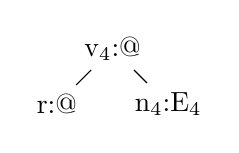
\begin{tikzpicture}
  \node(v4) {v$_4$:@};
  \node(a) [below left of=v4]{r:@};
  \node(b) [below right of=v4]{n$_4$:E$_4$};
  \draw (v4) -- (a);
  \draw (v4) -- (b);
\end{tikzpicture} &
$\rightarrow$ &
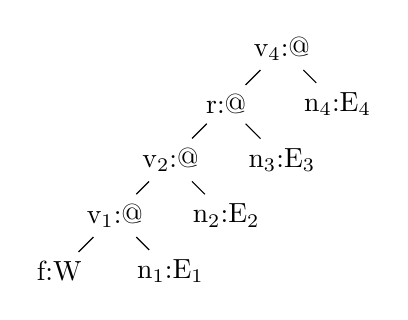
\begin{tikzpicture}
  \node(v4) {v$_4$:@};
  \node(r) [below left of=v4]{r:@};
  \node(v2) [below left of=r]{v$_2$:@};
  \node(v1) [below left of=v2]{v$_1$:@};
  \node(f) [below left of=v1]{f:W};
  \node(n4) [below right of=v4]{n$_4$:E$_4$};
  \node(n3) [below right of=r]{n$_3$:E$_3$};
  \node(n2) [below right of=v2]{n$_2$:E$_2$};
  \node(n1) [below right of=v1]{n$_1$:E$_1$};
  \draw (v4) -- (r);
  \draw (r) -- (v2);
  \draw (v2) -- (v1);
  \draw (v1) -- (f);
  \draw (v4) -- (n4);
  \draw (r) -- (n3);
  \draw (v2) -- (n2);
  \draw (v1) -- (n1);
\end{tikzpicture}
\end{tblr}

\end{itemize}

\subsection{transition rule for Dispatch when not enough arguments for function to reduce}

\begin{lstlisting}
<f:n$_1$:n$_2$:..:n$_k$:r:v$_{k+1}$:..:v$_d$:[],
  G[f = Fun a C], Dispatch k:[], (S, C'):D>
{k < d < a }
$\Rightarrow$
<v$_d$:S,
  G[v$_1$ = AP-WHNF f n$_1$
    v$_i$ = AP-WHNF v$_{i-1}$ n$_i$ (1<i<k)
    r = AP-WHNF v$_{k-1}$ n$_k$],
  C',
  D>  

where:

k: argument to dispatch
d: # of args available
a: arity of function on top of the stack
\end{lstlisting}

note:
\begin{itemize}
\item eval complete by making a return to the caller
\item vertebrae $v_i$s are in WHNF, thus construct them as type AP-WHNF nodes
\end{itemize}

\subsection{transition rule for the case of enough args. for the function to reduce}

rearrangement of stack happens

followed by jump to code of the function

\begin{lstlisting}
<f:n$_1$:..:n$_k$:r:v$_{k+1}$:..:v$_a$:S,
  G[f = Fun a C
    v$_{k+1}$ = Ap r n$_{k+1}$
    v$_i$ = Ap v$_{i-1}$ n$_i$, (k+1 < i $\leq$ a)],
  Dispatch k: [],
  D>
{k < a}
$\Rightarrow$
<n$_1$:..:n$_{k+1}$:..:n$_a$:v$_a$:S,
  G[v$_1$ = AP-WHNF f n$_1$
    v$_i$ = AP-WHNF v$_{i-1}$ n$_i$, (1<i<k)
    r = AP-WHNF v$_{k-1}$ n$_k$],
  C,
  D>
\end{lstlisting}


\subsection{Compilation using Dispatch}

modifications to RS scheme:

\begin{lstlisting}
RS[[ x ]] p d n =
  Push (d - p x);
  Squeeze (n+1) (d-n);
  Dispatch n

RS[[ f ]] p d n =
  PushGlobal f;
  Squeeze (n+1) (d-n);
  Dispatch n
\end{lstlisting}

\subsubsection{function is known at compile time}
perform case analysis at compile time to generate code instead of analysis at runtime

eg:

\begin{lstlisting}
PushGlobal $\textdollar$H;
Squeeze p q;
Dispatch k

where $\textdollar$H takes exactly k args

$\Rightarrow$

tail call case and generate code to jump to $\textdollar$H's code
(after arity check and stack rearrangement)
\end{lstlisting}


eg:
\begin{lstlisting}
PushGlobal $\textdollar$Cons;
Squeeze 3 q;
Dispatch 2;
$\Rightarrow$
Cons;
Update (q+1);
Pop q;
Return;
\end{lstlisting}

\subsubsection{other case}

\begin{lstlisting}
Push n;
Squeeze p q;
Dispatch k;
\end{lstlisting}

perform case analysis at runtime using G-code code generation using a Dispatch entry to each tag's entry table

eg:
\begin{lstlisting}
  moval 3, r2 //k parsed to Dispatch code via r2
  movl (%EP)+, r0 //pop function into r0
  movl r0, r1 //move tag into r1
  //do case analysis jump using offset to
  //Dispatch entry of entry table
  jmp * O_Dispatch(r1) 
\end{lstlisting}

\subsection{Optimizing E scheme}

apply similar optimization in RS scheme to ES scheme

allocate a hole to receive the result, then build ribs using ES scheme and push them on the stack

\begin{lstlisting}
E[[ E$_1$ E$_2$ ]] p d =
  Alloc 1;
  ES[[ E$_1$ E$_2$ ]] p d 0;

ES[[ x ]] p d n =
  Push (d - p x);
  Call n;

ES[[ f ]] p d n -
  PushGlobal f;
  Call n;

<f:n$_1$:..:n$_k$:r:S, G, Call k: C, D>
$\Rightarrow$
<f:n$_1$:..:n$_k$:r:[], G, Dispatch k: [], (S,C): D>
\end{lstlisting}

Call is like Dispatch except stack and code pointer are saved to the dump


\subsection{Comparison to Other Environment Based Implementations}

typical env. based impl:
\begin{itemize}
\item eval body of function in an environment (container that captures variable values in scope) where formal parameters are bound to their values
\item if the result of eval is a function-like object, then we return a closure (function's code pointer + environment in which the function will be executed in)
\item environment implementation: linked list or tuple consisting of only used values of variables that occur free in the body of the function
\end{itemize}

similarity to eng.cased impl:
\begin{itemize}
\item equivalent in G-machine: a graph with supercombinator aplpied to too few args.
\item extra args. produced from lambda lifting algo. to a function
\item execution in G-machine is based on stack (args found on stack) whereas env.-based impl. may access free variables (not present in supercombinator) in its environment
\item args passed to a function placed on stack before calling 
\end{itemize}

differences to env.-based impl.:
\begin{itemize}
\item enable laziness in G-machine by writing the spine into the heap at ttimes vs. always keeping it in stack in some env.-based impl.
\item G-machine as an effective impl. of graph reduction: support parallel execution naturally via graph reduction model
\end{itemize}

\vfill\null
\columnbreak

\section{FP: Parallel Execution}

parallel execution of functional program via concurrent graph reductions

good parallel performance: need algorithmic parallelism by construction

parallelism in functional language can be dynamic; no static division and manual sync. required by programmer; smaller unit of parallelism; dynamically adaptable

synchronization between $>1$ reductions done via the shared graph: update/reduction make known by overwriting root of redex with result of reduction (no special synchronization needed)

no extra language constructs needed for parallel programs: result independent of scheduling of reductions (may vary in efficiency)

graph reduction:
\begin{itemize}
\item reduction is a local transformation of the graph (distributed activity)
\item graph as medium of communication
\item state of computation $\iff$ state of the graph
\end{itemize}

\subsection{model for reduction}
\begin{itemize}
\item sequential impl:

  pointer to root of the graph to be evaluated by evaluator

  keep reducing until graph is in WHNF, then terminate

\item parallel version:

  $>1$ evaluator tasks work on the graph

  evaluator may require value of subgraph $\implies$ generate new task to eval subgraph (sparking root node of the subgraph) autonomously; subgraph eventually expected to be in WHNF

  parent blocked if there exists child subgraph that hasn't finished computation

  sibling blocked if other sibling is accessing a subgraph that is also needed by the current sibling

  atomic write on root of redex on graph, thus no direct communication between tasks

  each virtual task executed by an agent (physical processor)

  task pool serviced by idling agents
\end{itemize}

generation of new tasks:
\begin{itemize}
\item if subgraph is known to be eventually needed (conservative parallelism)
\item speculative that subgraph is possible eventually needed
\end{itemize}

builtin function applied to argument, \verb|f E|
$\implies$ safe to parallel evaluate \verb|E| if \verb|f| will need value of the argument (f is strict in E)

annotate the graph with strictness info. from strict analysis
\begin{itemize}
\item annotate application node that arg. is needed

  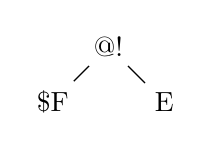
\begin{tikzpicture}
    \node(app) {@!};
    \node(f) [below left of=app]{$\textdollar$F};
    \node(E) [below right of=app]{E};
    \draw (app) -- (f);
    \draw (app) -- (E);
  \end{tikzpicture}

\item annotate supercombinator that arg. is strict

  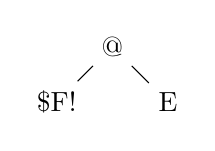
\begin{tikzpicture}
    \node(app) {@};
    \node(f) [below left of=app]{$\textdollar$F!};
    \node(E) [below right of=app]{E};
    \draw (app) -- (f);
    \draw (app) -- (E);
  \end{tikzpicture}
  
\end{itemize}

need both of the above to enable maximal parallelism

\subsection{speculative parallelism}
may waste resource

prioritize vital tasks over speculative ones

speculative tasks may cahgen to be vital when its results are discovered to be needed (some of its subgraph tasks may also change priority to vital)

speculative tasks may be stopped and discarded when result is not needed: all subtasks/sparks  need also be killed

\subsection{blocking mechanism}

mark node during unwinding of spine (when finding a function at the tip of the spine) to indicate nodes are currently being worked on

other tasks blocked when encountering marked nodes

rewinding of spine (popping of vertebrae from its stack) also removes the mark from vertebrae (after reduction overwrites its result) $\implies$ task blocked by affected nodes can proceed (and will see updated redex performed by earlier task)

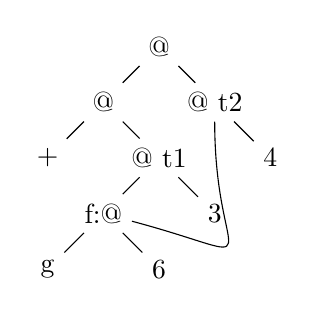
\begin{tikzpicture}
  \node(a) {@};
  \node(b) [below left of=a]{@};
  \node(plus) [below left of=b]{+};
  \node(c) [below right of=b]{@ t1};
  \node(d) [below right of=a]{@ t2};
  \node(f) [below left of=c]{f:@};
  \node(g) [below left of=f]{g};
  \node(six) [below right of=f]{6};
  \node(three) [below right of=c]{3};
  \node(four) [below right of=d]{4};
  \draw (a) -- (b);
  \draw (b) -- (plus);
  \draw (b) -- (c);
  \draw (c) -- (f);
  \draw (f) -- (g);
  \draw (f) -- (six);
  \draw (c) -- (three);
  \draw (a) -- (d);
  \draw (d) -- (four);
  \draw[-] (d) to [out=270, in=345, looseness=3] (f);
\end{tikzpicture}

if task t1 unwinds and reaches f first, then task t2 may block when unwinding to f

optimization:
\begin{itemize}
\item once a node (subgraph) is in WHNF, it will never need to be updated again $\implies$ give read-only access to $>1$ tasks concurrently (discriminate with regular application node by WHNF application node type)
\item unwinding to a WHNF application node$\implies$ node does not need to get marked (no blocking to other tasks)
\item example nodes in WHNF: supercombinator, number, cons cell
\item otherwise, nodes not in WHNF $\implies$ subgraph may contain redexes and be altered; only 1 task accesses it at any time
\end{itemize}


runtime WHNF optimization possible even if compile-time WHNF optimization is not possible

eg: (\$G E1 E2 E3)

after 1st reduction at top node, the lower 2 application nodes are in WHNF $\implies$ mark these 2 nodes as WHNF when finishing reduction (as these nodes are popped off the stack)

representation of task:
\begin{itemize}
\item store info. to restore execution of it during suspended state
  typically in a task control block:
  \begin{itemize}
  \item task stack pointer
  \item task program counter
  \item state of task's registers
  \end{itemize}
\item vs. graph representation / parellel reduction model
  \begin{itemize}
  \item a task corresponds to a subgraph that it is evaluating (state of partially completed task encoded in the graph):
  \item using a pointer to the root of the subgraph is theoretically sufficient to represent the task at any stage of its lifetime
  \item suspension of a task: stop reduction; save pointer to task's root node to the task pool
  \item resuming a task: take its pointer to root and continue reduction
  \end{itemize}
\end{itemize}

\subsection{optimization to suspending and resuming task}

uses pointer reversal to avoid unwinding spine when resuming a blocked task (avoids repeatedly unwinding spine every time a task is blocked):
\begin{itemize}
\item reverse only pointers in vertebrae (marked nodes) $\implies$ no other tasks will access a pointer reversed node
\item state of a task represented by 2 pointers (fwd and backward pointers) $\implies$ suspended task resumed: forward and backward pointers point to area of graph of interest
\item re-reversing pointers when rewinding the spine and marking vertebrae nodes as WHNF at the same time
\end{itemize}

stack based G-machine for parallel machine
\begin{itemize}
\item as a sequence of optimizations to graph reduction
\item part of state held in stack
\item at any point, info. in stack can be used to flush and update teh graph that repr. its current state
\item keep some state of the graph in stack, over some sequence of reduction steps, as optimization
\end{itemize}


when a task is blocked:
\begin{itemize}
\item return it to the task pool for future exeuction, or
\item asynchronously reawaken (put into task pool) the task once the blocked node has its mark removed (for efficiency)

  possible impl.:
  \begin{itemize}
  \item add a list of tasks to be reawakened to each application node
  \item when application node is unmarked, move reawakening taks to task pool
  \end{itemize}
\end{itemize}

\subsection{locality and distributed memory scheme}

\begin{itemize}
\item heuristics: execute tasks and allocations in some memory unit
\item parallelism vs. concurrency consideration
\item program annotation
\item heuristics to migrate tasks to memory units that are referenced  by the tasks
\item granularity of task: worthwhile to migrate large computations in a task
\end{itemize}

\vfill\null
\columnbreak

\section{FP: push/enter vs. eval/apply \cite{marlow2004}}

currying in the case of unknown functions at runtime; otherwise for known function: prep args on stack/register and call function directly

\subsection{push/enter}

callee responsibility wrt. function arity matching; function is in control: grab top args from stack (deduce number of args from a special register / frame pointer and stack pointer)

arg continuation

use of stack to hold args pending for next call to a function

no return address

each function compiled with 2 entry points:
\begin{itemize}
\item fast entry: args in register plus overflow args on stack
\item slow entry: all args on stack
\end{itemize}

argument satisfaction check (enough arguments for unknown function/call):
\begin{itemize}
\item fail: build a Partial Application (PAP) value, return to return address pointed to by a special register / frame pointer
\item success: loads args into registers and jump/fall thru. to fast entry point
\end{itemize}

periods in between production and consumption, arbitrary layout in its region of strac kdata structure; GC would not know how to deal with them; one solution is to add tag to discriminate pointer, non-pointer(include size), and return address Arg continuation

example impl. in G-machine

\subsection{eval/apply}

caller responsibility wrt.functon arity matching

call continuation pushed onto the stack to hold excess args that the function canoot take

RetRun: similar to Ret except return a function value (PAP / FUN) to call continuation $\implies$ re-activates a call continuation constructed earlier

call continuation, of form
\begin{lstlisting}
($\bullet$ $a_1$ .. $a_n$)
\end{lstlisting}
represented by stack frame with:
\begin{itemize}
\item a return address (entered when function has evaluated to a value (FUN or PAP) and returns
\item arguments $a_1$ .. $a_n$
\end{itemize}

pregeneration of a range of call continuation return addresses for 1..N arguments

multiple continuations (each with N args)  may be needed if number of args is large (>N)

no distinguishment between heap pointer and return address

return address is info pointer, where layout (locations of pointers/non-pointers) of frame is known

stack frame looks like heap object

frame is a stack allocated function closure

\vfill\null
\columnbreak

\section{Haskell Impl. Overview \cite{wiki_STG}, \cite{terei2011}}

TODO

\vfill\null
\columnbreak

\section{MLIR Notes \cite{mlir2021}, \cite{lei2022}}

\subsection{Mechanism Overview}

strucure carrying in operations via regions

conversion between different types generally correspond to transformations between different levels of abstractions

operations may be used at different abstraction levels

favours levels of abstractions and progressive lowering wwith intra dialect conversions

organization of related types and operations using dialects

tensor and memref contain ops for tiled IR structure and shape manip facilities

arith and math ops: payload ops for composing with payload carrying structured ops; work on multiple abstraction levels

vector dialect: another rdialect for structured code generation like linalg; chip register level (more H/W architecture facing and constraints)

lowering in aspects:
\begin{itemize}
\item decomposition (via tiling / vectorization)
\item abstract to concrete concepts (eg: resource assignments)

\end{itemize}

\subsection{Structured Operations}

structured operations contains compute payload (eg: attached via operations in basic block in a region)

access patterns in structured operations such as \verb|linalg.generic| op using indexing maps for inputs and output

\begin{lstlisting}
indexing_maps = [ affine_map<(d0,d1,...) -> (...)>,
                  affine_map<(d0,d1,...) -> (...)>,
                  ...]

where:
LHS of affine_map defines induction variables
RHS of affine_map contains the expression using
  induction variables
\end{lstlisting}

dimension preservation/reduction of the output via \verb|iterator_types|

\verb|memref| transforms using buffers reuse an intial buffer passed in as an input

\verb|tensor| transforms using tensors creates new value as output where initial tensor passed in does not get modified but only read

example of affine maps:

\begin{lstlisting}
[[d0,d1,d2,d3],
 [d0,d1]]

$\Updownarrow$

SmallVector<AffineMap>{
  rewriter.getMultiDimIdentityMap(4),
  AffineMap::get(4,0,{mlir::getAffineDimExpr(0,ctx),
                      mlir::getAffineDimExpr(1,ctx), ctx})}
 
\end{lstlisting}

example of compute payload attached to \verb|linalg.generic| op:

\begin{lstlisting}
ins(%1: tensor<?x?x?x?xf32>)
outs(%5: tensor<?x?xf32>){
  // arg1 <-> %1, arg2 <-> %5
  ^bb0(%arg1: f32, %arg2: f32):
    % 17 = arith.addf %arg2, %arg1 : f32
    // yield to %5
    linalg.yield %17 : f32
} -> tensor<?x?xf32>

$\Updownarrow$

[&](OpBuilder& b, Location loc, ValueRange args){
  Value input = args[0];
  Value sum = args[1];
  Value result = rewriter.create<arith::AddFOp>(
    loc, sum, input
  );
  b.create<linalg::YieldOp>(loc, result);
})
\end{lstlisting}

\subsection{Bufferization}

conversion from a tensor abstraction level to a more concrete resource level with memref dialect

goals: use less memory and copy less memory

reuse memory need to make sure data that are live are not overwritten

more complex to analyze due to presence of aliasing and dependency issues

post-bufferization: distribute to different H/W tiles

ownership based buffer deallocation pass separate from bufferization pass

\subsubsection{Destination Passing Style (DPS)}

op implement \verb|DestinationStyleOpInterface|

return result with updated value

output operands (not modified but copied) used as possible anchor for bufferization algo.

when no conflicting (eg: dependency conflicts) uses (detection via bufferization algo. / use-def chains) of result tensor in DPS corresponding to an operand, it may be aliased with that operand and perform op in-place using the buffer allocated for the corresponding tensor operand; otherwise, allocate new buffer for result

tensor ops not in DPS always bufferize to memory allocation

tensor/memref boundary helper functions:
\begin{itemize}
\item \verb|bufferization.to_memref|: returns future buffer of a tensor SSA value
\item \verb|bufferization.to_tensor|: returns a tensor SSA value for a memref buffer
\end{itemize}

\subsubsection{One Shot Bufferize}
pass with DPS and aggressive in-place bufferization

2 phases: analysis, rewrite IR (bufferize)

ops implementing \verb|BufferizableOpInterface| can be bufferized

whole function at a time analysis

\vfill\null
\columnbreak

\subsection{Vector Dialect}

convert static shaped ops to vector ops of same shape

allows further mapping to concrete hardware architectures (eg: vector instructions and registers) via more transforms such as unrolling transforms in later stages

typically used after tensor tiling

unrolling pattern may be different for different vector ops; unrollable ops implement \verb|VectorUnrollOpInterface|

high dimensional vectors: drop leading unit dimnesions before hoisting

hoisting: inspect loop carried tensors to see if we have: \verb|vector_transfer_read| at beginning and \verb|vector.transfer_write| op at end and indices are static; hoist via \verb|linalg::hoistRedundantVectorTransferOnTensor()| or \verb|linalg::hoistRedendantVectorTransfers()|

lowering: collect patterns for different ops via vector::populateVector*LoweringPatterns(); controlling lowering of specific ops to lower level operations

vectorization transformations:
\begin{itemize}
\item \verb|transfer_read, transfer_write, contract| ops
\item various modes of load/store and stride and padding supports
\end{itemize}

unroll, decomposition to lower high D vector ops into low D to match H/W architecture

low level dialects: transformation are mostly canonicalization / cleanup and not optimizations

\vfill\null
\columnbreak

\subsection{Structured Linalg}

preserve structure of computation for as long as possible to enable ease of certain types of transformations

patterned compute / data rearrangement operations

implicit perfect loop nest: less analysis required, easier to transform 

explicit loop iterator type

input/output opereand has associated indexing map which specify access of operand's elements
loop iteration space derived from op's operands

use of region to hold computation

operations not using perfect loop nests require custom handling

with tensor: op result has associated output operand providing initial value

with buffer: no result; output operand is mutable buffer

sample useful constructs and mechanisms provided
\begin{itemize}
\item tiling: division of data into smaller ones, allowing utilization of multiple compute units; interface provides tiling strategy of the op
\item fusion
\item elementwise extension to high rank arrays
\item reduction on vectors via native vector support (\verb|vector.reduction<reduction_type>|, transform into loop (\verb|scf.for|)
\item contraction of 2 input arrays via use of \verb|indexing_maps, iterator_types|
\end{itemize}

some properties of \verb|linalg.generic|:
\begin{itemize}
\item explicitly contains a region (block args corresponds to individual elements of operands of \verb|ins| and \verb|outs|) for computation (arbitrary operations)
\item destination passing style
\item work on buffers (\verb|tensor|) or memory (\verb|memref|)
\item out operands read and writable
\item output operands used only as initialization values for tensor and memory; result is a new tensor
\item memory allocation of result may be elided (becomes an in-place operation) if compiler can prove no other things mutates the output operand
\item if output operand is a tensor, result is always a new tensor (allocated)
\end{itemize}

serveral sample useful operations provided by the transform dialect:
\begin{itemize}
\item \verb|transform.named_sequence| for defining transformation and allow chaining of operations
\end{itemize}

\subsubsection{Definitions}

payload IR: target IR to undergo transformation

transform IR: IR that defines the transformation

materialization: description for how a list of values should be converted to a list of values with specific types (may produce IR). types of materialization:
\begin{itemize}
\item source materialization: value replaced with a value of different type, but expects source type by some users, so the materialization converts the replacement value back to the source type
\item target materialization: converts a value to type that is expected by a conversion pattern specified by type converter
\end{itemize}

types of argument/handle to transform dialect operation:
\begin{itemize}
\item operation (value operation)
\item value (value handle)
\item attribute (value parameter)
\end{itemize}

\subsubsection{Affine Map}
used for defining use of induction variables by input and output elements via \verb|indexing_maps|

\subsubsection{Iterator Types}
\verb|iterator_types|: one of parallel/reduction

\subsubsection{Tiling}

leads to vectorization or materizalization of loop nest (eg: \verb|scf.for|) and inlining of compute region

embedding of structures in op semantics (multiple constructs inside together to make it work)

general strategy:
\begin{enumerate}
\item extract subslice from original source data (\verb|tensor.extract_slice|)
\item do computation on subslice
\item insert computed result back into associated subslice of result data (\verb|tensor.parallel_insert_slice|)
\end{enumerate}

\subsubsection{Fusion}
use inverse of \verb|indexing_mapping| to go from tiled consumer op back to producer op to also pull in producer op into the materialization loop associated with tiling

adapt and recompute as necessary by fusing preceding operations into loops

recomputation/rematerialization vs. storage tradeoff

\subsubsection{Vectorization}
mechanically convert to vector ops (which are later lowered to lower dimensional ones) and preserve shape

\subsubsection{Distribution}

assign tiles to compute units

provide info when tiling / fusing

materialized loop nest: modify loop ranges with info

\subsubsection{IR Modifications}

IR changes tracked during transform via provided rewriter:
\begin{itemize}
\item payload op erase $\implies$ auto-removed from all handles associated with it
\item payload op replaced $\implies$ dialect find replacement op and updates all associated handles
\end{itemize}

transform operations may consume operand handle if payload ops erased or recreated: any alias to consumed handle are invalidated

\subsection{Dialect Extension}
inject new operations into an existing dialect via registration

\verb|TransformDialectExtension<MyExtension>| for Transform dialect extension; within \verb|init()| function:

specify dependent dialect that have attributes or types used by transofmr operations via \verb|declareDependentDialect<...>()|

specify attributes, operations, and types generated by the transformation via  \verb|declareGeneratedDialect<...>()|

register new operations via \verb|registerTransformOps<...>()|

new operations definable with ODS in the same way as regular ops in a dialect

use of Tablegen and CMake to generate header and impl of operations to be included in declaration and definition of transform operations via \verb|#define GET_OP_CLASSES / #define GET_OP_LIST| before including \verb|*.cpp.inc| file

enable extension from project main driver by calling registration hook

\subsection{Notable Interfaces}

\verb|TransformOpInterface|

\verb|DeclareOpInterfaceMethods|

\subsection{Type Constraints and ApplyEach Trait}
use Transform dialect types to specific preconditions of type of each payload operation (eg: narrowing from \verb|TransformHandleTypeInterface| to \verb|Transform_ConcreteOp<''func.call''>|

helper trait \verb|TransformEachOpTrait| provides impl. of ``apply'' trait that:
\begin{itemize}
\item verifies
\item iterates over payloads
\item result concatenation
\end{itemize}

\subsection{Consuming Operand Handle of Payload}

rewrite and produce a new operation and indicate side effects via \verb|modifiesPayload(effects)| within \verb|getEffects()| of \verb|MemoryEffectsOpInterface|

\subsection{Matching Payload with Transform Operations}

goal: caller does not need to identify payload operations when invoking a transform; let matcher identify payload operations that need to be transformed

creation of custom types to constraint payload operation types vis ODS

enable custom types and attributes in dialect extension via registeration hooks, eg:
\begin{lstlisting}
registerTypes<
  #define GET_TYPEDEF_LIST
  #include *.cpp.inc
>()
\end{lstlisting}

not expected to modify payload IR

expeced to fail if match operation's operands are not associated with payload IR object with desired properties )eg: op name, argument kinds)

discover relevant operations in payload IR via match ops instead of explicit actions by caller

use of \verb|transform.match.operation_name|

chaining of match operations in a matcher sequence (eg: matching multiple ops connected locally) to enable a bigger contextual match

match operation is similar to other transform operations, plus additional implementation of \verb|MatchOpInterface| (only used as verification contract that op will not attempt to transform the payload)

custom match operation definable in ODS (eg: make it implement \verb|TransformOpInterface, MemoryEffectsOpInterface|); implement \verb|apply()| method for \verb|TransformOpInterface| and \verb|getEffects()| method for \verb|MemoryEffectsOpInterface|; test nested matchers (accessed thru a region's block) for matching condition

\subsubsection{Matching for Inferred Features}

matching for properties derivable from operations of interest and checking for constraints (eg: such as dimension access from access maps of inputs are consistent)

\subsection{Rewrite Alternatives}
\begin{itemize}
\item PDL
\item C++ rewriting API
\end{itemize}

\vfill\null
\columnbreak

\bibliographystyle{plain}
\bibliography{notebook}
    
\end{multicols*}

\end {document}
